% ........................................................................... %

\documentclass[a4paper,12pt]{memoir}

% ........................................................................... %

\usepackage[
	a4paper,
	pdftitle = {Model-based~analysis~of~time-aware~web~services~interactions},
	pdfauthor = {Julien~Ponge},
	pdfsubject = {PhD~Thesis},
	pdfkeywords = {
		web~
		service~
		soa~
		timed~
		protocol~
		automata~
		analysis~
		compatibility~
		replaceabilty~
		servicemosaic~
	},
	pdfview = {FitH},
	pdfstartview = {FitH},
	pdfborder = {0 0 0},
	colorlinks = true,
	linkcolor = black,
	citecolor = blue,
	filecolor = blue,
	urlcolor = blue
]{hyperref}
\usepackage{memhfixc}

\usepackage[T1]{fontenc}
\usepackage{lmodern}
\usepackage[latin1]{inputenc}

\usepackage{url}
\urlstyle{sf}

\usepackage{graphicx}

\usepackage{amsmath}
\usepackage{amsfonts}
\usepackage{amssymb}
\usepackage{amsthm}

\usepackage{multirow}
\usepackage{moreverb}

\usepackage[sort&compress,square,colon,numbers]{natbib}

% ........................................................................... %

\renewcommand{\cite}[1]{(\citet{#1})}

\newtheorem{definition}{Definition}
\newtheorem{theorem}{Theorem}
\newtheorem{corollary}{Corollary}
\newtheorem{lemma}{Lemma}
\newtheorem{property}{Property}
\newtheorem{procedure}{Procedure}

% ........................................................................... %

\newcommand{\R}{\mathbb{R}}
\newcommand{\Q}{\mathbb{Q}}
\newcommand{\N}{\mathbb{N}}
\newcommand{\Rpos}{\R_{\geq 0}}
\newcommand{\Qpos}{\Q_{\geq 0}}
\newcommand{\T}{\mathbb{T}}
\newcommand{\val}{\mathcal{V}}

\newcommand{\tm}{\texttrademark~}

\newcommand{\CInvoke}{ \mbox{C-Invoke} }
\newcommand{\MInvoke}{ \mbox{M-Invoke} }

\DeclareMathOperator{\Polarity}{Polarity}
\newcommand{\polarity}[2]{\Polarity(#1, #2)}

\newcommand{\compop}{ \parallel^{\mathtt{TC}} }
\newcommand{\intersop}{ \parallel^{\mathtt{TI}} }
\newcommand{\diffop}{ \parallel^{\mathtt{TD}} }
\newcommand{\projop}[3]{ \left[ #1 \compop #2 \right]_{#3} }

\DeclareMathOperator{\map}{map}
\DeclareMathOperator{\inhib}{inhib}
\DeclareMathOperator{\permits}{permits}

% ........................................................................... %

% UNSW (strict) requirements
%
% \settrimmedsize{242mm}{150mm}{*}
% \settrims{30mm}{20mm}
% \setlrmarginsandblock{1mm}{1mm}{*}
% \setlength{\uppermargin}{\headheight} \addtolength{\uppermargin}{\headsep}
% \setlength{\lowermargin}{\uppermargin}
% \setlength{\textheight}{\paperheight} \addtolength{\textheight}{-2\uppermargin}
% \checkandfixthelayout

\OnehalfSpacing

\maxtocdepth{subsection}
\maxsecnumdepth{subsection}

\chapterstyle{demo}
\pagestyle{ruled}

% ........................................................................... %

\begin{document}

% ........................................................................... %

\frontmatter

%% ........................................................................... %

\begin{titlingpage}

\noindent \footnotesize{N� d'ordre : D.U. 1840}

\noindent \footnotesize{EDSPIC : 402}

\vfill

\begin{center}
	\textbf{Universit� Blaise Pascal -- Clermont-Ferrand II}
	
	\'Ecole Doctorale des Sciences pour l'Ing�nieur de Clermont-Ferrand \\[0.75em]
	
	\textbf{The University of New South Wales, Sydney, Australia}
	
	School of Computer Science and Engineering
\end{center}

\vfill

\begin{center}
	\Large{\textbf{Th�se}}
	
	\footnotesize{pr�sent�e par}
	
	\large{\textbf{Julien PONGE}}
	
	\footnotesize{pour obtenir le grade de}
	
	\large{\textbf{Docteur d'Universit�}}
	
	\large{\textbf{Sp�cialit� :} Informatique}
\end{center}

\vfill

\begin{center}
	\Large{\textbf{\textsf{Model Based Analysis of Time-aware Web Services Interactions}}}
\end{center}

\vfill

\begin{center}
	
	\begin{tabular}{l}
		Th�se dirig�e par Farouk TOUMANI / Boualem BENATALLAH \\		
		Soutenue publiquement le 1\textsuperscript{er} Juillet 2008 devant le jury suivant : \\
	\end{tabular}
	
	\vspace{1em}
	
	\begin{center}
	\begin{tabular}{r l}
		Prof. Marie-Christine FAUVET & Pr�sidente \\
		Prof. Schahram DUSTDAR & Rapporteur \\
		Prof. Claude GODART  & Rapporteur \\
		Prof. Marlon DUMAS & Examinateur \\
		Prof. Michel SCHNEIDER & Examinateur \\
		Prof. Farouk TOUMANI & Directeur de Th�se  (UBP) \\
	 	Prof. Boualem BENATALLAH & Directeur de Th�se (UNSW) \\
	\end{tabular}
	\end{center}
	
\end{center}

\end{titlingpage}

% ........................................................................... %

\cleardoublepage
% ........................................................................... %

\paragraph{Abstract.}

Web services are increasingly gaining acceptance as a framework for facilitating
application-to-application interactions within and across enterprises. It is commonly accepted that a service description should include not only the interface, but also the \emph{business protocol} supported by the service. The present work focuses on the formalization of the important category of protocols that include time-related constraints (called \emph{timed protocols}), and the impact of time on compatibility and replaceability analysis.

We formalized the following timing constraints: \CInvoke constraints define time windows of availability while \MInvoke constraints define expirations deadlines. We extended techniques for compatibility and replaceability analysis between timed protocols by using a semantic-preserving mapping between timed protocols and timed automata, leading to the novel class of \emph{protocol timed automata} (PTA). Specifically, PTA exhibit silent transitions that cannot be removed in general, yet they are closed under complementation, making every type of compatibility or replaceability analysis decidable. Finally, we implemented our approach in the context of a larger project called ServiceMosaic, a model-driven framework for web service life-cycle management.

\paragraph{Keywords.}
Web services; timed business protocols; compatiblity and replaceability analysis; choreography; orchestration; business process; service-oriented architectures; timed automata.

% ........................................................................... %

\cleardoublepage
% ........................................................................... %


\paragraph{R�sum�.}


Les services web gagnent de l'importance en tant que cadre facilitant l'int�gration d'applications au sein et en dehors des fronti�res des entreprises. Il est accept� que la description d'un service ne devrait pas seulement inclure l'interface, mais aussi le protocole m�tier support� par le service. Dans le cadre de ce travail, nous avons formalis� la cat�gorie des protocoles incluant des contraintes de temps (appel�s \emph{protocoles temporis�s}) et �tudi� l'impact du temps sur l'analyse de compatibilit� et de rempla�abilit�.


Nous avons formalis� les contraintes suivantes : les contraintes \CInvoke d�finissent des fen�tres de disponibilit�s tandis que les contraintes \MInvoke d�finissent des d�lais d'expiration. Nous avons �tendu les techniques pour l'analyse de compatibilit� et de rempla�abilit� entre protocoles temporis�s � l'aide d'un mapping pr�servant la s�mantique entre les protocoles temporis�s et les automates temporis�s, ce qui a d�fini la classe des \emph{automates temporis�s de protocoles} (PTA). Les PTA poss�dent des transitions silencieuses qui ne peuvent pas �tre supprim�es en g�n�ral, et pourtant ils sont ferm�s par calcul du compl�ment, ce qui rend d�cidable les diff�rents types d'analyse de compatibilit� et de rempla�abilit�. Enfin, nous avons mis en oeuvre notre approche dans le cadre du projet ServiceMosaic, une plate-forme pour la gestion du cycle de vie des services web.


\paragraph{Mots-cl�s.}

Services web; protocoles m�tiers; compatibilit�; rempla�abilit�; analyse; chor�graphie; orchestration; processus m�tier; architectures orient�es-services; automates temporis�s.


% ........................................................................... %

\cleardoublepage
% ........................................................................... %

~

\vfill

\noindent
This work was conducted at the LIMOS Laboratory (Laboratoire d'Informatique, de Mod�lisation et d'Optimisation des Syst�mes), Universit� Blaise Pascal, Clermont-Ferrand, France:\\

\noindent
\textsf{%
LIMOS \\
Complexe scientifique des C�zeaux \\
63177 Aubi�re cedex \\
France
}

\vspace{4em}

\noindent
This work was also conducted under \emph{cotutelle agreements} at the School of Computer Science and Engineering, The University of New South Wales, Sydney, Australia:\\

\noindent
\textsf{%
School of Computer Science and Engineering \\
UNSW Kensington Campus \\
The University of New South Wales \\
Sydney \\
NSW 2052 \\
Australia
}

\vfill

% ........................................................................... %

\cleardoublepage
% ........................................................................... %

\section*{Acknowledgments}

The story behind this PhD thesis started in 2004 while a Master by Research student at the Universit� Blaise Pascal in Clermont-Ferrand. As I was looking for an internship topic, Michel Schneider pointed me to Farouk Toumani, who would eventually become my PhD adviser. Thank you Michel for that, as Farouk proved to be a very good adviser. During those 4 years working on this topic, he always provided good guidance and support. It has been a great pleasure to work with him, both from a professional and a personal point of view. In turn, Farouk pointed me to Boualem Benatallah, who would become my PhD adviser at the University of New South Wales as I did my PhD \emph{under cotutelle agreements} between the two universities. I enjoyed working with Boualem very much, and his advices turned out to complement nicely those from Farouk.

I would like to thank the people with whom I shared the office room: Yoan Renaud that I first met when I entered the university, Alain G�ly and Olivier Coupelon. We have had some great time together, and I am sure that there is still a lot more to come. There is a special mention for a group of 4 students of mine who later became my friends: Pierre Colomb, Olivier Montagner, Olivier Passalacqua and Fr�d�ric Desforges. Of course I have enjoyed working with many other colleagues and friends in Clermont-Ferrand: Ramy Ragab, Marie Agier, Olivier Raynaud, Fr�d�ric Flouvat, H�l�ne Jaudoin, St�phanie Chollet, Kevin Hivernat, Yannick Loiseau, Raoul M�dina, B�atrice Bourdieu and Fran�oise Toledo.

I would like to thank my coauthor Fabio Casati for the good times we have had working together, and for his never ending positive attitude. I met a lot of great people during my visits at UNSW. Warm thanks go to my friend Hamid Motahari and his wife Razieh for their kindness and for making my discovery of life in Australia so much easier. Among the people I met there, I would like to thank Halvard Skogsrud and Woralak Kongdenfha. Special thanks go to Mohand-Said Hacid that I first met while in Sydney. We spent some great time at UNSW, and he taught me a lot regarding running training!

Many thanks go to my reviewers and examiners as part of the French side of my PhD defense: Marie-Christine Fauvet, Schahram Dustdar, Claude Godart, Marlon Dumas and Michel Schneider. It has been a great honor to have you all as part of the examination committee!

My warmest thanks naturally go to my family, my parents Evelyne and Jean for having always stood behind me through the good and the bad times. I would probably not have gone so far in my studies without their encouragements and the education that they gave me. My final -- and biggest -- thanks go to Marie-Anne for her love and steady support during all of these years. Doing this PhD has required some sacrifices and I am deeply grateful to her not only because she accepted them, but because she fully and wholeheartedly endorsed them.

% ........................................................................... %

% ........................................................................... %
% ........................................................................... %

\begin{titlingpage}

\begin{center}
	\LARGE{\textbf{\textsf{Model Based Analysis of Time-aware Web Services Interactions}}}
	
	\normalsize
	
	\vfill
	
	
\includegraphics[width=3cm]{content/UNSW_crest}
	
	The University of New South Wales
	
	Sydney, Australia
	
	\vfill
	
	Universit� Blaise Pascal -- Clermont-Ferrand 2
	
	France
	
	\vfill
	
	A dissertation submitted in fulfillment
	
	of the requirements for the degree of 
	
	\Large{Doctor of Philosophy}
	
	\normalsize
	
	in
	
	\Large{Computer Science and Engineering}
	
	\normalsize
		
	\Large{\textsl{(under cotutelle agreements)}}
	
	\vfill
	
	\normalsize
	
	\Large{Julien Ponge}
	
	\vfill
	
	\normalsize
	
	\begin{tabular}{rl}
	Supervisors: & Prof. Boualem Benatallah \\
	             & Prof. Farouk Toumani \\
	\end{tabular}
	
	\vfill
	
	Final version, January 2009
	
\end{center}

\end{titlingpage}

% ........................................................................... %

\thispagestyle{empty}

\section*{Originality Statement}

\textsl{``I hereby declare that this submission is my own work and to the best of my
knowledge it contains no materials previously published or written by
another person, or substantial proportions of material which have been
accepted for the award of any other degree or diploma at UNSW or any other
educational institution, except where due acknowledgment is made in the
thesis. Any contribution made to the research by others, with whom I have
worked at UNSW or elsewhere, is explicitly acknowledged in the thesis. I
also declare that the intellectual content of this thesis is the product of my
own work, except to the extent that assistance from others in the project's
design and conception or in style, presentation and linguistic expression is
acknowledged.''} \\[3em]

\noindent Julien Ponge \\
\noindent January 2009

\clearpage

% ........................................................................... %

\thispagestyle{empty}

\section*{Copyright Statement}

\textsl{``I hereby grant the University of New South Wales or its agents the right to archive and to make available my thesis or dissertation in whole or part in the University libraries in all forms of media, now or here after known, subject to the provisions of the Copyright Act 1968. I retain all proprietary rights, such as patent rights. I also retain the right to use in future works (such as articles or books) all or part of this thesis or dissertation.
I also authorise University Microfilms to use the 350 word abstract of my thesis in Dissertation Abstract International (this is applicable to doctoral theses only).
I have either used no substantial portions of copyright material in my thesis or I have obtained permission to use copyright material; where permission has not been granted I have applied/will apply for a partial restriction of the digital copy of my thesis or dissertation.''} \\[3em]

\noindent Signed ...........................\\
\noindent January 2009

\clearpage

% ........................................................................... %

\thispagestyle{empty}

\section*{Authenticity Statement}

\textsl{``I certify that the Library deposit digital copy is a direct equivalent of the final officially approved version of my thesis. No emendation of content has occurred and if there are any minor variations in formatting, they are the result of the conversion to digital format.''}\\[3em]

\noindent Signed ...........................\\
\noindent January 2009

\clearpage

% ........................................................................... %

% ........................................................................... %

~

\vfill

\noindent
This work was conducted at the LIMOS Laboratory (Laboratoire d'Informatique, de Mod�lisation et d'Optimisation des Syst�mes), Universit� Blaise Pascal, Clermont-Ferrand, France:\\

\noindent
\textsf{%
LIMOS \\
Complexe scientifique des C�zeaux \\
63177 Aubi�re cedex \\
France
}

\vspace{4em}

\noindent
This work was also conducted under \emph{cotutelle agreements} at the School of Computer Science and Engineering, The University of New South Wales, Sydney, Australia:\\

\noindent
\textsf{%
School of Computer Science and Engineering \\
UNSW Kensington Campus \\
The University of New South Wales \\
Sydney \\
NSW 2052 \\
Australia
}

\vfill

% ........................................................................... %

\cleardoublepage
% ........................................................................... %

\paragraph{Abstract.}

Web services are increasingly gaining acceptance as a framework for facilitating
application-to-application interactions within and across enterprises. It is commonly accepted that a service description should include not only the interface, but also the \emph{business protocol} supported by the service. The present work focuses on the formalization of the important category of protocols that include time-related constraints (called \emph{timed protocols}), and the impact of time on compatibility and replaceability analysis.

We formalized the following timing constraints: \CInvoke constraints define time windows of availability while \MInvoke constraints define expirations deadlines. We extended techniques for compatibility and replaceability analysis between timed protocols by using a semantic-preserving mapping between timed protocols and timed automata, leading to the novel class of \emph{protocol timed automata} (PTA). Specifically, PTA exhibit silent transitions that cannot be removed in general, yet they are closed under complementation, making every type of compatibility or replaceability analysis decidable. Finally, we implemented our approach in the context of a larger project called ServiceMosaic, a model-driven framework for web service life-cycle management.

\paragraph{Keywords.}
Web services; timed business protocols; compatiblity and replaceability analysis; choreography; orchestration; business process; service-oriented architectures; timed automata.

% ........................................................................... %

% ........................................................................... %

\cleardoublepage

\section*{Publications}

Some parts and preliminary results presented in this dissertation have been published.

\subsection*{International refereed conferences}
\begin{itemize}

	\item Julien Ponge, Farouk Toumani, Boualem Benatallah and Fabio Casati. \textbf{Fine-grained Compatibility and Replaceability Analysis of Timed Web Service Protocols}. \emph{In the 26th International Conference on Conceptual Modeling (ER).} Auckland, New Zealand. November 2007.
	
	\item Boualem Benatallah, Fabio Casati, Julien Ponge and Farouk Toumani. \textbf{On Temporal Abstractions of Web Services Protocols}. \emph{Proceedings of CAiSE Forum 2005.} Porto, Portugal. June 2005.

\end{itemize}

\subsection*{National refereed conferences}
\begin{itemize}

	\item Boualem Benatallah, Fabio Casati, Julien Ponge, Farouk Toumani. \textbf{Compatibility and replaceability analysis for timed web service protocols}. \emph{In BDA 2005}. Saint-Malo, France. October 2005.

\end{itemize}

\subsection*{Refereed journals}
\begin{itemize}
    
    \item Julien Ponge, Boualem Benatallah, Fabio Casati and Farouk Toumani. \textbf{Analysis and Applications of Timed Service Protocols}. To appear in ACM Transactions on Software Engineering and Methodology (TOSEM).

	\item Boualem Benatallah, Fabio Casati, Farouk Toumani, Julien Ponge and Hamid Reza Motahari Nezhad. \textbf{Service Mosaic: A Model-Driven Framework for Web Services Life-Cycle Management}. \emph{IEEE Internet Computing, vol. 10, no. 4, pp. 55-63}. July/August 2006.

\end{itemize}

\subsection*{Refereed workshops and demonstrations}
\begin{itemize}

	\item Hamid Motahari, Regis Saint-Paul, Boualem Benatallah, Fabio Casati, Julien Ponge and Farouk Toumani. \textbf{ServiceMosaic: Interactive Analysis and Manipulations of Service Conversations}. \emph{In International Conference on Data Engineering (ICDE'07).} Istanbul, Turkey. April 2007.
	
	\item Julien Ponge, \textbf{A New Model For Web Services Timed Business Protocols}. \emph{Atelier ``Conception des systemes d'information et services Web''- Conf\'erence INFORSID. Hammamet}. Tunisia, May 2006.
	
	\item Julien Ponge, \textbf{Modeling and Analysing Web Services Protocols}. \emph{In IBM PhD Student Symposium at ICSOC 2005}. Amsterdam, The Netherlands, December 2005.

\end{itemize}

% ........................................................................... %

\cleardoublepage
% ........................................................................... %

\section*{Acknowledgments}

The story behind this PhD thesis started in 2004 while a Master by Research student at the Universit� Blaise Pascal in Clermont-Ferrand. As I was looking for an internship topic, Michel Schneider pointed me to Farouk Toumani, who would eventually become my PhD adviser. Thank you Michel for that, as Farouk proved to be a very good adviser. During those 4 years working on this topic, he always provided good guidance and support. It has been a great pleasure to work with him, both from a professional and a personal point of view. In turn, Farouk pointed me to Boualem Benatallah, who would become my PhD adviser at the University of New South Wales as I did my PhD \emph{under cotutelle agreements} between the two universities. I enjoyed working with Boualem very much, and his advices turned out to complement nicely those from Farouk.

I would like to thank the people with whom I shared the office room: Yoan Renaud that I first met when I entered the university, Alain G�ly and Olivier Coupelon. We have had some great time together, and I am sure that there is still a lot more to come. There is a special mention for a group of 4 students of mine who later became my friends: Pierre Colomb, Olivier Montagner, Olivier Passalacqua and Fr�d�ric Desforges. Of course I have enjoyed working with many other colleagues and friends in Clermont-Ferrand: Ramy Ragab, Marie Agier, Olivier Raynaud, Fr�d�ric Flouvat, H�l�ne Jaudoin, St�phanie Chollet, Kevin Hivernat, Yannick Loiseau, Raoul M�dina, B�atrice Bourdieu and Fran�oise Toledo.

I would like to thank my coauthor Fabio Casati for the good times we have had working together, and for his never ending positive attitude. I met a lot of great people during my visits at UNSW. Warm thanks go to my friend Hamid Motahari and his wife Razieh for their kindness and for making my discovery of life in Australia so much easier. Among the people I met there, I would like to thank Halvard Skogsrud and Woralak Kongdenfha. Special thanks go to Mohand-Said Hacid that I first met while in Sydney. We spent some great time at UNSW, and he taught me a lot regarding running training!

Many thanks go to my reviewers and examiners as part of the French side of my PhD defense: Marie-Christine Fauvet, Schahram Dustdar, Claude Godart, Marlon Dumas and Michel Schneider. It has been a great honor to have you all as part of the examination committee!

My warmest thanks naturally go to my family, my parents Evelyne and Jean for having always stood behind me through the good and the bad times. I would probably not have gone so far in my studies without their encouragements and the education that they gave me. My final -- and biggest -- thanks go to Marie-Anne for her love and steady support during all of these years. Doing this PhD has required some sacrifices and I am deeply grateful to her not only because she accepted them, but because she fully and wholeheartedly endorsed them.

% ........................................................................... %

% ........................................................................... %

\cleardoublepage

\tableofcontents
\clearpage
\listoffigures
\clearpage
\listoftables

\cleardoublepage

% ........................................................................... %

\mainmatter

\thispagestyle{plain}
\epigraph{``If you find that you're spending almost all your time on theory, start turning some attention to practical things; it will improve your theories. If you find that you're spending almost all your time on practice, start turning some attention to theoretical things; it will improve your practice.''}{Donald Knuth}

% ........................................................................... %

\part{Introduction and background}

% ........................................................................... %


\chapter{Introduction}
\label{chap:introduction}
% ........................................................................... %

The introduction of this thesis first presents the context in the field of web services and application integration. We then look at the research issues behind this work, the contributions and finally give an outline of the document.

% ........................................................................... %

\section{Context}

% ........................................................................... %

Web services are increasingly gaining acceptance as a framework for facilitating
application-to-application interactions within and across enterprises \cite{Alonso04}. Application interoperability
has been and still is a difficult issue due to difficulties created by heterogeneous and autonomous
systems. Web services provide abstractions and technologies for exposing enterprise applications as
services and make them programmatically accessible through standardized interfaces. Indeed, the main
benefit they bring to application integration is that of standardization, in terms of description
languages, coordination, and interaction protocols \cite{Alonso04,ws_cacm_special_issue,PTDL07,PH07}.
Standardization at interface definition language (WSDL) and transport protocol (SOAP) has enabled
basic interoperability at the messaging layer. Indeed, developers are using SOAP and WSDL to
integrate enterprise applications \cite{WS-standards}. This is by itself a huge improvement over previous application integration middlewares (e.g., RPC and messaging systems) as no costly adapters have to be developed so that the systems can interoperate (e.g., network protocol entry points and data representation converters).\\

While much progress has been made toward providing basic interoperability, there is still a lot to
be done to simplify service development and interaction. In particular, an important aspect of Web
services that affects interoperability is that services are loosely-coupled, that is, they are not
developed only to interact with specific clients but are meant to serve the needs of many different (and potentially unknown) 
clients, possibly developed by different teams or even different companies. Hence, developers of
client applications need to be aware of all functional and non-functional aspects of a service to be
able to understand if they can interoperate with a service and how to develop clients that can
interact correctly with the service. 
As such, service descriptions are specifications of the syntactic or semantic properties of a service that are made available to potential clients, for example with the purpose of:
\begin{enumerate}
  \item assisting developers in creating clients that can correctly use and interact with a service, and 
  \item enabling the selection, either at design time or at runtime, of services that match the clients needs.
\end{enumerate}

Hence, service descriptions need to be richer than ``just''
descriptions of interfaces as in conventional middleware (e.g, Corba IDL). Specifically, it is commonly accepted that
a service description should include not only the interface, but also the \emph{business protocol}
supported by the service, i.e., the specification of possible message exchange sequences
(conversations) that are supported by the service \cite{BBFC04}.
Tools supporting service development today are mainly concerned with interoperability at the lower
levels of the service stack (e.g. mappings from WSDL to Java and vice versa, or making two SOAP-based
systems talk to each other). There is little support for protocol modeling and management.\\

Protocols can be specified using BPEL (\emph{Business Process Execution Language} \cite{WSBPEL2}) or any of the many other formalisms developed for this purpose (e.g., \cite{BBFC04,FTBB,berardithesis}).
%
Providing service descriptions is not in itself sufficient to facilitate development and binding. In addition to descriptions, we need formal methods and software tools for automatically analyzing service descriptions to:
(i) identify if interaction between a client and a service is possible, and if it is,
(ii) identify which conversations can be carried out between two services, to help developers to check if these include all and only the desired ones, and if it is not,
(iii) understand mismatches between protocols and, if possible, create adapters to allow interactions to occur. \\

The need for formal methods and software tools for such type of analysis is widely recognized, and many approaches have been developed to this end. In \cite{BBFC04,BBFC04b,FTBB}, an approach, a model for business protocols and a framework for protocol-based analysis had been presented. The availability of such analysis concepts and tools is quite powerful in that it allows us to assess compatibility in both top-down and bottom-up development approaches. 
%
The \emph{ServiceMosaic project} \cite{BCTPM06-SM} aims at developing a model-driven framework for web service life-cycle management. Business protocol management is a key concern in the ServiceMosaic tools set. In addition to protocol design and analysis tools, it also includes facilities for adapting services at the protocol level and for discovering protocol models from service execution logs. As such, the work that we present here is being developed as part of the ServiceMosaic effort.

% ........................................................................... %

\section{Research issues}

% ........................................................................... %

The present work focuses on the important category of protocols that include time-related constraints (called \emph{timed protocols} in the following).
Time is a crucial abstraction that has been studied in several works in research fields such as workflow systems \cite{LTIM06,DMMZ06,BWJ02} and even web services \cite{berardi03finite,KazhamiakinPP06,DCPVC06}. There are countless examples of  behaviors that involve timing issues in any kind of protocol~\cite{BBFC04}, from business protocol for web services (e.g., see the \emph{RosettaNet PIPs}), to interactions between traditional web-based services and users (see E-Commerce web sites such as \emph{Travelocity} or \emph{Amazon}), to lower level protocols such as TCP. Time-related behaviors range from session timeouts to ``logical'' deadlines with different kinds of behaviors (e.g., seats reserved on a flight needs to be paid within $n$ hours otherwise they are released). However, most approaches mainly consider time for performing traditional model checking verifications such as liveness (a condition can be satisfied), safety (a condition can never be satisfied) and testing the absence of deadlocks \cite{KazhamiakinPP06,DCPVC06,berardi03finite}.\\

The work that we present here formalizes the timing constraints of the business protocol model and extends the analysis approach introduced in \cite{BBFC04,BBFC04b,FTBB}. The introduction of time aspects adds significant complexity to the problem compared to the case of ``simple'' business protocols from \cite{FTBB}.
Many formal models enabling explicit representation of time exist (e.g., \emph{timed automata}, \emph{timed petri-nets}), all showing extreme difficulties to handle algorithmic analysis of timed models.
For example, \emph{timed automata}, which are today considered as a standard modeling formalism to deal with timing constraints, suffer from undecidability of many problems such as language inclusion and complementation that are fundamental to system analysis and verification tasks \cite{RADLD94}.
Such problems have been shown to be sensitive to several criteria (e.g., density of the time axis, type of constraints, presence of silent transitions, etc) \cite{RAPM04}. \\

In our case, supporting compatibility and replaceability analysis requires tackling a number of challenges and producing several contributions, which we outline hereafter.

% ........................................................................... %

\section{Contributions}

% ........................................................................... %

Given the importance of considering time-related properties, we present a set of concepts and techniques, supported by a tool, for performing compatibility and replaceability analysis between timed protocols. The contributions are the following.

\paragraph{Timed protocols model.}
The first step consists in defining a protocol model, called \emph{timed business protocol} that enhances the business protocol model presented in \cite{BBFC04,BBFC04b,FTBB} by introducing time-related constraints.
We identified two timing constraint primitives that we added to the model for which we give both a syntax and semantics.
\begin{enumerate}

	\item \CInvoke constraints define time windows during which an action can take place (e.g., receiving a purchase order acknowledgment), and
	
	\item \MInvoke constraints define triggers for implicit actions to take place (e.g., a timeout).

\end{enumerate}
Timed business protocols provide a precise understanding of the external behavior of a service, as one knows exactly which conversations are valid with respect to both the messages ordering and the timing at which those messages are exchanged. Syntax and semantics are required for timed protocols. As timed automata \cite{RADLD94} form a widely studied model for capturing timing requirements of systems, a link between timed protocols and timed automata allowed to re-use and derive properties. We will see that the task was not straightforward, especially as \MInvoke constraints are not easy to represent equivalently in timed automata.

\paragraph{Timed protocols analysis.}
The next step consists in defining analysis concepts for identifying compatibility and replaceability between timed protocols. To do that, we extended the work of \cite{FTBB} by introducing several flexible classes for both compatibility and replaceability, and by characterizing them using a set of protocol manipulation and comparison operators. By flexible, we mean that those classes cater for more than ``black or white'' compatibility or replaceability cases like it has traditionally been done for hardware and software components, as the versatile, fast-changing nature of web services requires flexibility for such an approach to be useful.

In our timed protocol operators investigations, we chose to reuse and extend work from timed automata, and from there, we have obtained their decidability. To do that, we defined a semantic-preserving mapping between timed protocols and timed automata, leading to a novel class of timed automata that we called \emph{protocol timed automata}. The task is however not trivial, as:
\begin{itemize}
	
	\item protocol timed automata exhibit $\varepsilon$-labeled switches with clock resets that make them strictly more expressive than timed automata \cite{BBVD+99}, keeping the traditional problems of language inclusion and complementation undecidable \cite{RADLD94}, and
	
	\item \MInvoke constraints semantics are hard to implement in timed automata as we will see in chapter~\ref{chap:timed-protocols}.
	
\end{itemize}
The study of protocol timed automata allowed for two important theoretical results:
\begin{enumerate}
  
  \item the class of protocol timed automata is closed under both intersection and complementation, making it the first such one among the existing classes of timed automata having $\varepsilon$-labeled switches with resets, and
  
  \item protocol operators remain decidable in the case of timed protocols as we derive techniques from timed automata. Had the class of protocol timed automata not been closed under complementation, those results would not have hold true.
  
\end{enumerate}

\paragraph{ServiceMosaic prototype.}
We implemented our approach in the context of a larger project called ServiceMosaic \cite{NezhadSBCPT07}. More specifically, we developed:
\begin{itemize}

	\item a business protocol model library
	
	\item a protocol manipulation and comparison operators library that also offers checking for all of the classes of protocol compatibility and replaceability
	
	\item a set of plug-ins for the Eclipse platform (see \url{http://www.eclipse.org/}) that includes a protocol editor and a visual interface for doing protocol analysis work.

\end{itemize}
The components developed in this project serve as the basis of many other ServiceMosaic projects and will be published under an open source license in 2008.\\

The approach that we present is innovative in that it provides a fine-grained analysis of web service interactions, and timed automata are used in a different context of what they have been traditionally used for (i.e., model checking). Last but not least, few works have focused on timing abstractions in web services, and when it is the case, it is mainly for reusing model-checking techniques.

% ........................................................................... %

\section{Outline}

% ........................................................................... %

This thesis has been divided in the following three parts.

\paragraph{Introduction and background.}
The present chapter (chapter~\ref{chap:introduction}) provided an introduction. Chapter~\ref{chap:web-services} is an overview of web services and their origins in application integration. We also provided succinct materials on the related concepts and technologies. Finally, chapter~\ref{chap:timed-automata} provides background knowledge on the field of timed automata. It introduces the formalisms, classes and common problems that have been studied by the formal verification analysis community. This is especially interesting in the context of this work, as we make a different usage of timed automata than doing verification tasks.

\paragraph{Protocol modeling and analysis.}
Chapter~\ref{chap:timed-protocols} introduces the model of timed protocols that supersedes the business protocols of \cite{FTBB}. It gives both the syntax and semantics. It also gives the semantic-preserving mapping to protocol timed automata, and illustrates that implementing \MInvoke constraints in timed automata is everything but a straightforward task. Chapter~\ref{chap:protocol-analysis} presents the protocol-based compatibility and replaceability analysis concepts. They are a direct extension of what had been done in \cite{FTBB} as protocol operators have been upgraded to support timing constraints as well. Finally, chapter~\ref{chap:protocol-operators} studies the properties of protocol operators in the context of protocol timed automata. This is where we obtain their decidability by reusing some results from timed automata and contributing new ones (e.g., complementation of the class of protocol timed automata despite the presence of $\varepsilon$-labeled switches).

\paragraph{Applications and perspectives.}
Chapter~\ref{chap:protocols-project} presents the ServiceMosaic project and the tools that we developed as part of a subproject called ServiceMosaic Protocols. Chapter~\ref{chap:sample-usecase} provides one scenario where compatibility and replaceability analysis can be leveraged in the context of a BPEL-based composition of web services. Finally, chapter~\ref{chap:conclusion} opens perspectives for future work, and gives hints for applying the contributions of this work well beyond ``just'' timed protocol analysis.


\chapter{Web services}
\label{chap:web-services}
% ........................................................................... %

This chapter introduces web services and the novelties brought by service-oriented computing for facilitating enterprise integration beyond the traditional boundaries of organizations information systems. Indeed, web services are not ``just'' an evolution of existing middleware, they also address new integration needs.

The structure of this chapter is the following. We start by a brief introduction to enterprise integration and application architectures. We then present some families of conventional middlewares that have been used for application integration, and we show their limitations in light of new integration challenges, including the need to facilitate integration between business partners.  We then present service-oriented computing and the business protocol model and analysis techniques that serve as a foundation of this thesis contributions.

% ........................................................................... %

\section{Enterprise integration}

% ........................................................................... %

The information system of an organization typically comprises various assets that range from data sources (e.g., relational databases systems) to applications that fulfill different needs (e.g., office tasks suites or business intelligence solutions). Such parts of an information system are either developed ``in-house'' to meet specific requirements, or they are acquired from third-party vendors (with possible customer-specific adaptations). Those assets rarely live isolated to each other. Indeed, it is often necessary for an application to access the data produced by another one, or even to access some parts of an API\footnote{Application Programming Interface.} to reuse some of its functionalities. Enterprise integration is a strong information technology concern \cite{HW03}. Careful practice is required to foster existing applications and stir their full potential in the larger view of an enterprise information system \cite{EAA02}.\\

Web services, and more generally service-oriented architectures, provide new perspectives for facilitating enterprise integration. They not only break technical barriers (e.g., difficulties in bridging applications from different organizations), they also enhance the architecture of information systems in a distributed, platform and language agnostic manner (e.g., bridging applications written in Cobol, Java and .Net). However, web services should not be viewed as \emph{revolutionary}. They should rather be seen as \emph{evolutionary}, i.e., they are an evolution of enterprise integration practices over the last few decades \cite{Alonso04}.\\

This section reviews the architectures found in enterprise applications, and highlight where integration can happen as it next focuses on middlewares\footnote{Briefly, the term \emph{middleware} designates software that facilitates the interoperability between heterogeneous systems.}.

% ........................................................................... %

\subsection{Application architectures}

% ........................................................................... %

\begin{figure}[htbp]
    \centering
    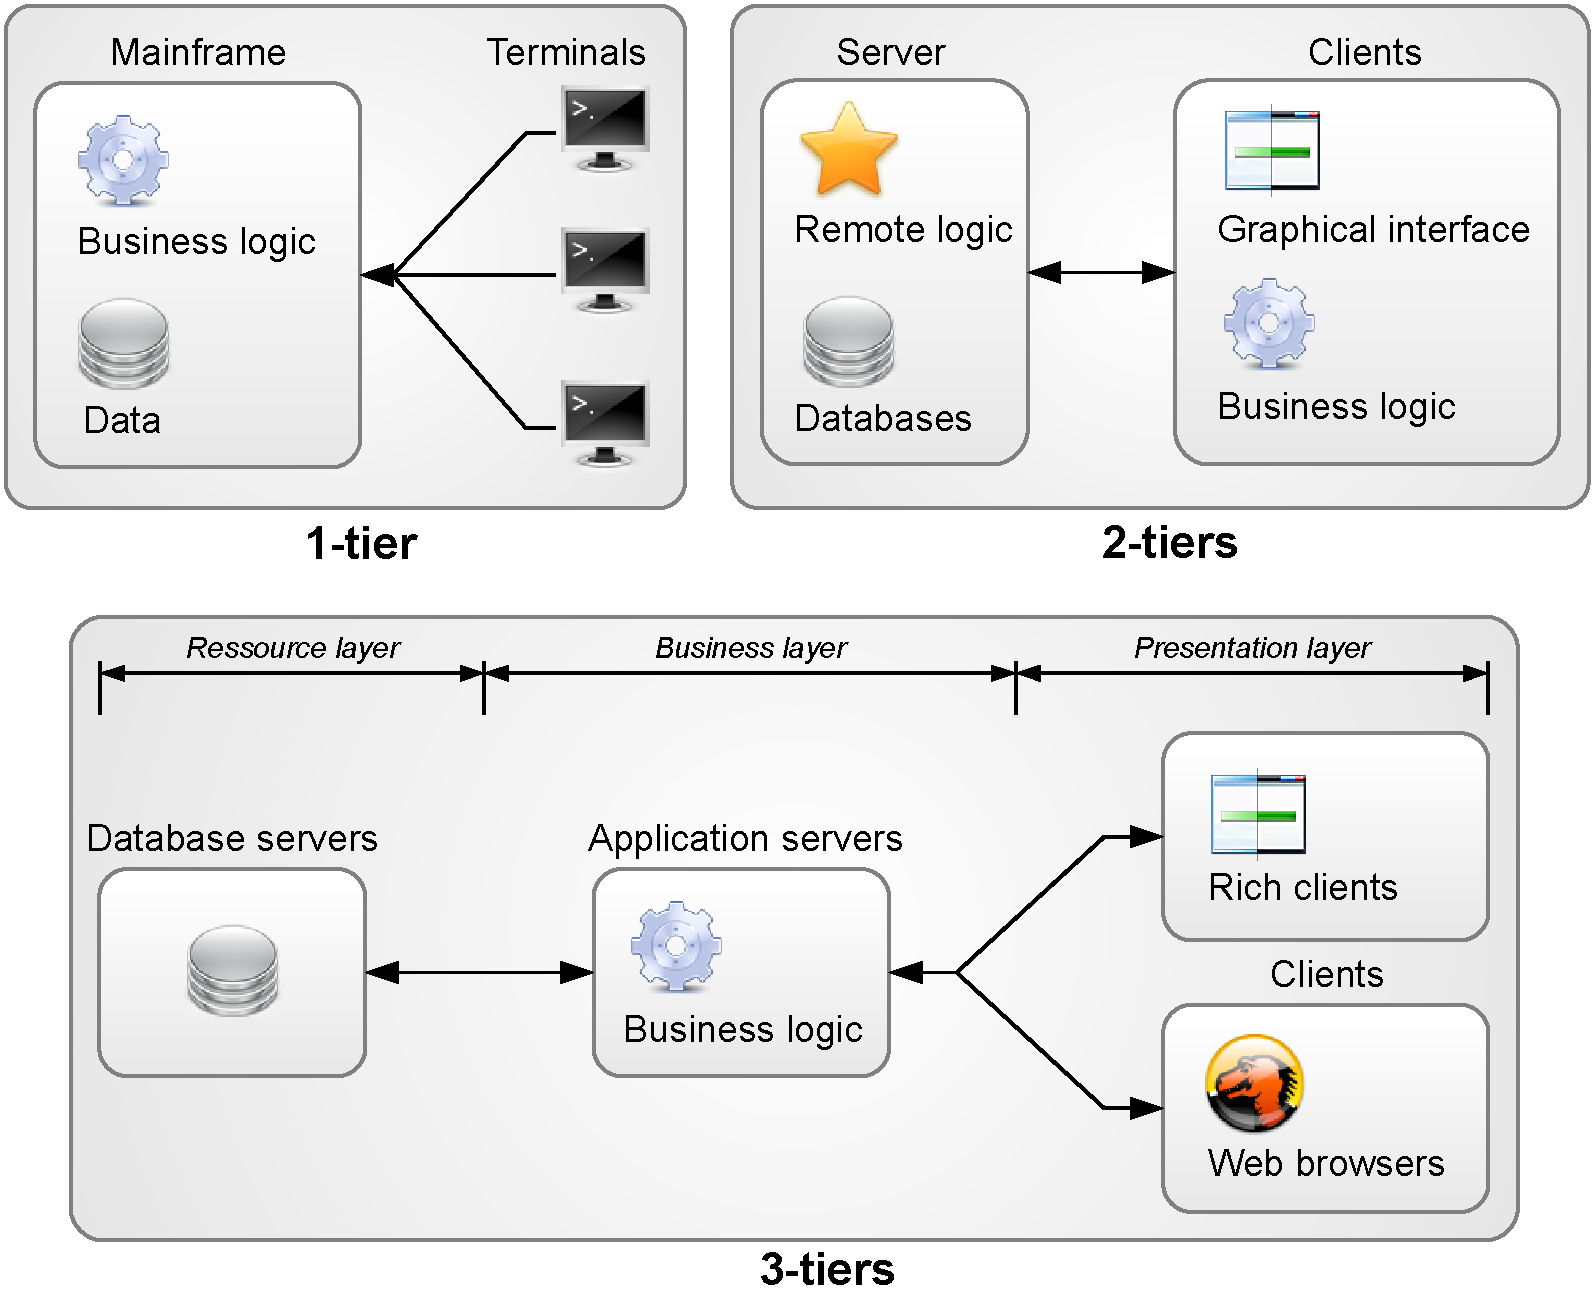
\includegraphics[width=\textwidth]{content/web-services/123-tiers}
    \caption{Overview of typical 1-tier, 2-tiers and 3-tiers architectures.}
    \label{fig:123-tiers}
\end{figure}

From an architectural point-of-view, it is common to differentiate different \emph{tiers} in an application. This is especially true with the generalization of distributed applications as the different tiers can be physically deployed separately \cite{Alonso04}. We briefly present the typical tiered architectures while an overview of them is available in Figure~\ref{fig:123-tiers}.

\paragraph{1-tier (70's -- 80's).}
This type of architecture is highly reminiscent of the early design of enterprise applications of the 70's and has kept being used throughout many developments of the 80's. Those architectures were relying on applications to be deployed on a single physical machine, called a \emph{mainframe}, while end-users would access it through \emph{terminals} over a network (often a proprietary network solution rather than a standards-based one). This type of architecture turned out to be relatively simple to run with simplified maintenance life-cycles as applications were deployed to a single, central machine. It had however a lot of obvious problems, including the need for expensive hardware upgrades to scale up in the number of concurrent terminals or the single-point of failure syndrome.

\paragraph{2-tiers (90's).}
This is also called \emph{client / server} in reference to the decomposition of the application units in server-side and client-side units. Those architectures have been primarily pushed forward by the generalization of relational database management systems exposed through network interfaces, thus providing an application neutral way for applications to store and gather data. The database systems are deployed server-side while the remainder of the application (business logic and visual interface) is client-side. There are variants to this: some computation-intensive tasks can be deported to the server as well. Also, some applications can embed client-side databases. A typical example of this is the support of ``offline modes'' where an application needs to store data when no network connection is available and synchronize it with the server when it becomes available again. Compared to 1-tier architectures, 2-tier applications brought a number of improvements, among which the promotion of standard-based networks as well as normalized data storage and representation systems. Performance-wise, they were also able to introduce clustering of both databases and portions of business logic to handle scalability in the number of clients.

\paragraph{3-tiers and $n$-tiers (end 90's -- 2000's).}
A 3-tiers application comprises the following layers \cite{HW03}.
\begin{itemize}
  
  \item The \emph{resources layer} provides an access to databases, files, network interfaces and legacy applications.
  
  \item The \emph{business layer} provides the core functionalities of applications, no matter how they are accessed. This layer often relies on component technologies (e.g., EJBs\footnote{Enterprise Java Beans}, see \url{http://java.sun.com/products/ejb/}).
  
  \item The \emph{presentation layer} exposes the applications to end-users and applications through a rich set of devices and technologies. In a similar fashion as the model--view--controller paradigm, the very same application can be exposed through different presentation interfaces.
  
\end{itemize}
This type of architecture started to become widespread with the advent of database-driven web applications. It pushed the generalization of \emph{application servers} (e.g., JavaEE, .Net Framework or LAMP\footnote{Acronym for Linux, Apache, MySQL and PHP / Perl / Python (this is not strict as other technologies can be used as replacements).} solutions) that embed the business logic, with the database storage being often delegated to another server. In turn, the presentation layer is accessed through web browsers which are light and generic display devices. Those applications can still be accessed from desktop applications, now called \emph{rich clients} by contrast to web browsers being considered as \emph{thin clients}. The term ``$n$-tiers'' refers to a finer-grained decomposition of an application architecture than 3-tiers. For example in the business layer, a purchase order management component may rely on a remote payment processing component.

\paragraph{Integration placeholders.}
Enterprise integration can be performed:
\begin{itemize}

	\item \emph{horizontally}, by integrating assets from the same tier (e.g., integrating data from heterogeneous customer-centric databases), and
	
	\item \emph{vertically}, by allowing the components from one tier to access to an upper or lower tier (e.g., a payroll management component accessing a relational database).

\end{itemize}
Integrating such assets would be easy in a perfect world where data representation and application interfaces would be uniform. The reality is of course very different as an information system present some of the following sources of heterogeneity: platforms (including operating systems, hardware architectures and execution platforms), databases systems and programming languages.

As an organization evolves, it periodically changes its technological standards, resulting in the need to  integrate new and legacy systems. For example a warehouse management application may have been developed a few years back using the \emph{Delphi} programming platform while new systems need to be developed in Java. Such legacy systems are often kept ``as-is'' since rewriting them has significant costs (e.g., development and training of employees) without necessarily resulting in practical benefits (e.g., the ``old'' application already fulfills the needs). \\

Systems that facilitate both horizontal and vertical enterprise applications integration are called \emph{middlewares}. The next section provides an overview of them.

% ........................................................................... %

\subsection{Middlewares}

% ........................................................................... %

In this section, we review some common middleware families. We also expose the limitations of conventional middlewares. The role of a middleware goes beyond just bridging heterogeneous software artifacts: it hides some of their inherent complexity (much like a \emph{Facade} does in object-oriented programming \cite{Gamma95}). A middleware can provide some development-time infrastructure (e.g., developer tools) and runtime infrastructure (e.g., deployed execution and monitoring components). We give a few examples of middlewares families \cite{Alonso04,HW03}. The platforms that are based on middleware technologies rarely support only a single family. Full-stack application servers such as the ones that provides the JavaEE specification implement much of the following ones.

\begin{figure}[htbp]
    \centering
    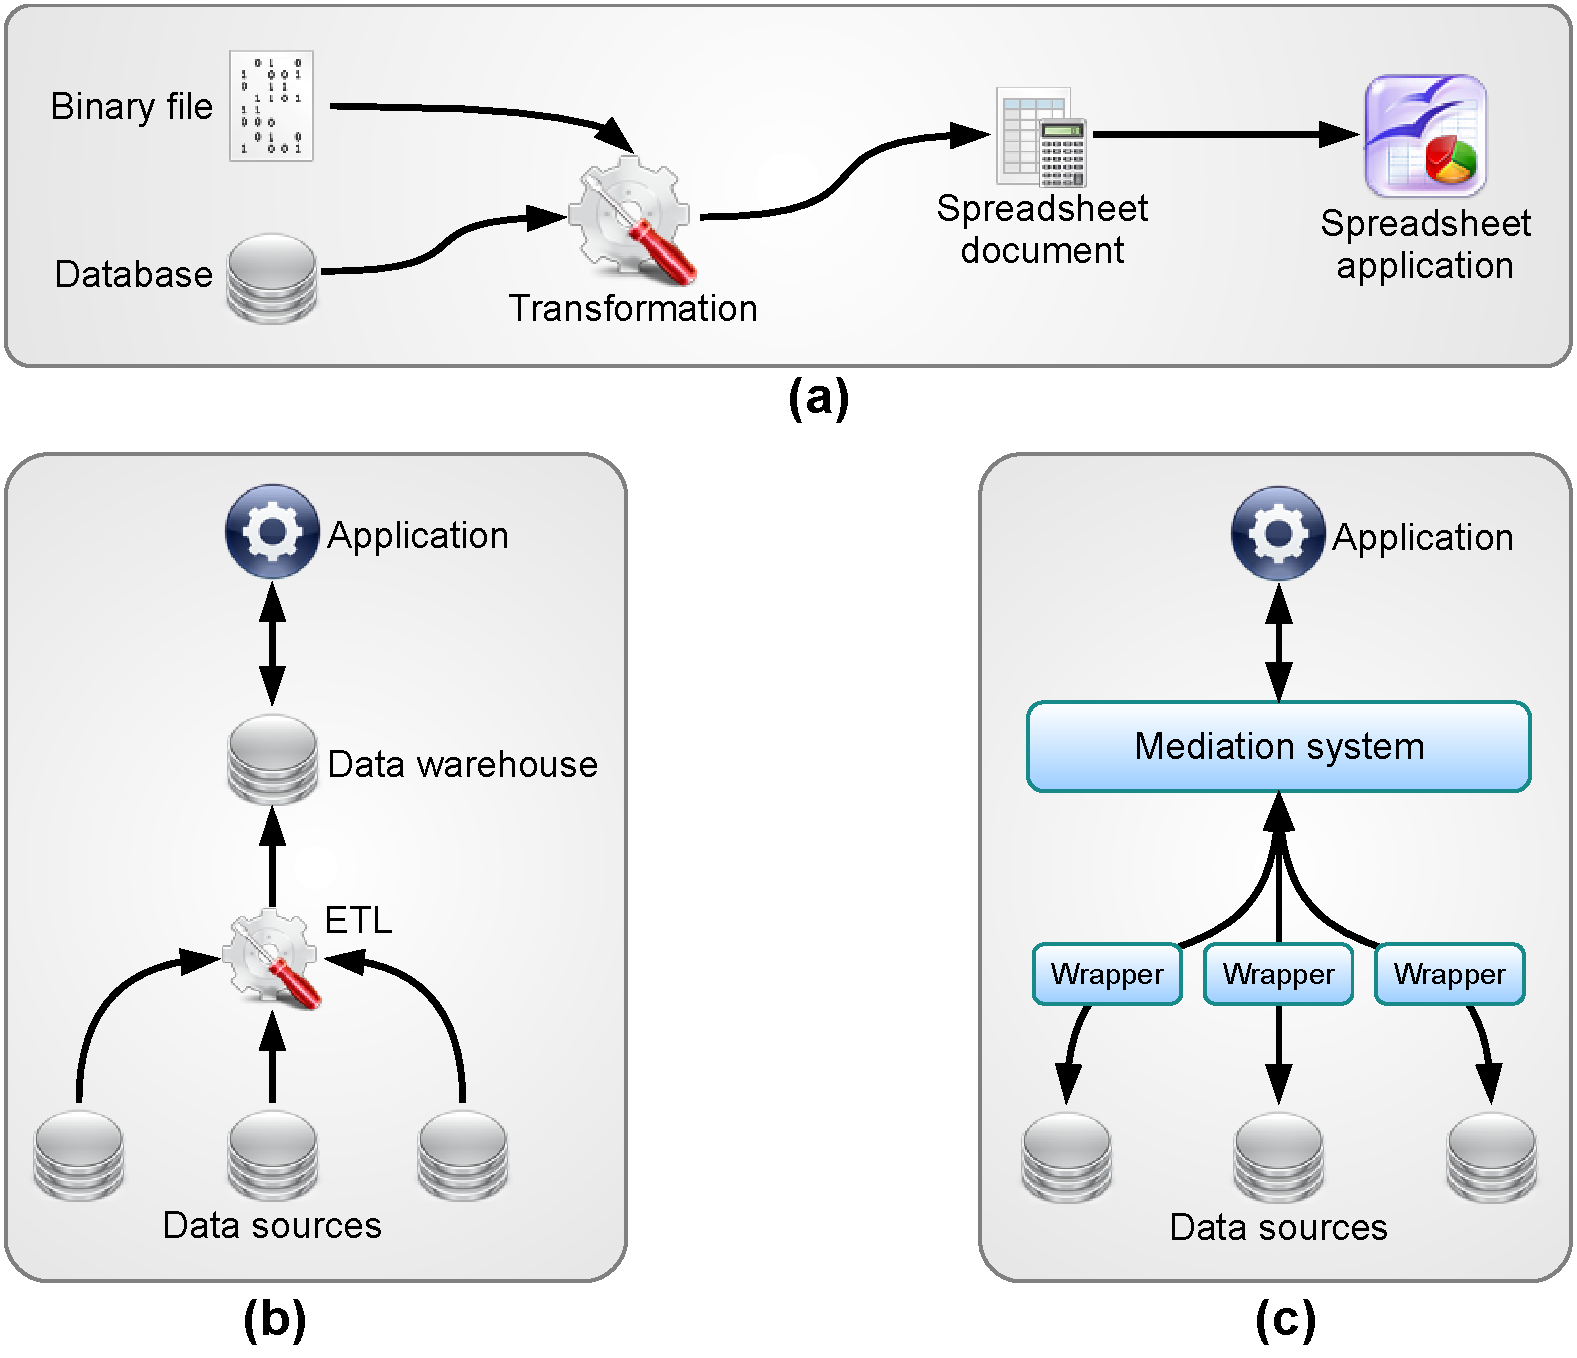
\includegraphics[width=\textwidth]{content/web-services/data-integration}
    \caption{Different approaches for data integration.}
    \label{fig:data-integration}
\end{figure}

\paragraph{Data integration.}
Applications physically store their data in files, databases, relational databases and so on. Several approaches exist, and we illustrated them on Figure~\ref{fig:data-integration}. The first one is to adapt the data from one or more applications so that another one can process it (Figure~\ref{fig:data-integration}(a)). An example would be to extract some data from a spreadsheet document and a relational database and transfer to another application. This involves creating ad-hoc transformation components (e.g., scripts or XSLT transformers). The other approach to data integration is to integrate data sources as heterogeneous, distributed relational databases. In this case there are two ways of achieving it.
\begin{enumerate}

	\item Materialized approaches use ETL\footnote{Extract, Transform and Load} tools that pull data from several relational database sources, normalize/transform it, then finally push it to \emph{data-warehouses} (Figure~\ref{fig:data-integration}(b)).
	
	\item Virtual approaches (Figure~\ref{fig:data-integration}(c)) use techniques and concepts such as \emph{global-as-view} and \emph{local-as-view} where the data is exposed by the mean of queries over the sources (see \cite{Ullman00,Lenzerini02} for an overview and \cite{ChawatheGHPUW94,LevyRO96,LattesR00,HalevyIMMST04} for implementation-related discussions).

\end{enumerate}

\begin{figure}[htbp]
    \centering
    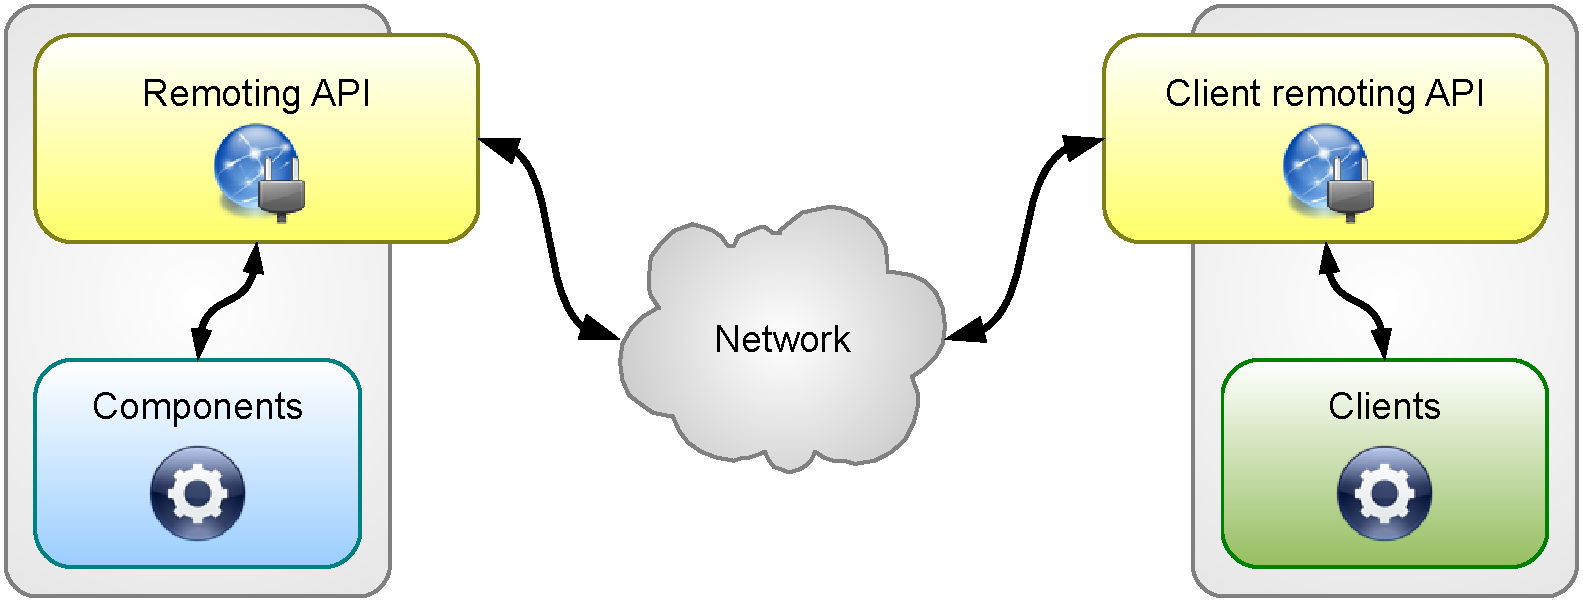
\includegraphics[width=\textwidth]{content/web-services/rpc-middleware}
    \caption{RPC-style middleware.}
    \label{fig:rpc-middleware}
\end{figure}

\paragraph{Remote procedure calls (RPC).}
They allow applications to communicate through regular \emph{procedure / function / method} calls of programming languages. Such a call looks like a normal, local invocation of some application code, but in reality, the actual code that is executed runs on a remote system. To do that, RPC middlewares encode the call parameters in a message that is sent over the network to the remote machine that will run the actual code. Once it has been executed, a response message is sent back to the invoking application with a return value being encoded inside the message. An illustration is provided on Figure~\ref{fig:rpc-middleware}. The preparation of the message (either for performing the call or returning the value) is called \emph{marshaling}. Similarly, the decoding of the message (either on the remote server or the invoker side) is called \emph{unmarshaling}. RCP middlewares have been implemented for a lot of languages and platforms. Examples include distributed components such as EJBs (remote session beans) or Microsoft DCOM.
  
\begin{figure}[htbp]
    \centering
    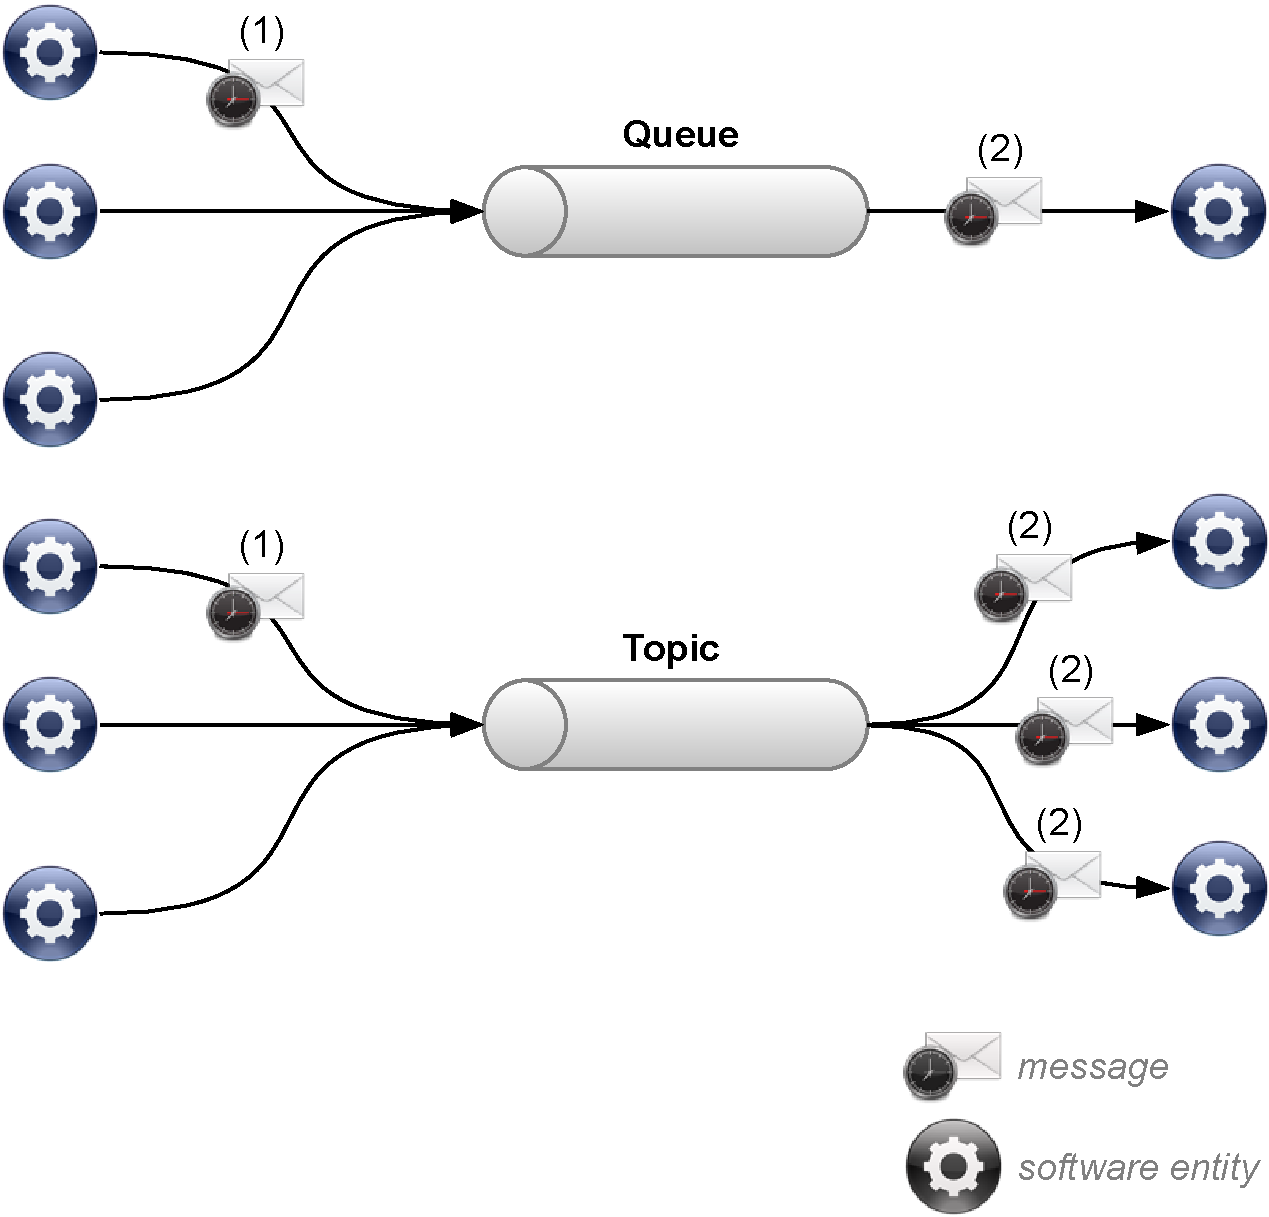
\includegraphics[width=0.8\textwidth]{content/web-services/messaging-middleware}
    \caption{Messaging middleware.}
    \label{fig:messaging-middleware}
\end{figure}
  
\paragraph{Message-oriented middlewares (MOM).}
They allow the communication between applications through asynchronous messages. By contrast to RPC middlewares, the messages do not cary ``function call'' semantics as they are rather general purpose documents exchanged between the systems. A MOM is responsible for collecting and routing messages. It also ensures their integrity, and that the messages are not being lost. Quality of service requirements are generally available, with priorities and validity expiration dates being the two most common in use. A MOM is also able to transform the message contents. This is useful when a message needs to be routed to an application that does not understand the initial message data format.
Two message basic communication patterns are found in MOM (see Figure~\ref{fig:messaging-middleware}): \emph{message queues} provide $n$-to-$1$ communication between $n$ message emitters and one receiver while \emph{message topics} allow broadcasting messages between $n$ emitters and $m$ receivers. An example specification of a MOM is the Java Messaging System (JMS).
  
\paragraph{Object request brokers (ORB).}
They allow clients to delegate the discovery and binding processes of components that match programmatic interfaces. The broker will select the best component according to the criteria it has been configured for, and will provide the clients with objects without them knowing what their concrete implementations are. To do that, an ORB relies on directories of components. Corba (\url{http://www.corba.org/}) is an example of a middleware comprising ORB technology.

\paragraph{Transaction monitors (TP).}
They ensure the coordination of distributed components as part of transactional processes. Relational database management systems have efficient support for transactions on data manipulation, hence it is often natural to rely on them for transactional behavior in applications. This is however not always possible when different business logic components have to be assembled as each of them may not rely on the same database. Those systems usually implement variants of the three-phases commit protocol \cite{SkeenS83}. An example TP is the Java Transactional API (JTA).
  
\begin{figure}[htbp]
    \centering
    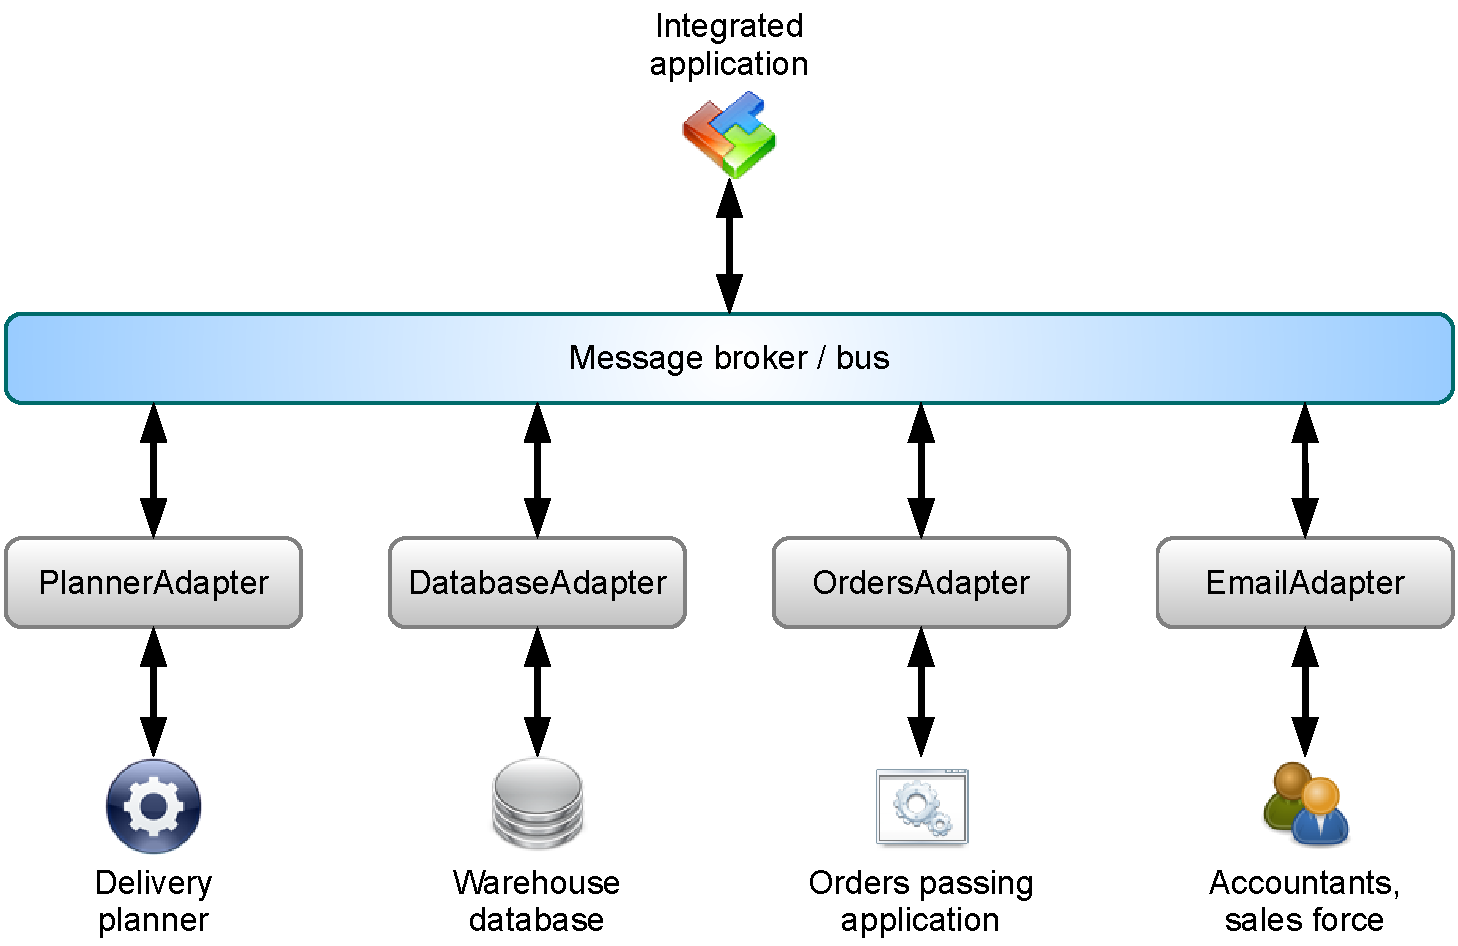
\includegraphics[width=\textwidth]{content/web-services/eai-scenario}
    \caption{Enterprise application integration using a message broker / bus.}
    \label{fig:eai-scenario}
\end{figure}

\paragraph{Example.}
We give an example of an enterprise application integration on Figure~\ref{fig:eai-scenario} where the business process of the purchase orders management is handled through a set of existing applications. Each application is connected through an adapter to a message-oriented middleware, called a \emph{messages bus}. Each message is routed (and possibly transformed) to other entities (e.g., a message sent by the orders passing application for asking goods availability is delivered to the warehouse database adapter). Each adapter is using diverse forms of middleware to bridge the bus and the application. For example the warehouse database adapter can use an ODBC connection to deal with the underlying database, while the delivery planner adapter may use RPC to communicate with the plannification system.

\paragraph{Limitations of conventional middlewares}
The ``conventional'' middlewares that we saw above all share some common limitations. The first one is probably that a lot of adaptation components have to be developed to allow two middleware-based systems to ``talk'' to each other. Another issue is that conventional middlewares are largely centralized \cite{Alonso04}, which limits deployment flexibility and again, requires the development of adapters. As an example, given two RPC frameworks, there is often a need for creating an adapter if they come from different vendors. Worse, even a standard specification is not enough for granting interoperability of systems. A good example is the Java Messaging System (JMS) that defines a standard API for MOM middleware in Java. While every JMS-compliant implementation ensures that an application can be ported from one JMS vendor to another one, there is no requirement on the network protocols and data representation formats, meaning that adapters have to be developed to bridge JMS brokers originating from different vendors.

Things get worse when integration needs to be performed across the boundaries of organizations, as network connectivity issues get added to the (already costly) development of adapters. Indeed, crossing companies firewalls is a serious concern as security need to be preserved, and maintaining such exceptions is complex. Also, a company will rarely trust a partner enough for allowing a direct connexion between their information systems: connectors also need to provide a controlled, coarse-grained interface to the internal information system. Another issue is that in such cases, integration is performed in a point-to-point fashion, something that does not scale well as the number of integrated partners grows \cite{Alonso04}. There is also an inherent lack of flexibility in those approaches as developing adapters and allowing basic connectivity takes time. By contrast, organizations today want to reduce costs, integrate easily with partners and be able to change and outsource some of their assets ``painlessly''.

Web services, and more generally service-oriented architectures have most benefits of the previous middleware families for facilitating application integration. But better, they also solve the mentioned limitations as we will see now.

% ........................................................................... %

\section{Service-oriented computing}

% ........................................................................... %

This section presents service-oriented computing. We start by an overview of service-oriented architectures. We then review the existing web service technologies before looking at service descriptions.

% ........................................................................... %

\subsection{Service-oriented architectures}

% ........................................................................... %

A commonly-accepted definition\footnote{\url{http://webservices.xml.com/pub/a/ws/2001/04/04/webservices/index.html} and \url{http://www6.software.ibm.com/developerworks/education/wsbasics/wsbasics-ltr.pdf}} of web services is the following:
\begin{quote}
\textsl{
Web services are a new breed of Web applications. They are self-contained, self-describing, modular applications that can be published, located, and invoked across the Web. Web services perform functions, which can be anything from simple requests to complicated business processes... Once a Web service is deployed, other applications (and other Web services) can discover and invoke the deployed service.
}
\end{quote}\

Service-oriented architectures (SOA) form the new wave of information systems \cite{PTDL07,PH07}. The key idea of SOA is to turn the data sources and applications in an enterprise system into  distributed units referred to as \emph{services}. Each service is self-described and it is expected to fulfill a very focused set of coarse-grained functionality requirements (e.g., a payroll processing service is not expected to also handle warehouse provisioning). They can then be assembled to realize applications and business processes. Services provide standard-based, platform-neutral interfaces that hide the implementation details. Also, the services should be autonomous with little dependencies to each other. This means that SOA promotes the loose coupling of services that are used for performing application integration of heterogeneous assets. The loose-coupling comes from both the fact that services are autonomous and that they use open standards for their external access (interfaces and data exchange formats).\\

While approaches with similar goals had been developed before the advent of web services (e.g., Corba, distributed components, ...), they bring some novelty \cite{Alonso04}. SOA are indeed often associated with web services as the core mean to realize them. Instead of re-inventing new interface specifications and data encoding means, they directly use widespread, ubiquitous standards such as XML or HTTP. The entry ticket to those technologies is rather low compared to previous approaches, which makes it possible to reuse legacy applications, hide their implementation (including the languages and platform choices) and integrate them with other applications also exposed as services. Another significant improvement in terms of application integration is that SOA blur the traditional boundaries of information systems. Indeed, integrating the information systems of different organizations has traditionally been a costly, largely ad-hoc process \cite{EAA02}, as information systems rarely rely on the same technological choices (e.g., languages, platforms) and normative choices (e.g., data representation formats, schema). Technologies such as web services naturally cross networks without having to develop network-specific bridges (e.g., virtual private networks) and as such, they make it ``natural'' to integrate the heterogeneous information systems of different organizations.\\

\begin{figure}[htbp]
    \centering
    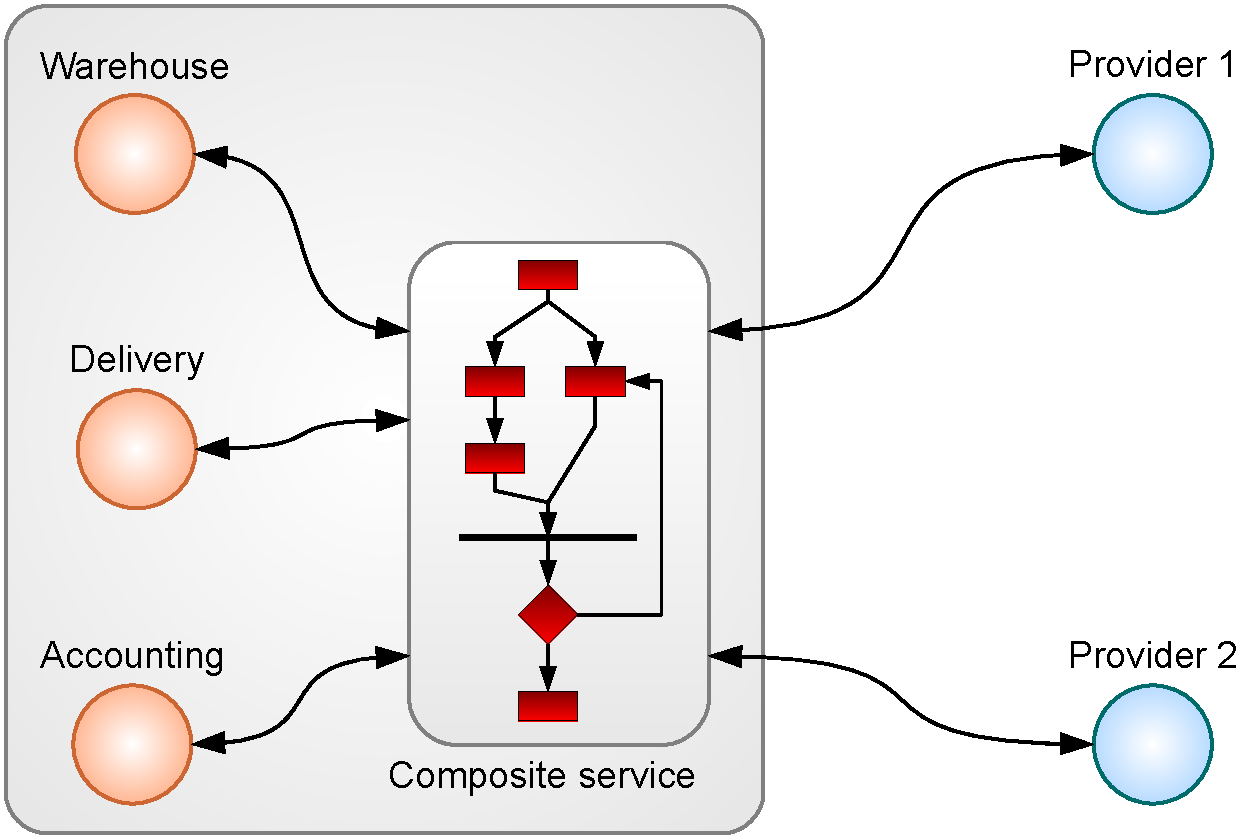
\includegraphics[width=\textwidth]{content/web-services/soa-composition-scenario}
    \caption{A SOA composition scenario.}
    \label{fig:soa-composition-scenario}
\end{figure}

We give an example of a simple service-oriented architecture on Figure~\ref{fig:soa-composition-scenario}. Three in-house services are provided: a warehouse management service, a delivery service and an accounting service. Each of them is an interface to larger applications and data sources and may well have been implemented using different technologies. There are also two external services of providers. A composite service is created by using an orchestration described by a BPEL process (which is not detailed on the figure). When a purchase order is received, it first checks with the warehouse for availability. If not, a quote is asked to each provider for provisioning the warehouse with the cheapest offer. Once this is done, goods are removed from the warehouse for delivery and the payment is delegated to the accounting.
%
In this example, it is possible to externalize the accounting of the organization very quickly: all that is needed is that the accounting provider offers a service with a compatible interface (or more realistically with minimal adaptation required). This is by itself a significant improvement over traditional integration across enterprise information systems.

% ........................................................................... %

\subsection{Technologies}

% ........................................................................... %

We now give an overview of the main web services technologies.

\paragraph{XML-RPC.}
XML-RPC is the first form of web services to have appeared. Defined in \cite{DW98}, it is a small and simple specification for performing RPC-style communications between systems. As the name suggests, the marshaling and unmarshaling of the invocations are done using XML for data representation. The marshaled messages are conveyed using the HTTP protocol (HTTPS can be used for secure point-to-point communications). Both the limited data types and the general minimalism in XML-RPC have facilitated its widespread adoption.

\paragraph{SOAP.}
SOAP \cite{MGMH+03} is a standard protocol defined by the W3C for exchanging XML-based messages between web services and their requesters. It builds on top of widespread existing standards such as XML, URI, HTTP and SMTP. Basically, a SOAP message is an XML document that acts as an envelope for the content being sent. In turn, a SOAP message is meant to be transported over various kind of protocols, the most used being HTTP / HTTPS. While the usual expected alternative is the \emph{Standard Mail Transfer Protocol} (SMTP), real-world applications have been using IIOP (from Corba), XMPP (Jabber open instant messaging) or even JMS (\emph{Java Messaging System}) to route SOAP messages. SOAP messages can be used either to simulate RCP-style communications, or document-style communications which are analogous to asynchronous messaging systems.

\begin{figure}[htbp]
    \centering
    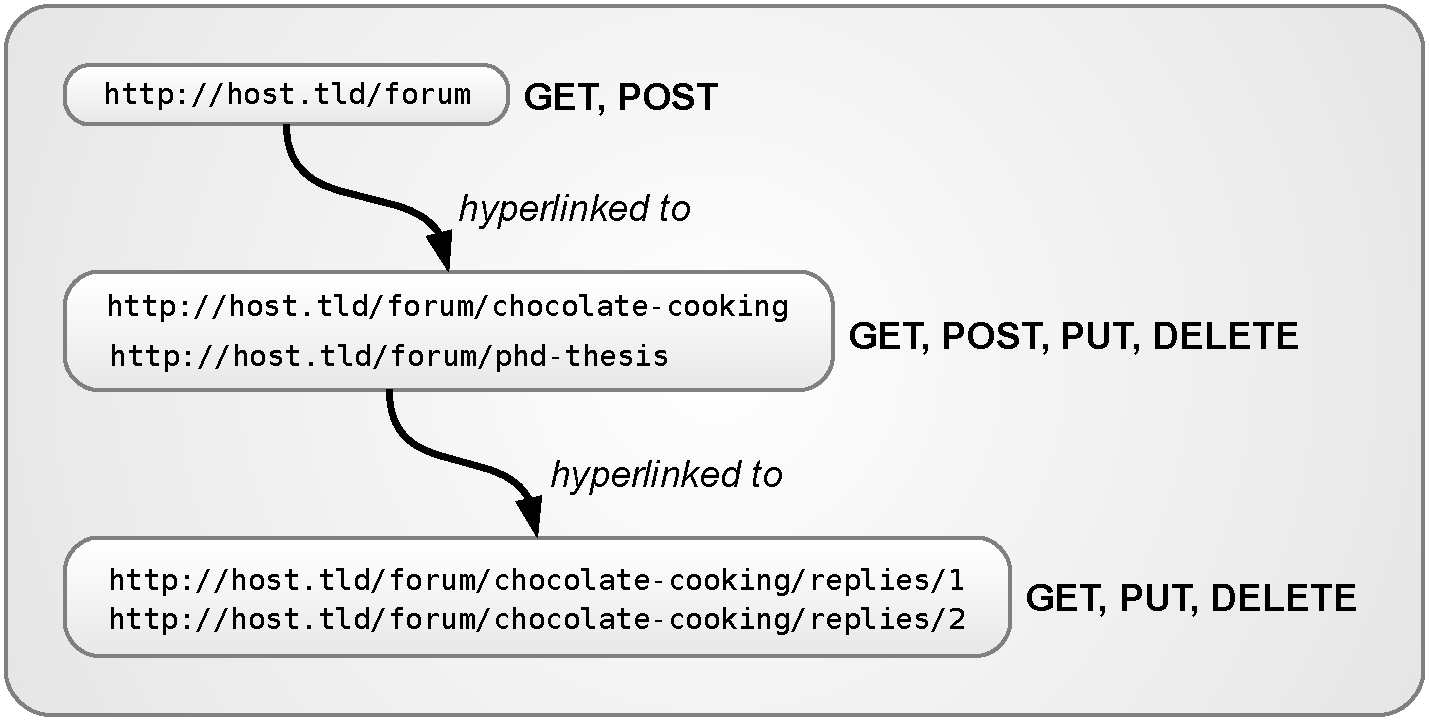
\includegraphics[width=\textwidth]{content/web-services/restful-forum}
    \caption{A \emph{RESTful} forum application.} 
    \label{fig:rest-forum}
\end{figure}

\paragraph{REST.}
The concept of REST\footnote{REST stands for \emph{\textbf{RE}presentational \textbf{S}tate of \textbf{T}ransfer}.}-style services first appeared in \cite{RTF00}. It is not a formal specification of a technology for building web services. Rather, it is an architectural style for building web services that emphasizes the semantics of both the HTTP protocol and the \emph{Universal Resource Identifiers} (URIs).
The core concept behind REST is that applications expose \emph{resources} that are accessible through URIs over the HTTP protocol. A resource may have several \emph{representations}, i.e., it may use different data encodings (e.g., XML, CSV, plain text) to accommodate different requesters. The resources can be \emph{hyperlinked} with each other and manipulated through a limited set of \emph{verbs}: the HTTP protocol methods (\textsf{GET}, \textsf{POST}, \textsf{PUT} and \textsf{DELETE}, see \url{http://www.w3.org/Protocols/rfc2616/}). As such, resources provide a \emph{uniform interface} to applications \cite{RTF00}.
We give an example of a \emph{RESTful}\footnote{Widely-used jargon for touting an application as being designed using the REST philosophy.} forum application on Figure~\ref{fig:rest-forum}. Hyperlinked resources can be manipulated by a HTTP software agent (e.g., for fetching message threads or posting a reply).

\begin{figure}[htbp]
    \centering
    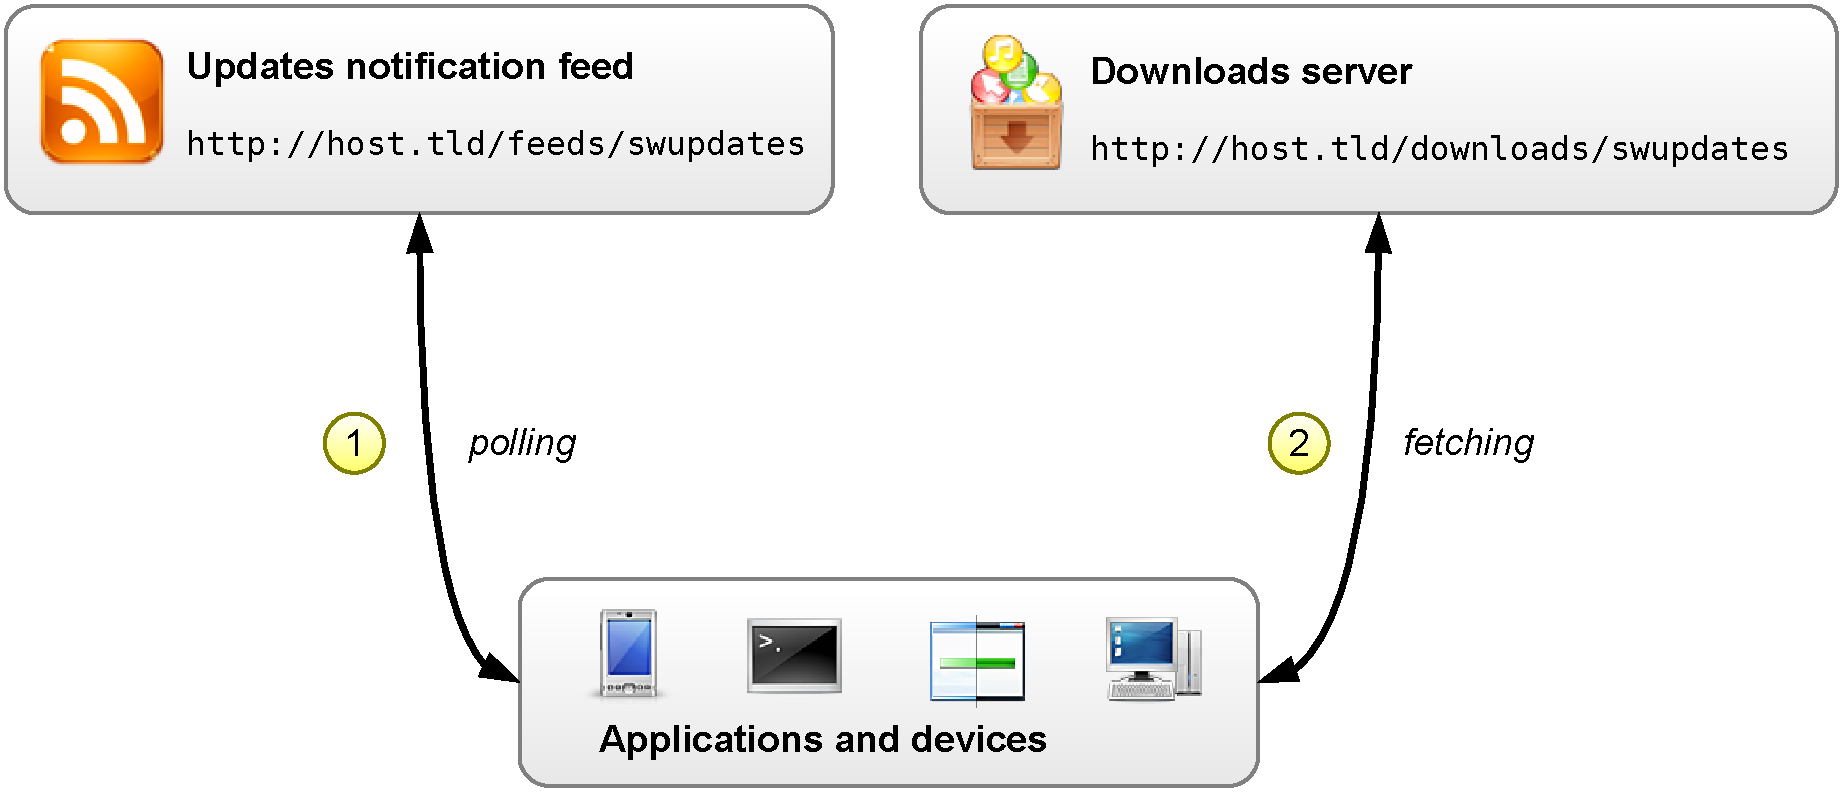
\includegraphics[width=\textwidth]{content/web-services/syndication-scenario}
    \caption{A simple software updates notification and distribution scenario based on syndication.} 
    \label{fig:syndication-scenario}
\end{figure}

\paragraph{Syndication feeds.}
Syndication web services have become increasingly popular with the rise of collaborative online applications such as blogs, wikis and podcasting. They provide resources called \emph{feeds} to notify \emph{subscribers} of events (e.g., a new blog post is available). The service does not directly notifies the subscribers of changes. Rather, it provides a URL-accessible resource which is updated when needed. Subscribers poll the resource for changes on a periodical basis. Two XML-based specifications are currently competing. An example is given on Figure~\ref{fig:syndication-scenario} where a feed is made available for publishing software update notifications.

% ........................................................................... %

\subsection{Service description and discovery}

% ........................................................................... %

We now briefly review standards and specifications for describing static web services interfaces and discovering them.

\paragraph{Static interface.}
The \emph{Web Services Description Language} (WSDL) \cite{ECFC+01} is an important add-on to SOAP-based web services. It provides a description of the static interface of such a service, much like IDL can be used in component technologies. As such, it specifies the operations supported by the service, the data schemas, and the binding information used to communicate with the service such as the transport protocol being used (ex: HTTP) and the location of the service (in the case of HTTP as a transport protocol, a URL). The messages that can be exchanged between a requester and a service are described using XML Schema (\url{http://www.w3.org/XML/Schema}).

A WSDL document can be used to bind to a SOAP-based service in two ways: either client invocation source code can be generated from the WSDL, or the binding can be performed dynamically at runtime. The latter case is especially possible with dynamic and reflexive languages such as \emph{Java} or \emph{Ruby}, by using the \emph{Proxy} design-pattern \cite{Gamma95}. Once either the static or dynamic binding has been performed, the service can be invoked.

\paragraph{Registries.}
The \emph{Universal Description, Discovery and Integration (UDDI) protocol} (see \url{http://www.uddi.org/}) provides a way for repositories to contain service functional and non-functional descriptions. Ultimately, a client interested in a given discovered service is able to obtain its WSDL description and bind to it after having found it. Another proposal for services repositories can be found in \emph{ebXML} (see \url{http://www.ebxml.org/}).

\paragraph{WS-*.}
Several specifications are gravitating around the SOAP web services stack \cite{HMBBFC+06}, often referred to as ``WS-*'' specifications. Most of them are actually irrelevant with no practical adoption in real-world use-cases \cite{WS-standards}. Among the very few relevant ones we have:
\begin{itemize}
  
  \item WS-Security (\url{http://docs.oasis-open.org/wss/v1.1/}), a specification for end-to-end preservation of the messages confidentiality and authenticity
  
  \item WS-Addressing (\url{http://www.w3.org/Submission/ws-addressing/}), which defines a standard representation for endpoint references and routing schemes (useful for correlation in stateful web services)
  
  \item WS-Policy (\url{http://www.w3.org/Submission/WS-Policy/}), a standard representation of quality of service requirements (e.g., security, message-encoding optimizations, ...)
  
  \item WS-Reliability (\url{http://docs.oasis-open.org/wsrm/ws-reliability/v1.1}) is useful for ensuring that messages are properly delivered in contexts that are not point-to-point communications between the service provider and its requesters
  
  \item WS-Coordination (\url{http://docs.oasis-open.org/ws-tx/wscoor/2006/06/}) and WS-Transaction (\url{http://dev2dev.bea.com/pub/a/2004/01/ws-transaction.html}) allow the coordination of web services.
  
\end{itemize}

The next section presents the model of business protocols \cite{FTBB} that serves as a foundation of this thesis work as it is suitable for describing the external behavior of a service with respect to the conversations it supports.

% ........................................................................... %

\section{Business protocols}

% ........................................................................... %

Static interface descriptions such as WSDL are essential for facilitating the use of web-service based technologies. There is however a strong need for abstractions of a higher-level than just ``data formats and message names''. As such, there is a consensus over the need for also specifying the dynamic interface of services \cite{PTDL07,PH07,ws_cacm_special_issue}. In particular, the externally-observable behavior of a service is important for avoiding invalid conversations between a service and its requesters. For example, a service may offer to add goods to a shopping cart and make a payment. A WSDL document of such a service would give the related message names (e.g., \emph{addGoods} and \emph{pay}) as well as their XML schema. This is clearly insufficient as for instance, paying before adding goods is most often not a valid business process.

This section first recalls the business protocol model and its usefulness. It then presents protocol-based analysis before providing a discussion.

% ........................................................................... %

\subsection{Model}

% ........................................................................... %

The model of business protocols of \cite{FTBB,BBFC04,BCT-CAISE03,KBBB+04} is the foundation of the work being presented in this thesis. This model captures all of the conversations that a service supports, i.e., the set of ordered message exchanges that are valid (e.g., a purchase order should not be exchanged before an authentication message). As such, it provides an abstraction for capturing a service external behavior, allowing potential requesters to know how to avoid generating invalid conversations, which is by itself a significant enhancement compared to having ``just'' a WSDL description. The model is based on state-charts as it is commonly accepted as a suitable model for describing behaviors, but alternatives could have been used as well such as Petri-nets or abstract BPEL (the later capture the operations orderings in a BPEL process).\\

\begin{figure}[htbp]
    \centering
    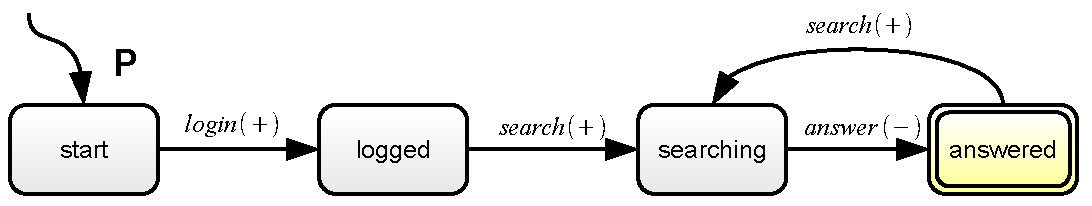
\includegraphics[width=\textwidth]{content/web-services/business-protocol}
    \caption{A business protocol of a search engine.} 
    \label{fig:business-protocol}
\end{figure}

As an example, Figure~\ref{fig:business-protocol} shows a business protocol of a search engine. States represent the various stages a service may go through while transitions are triggered when a message is received or sent. There is a unique initial state and many final states. In this protocol, conversations start with the service receiving a \texttt{login} message (the polarity $(+)$ is used to indicate that the message is incoming). Following that, a search can be performed and the results can be retrieved through repeatable sequences of \texttt{search} -- \texttt{answer} messages (again, the polarity $(-)$ is used for messages that are emitted by the service). The \textsf{answered} state is final: every conversation that ends in this state is said to be valid. By contrast, an invalid conversation would be $\mathtt{search} \cdot \mathtt{login} \cdot \mathtt{answer}$. Finally, it should be noted that state names do not have much importance in the model as conversations are about messages being exchanged.\\

Business protocols can be useful in several analysis contexts, both at development and runtime \cite{FTBB,BBFC04,BCT-CAISE03,KBBB+04}. Conformance checking is useful for a service provider to check if the actual implementation of a service meets a specification which can be either provided to clients (e.g., in the documentation), or imposed from standards (e.g., RosettaNet PIPs \cite{ROSETTANET}). Another one is for a requester to check that its own client protocol is compatible with a service, and if it is not, perform some adaptations so as to accommodate the service protocol to avoid errors. Finally, there are cases were a service needs to be replaced (e.g., failures, business-driven need for changing partners, etc). Replaceability analysis is useful so that a new service can be used as an alternative with minimal impacts on the existing requesters. Especially, it helps in identifying the potential mismatches at the protocol level so that adapters can be created. As such, both compatibility and replaceability analysis can be interesting as part of a service discovery process. In this work, we are interested in protocol-based compatibility and replaceability analysis that we outline hereafter.

% ........................................................................... %

\subsection{Protocol analysis}

% ........................................................................... %

Business protocols allow to perform fine-grained types of compatibility and replaceability analysis to see if (and how) two services can have interactions based on their protocols (compatibility), or if a service can be replaced transparently by another one for its current requesters (replaceability). Several classes of both compatibility and replaceability have been defined.
\begin{itemize}

	\item \emph{Partial compatibility} between two protocols $\mathcal{P}_1$ and $\mathcal{P}_2$ implies that at least one conversation can be carried out between two services implementing these protocols.

  \item A protocol $\mathcal{P}_1$ is \emph{fully compatible} with $\mathcal{P}_2$ if $\mathcal{P}_2$ can support all message exchanges that $\mathcal{P}_1$ can generate (the inverse is not necessarily true).
  
  \item \emph{Protocol equivalence} occurs when two protocols support exactly the same conversations.
	
	\item \emph{Protocol subsumption} occurs when a protocol supports at least all of the conversations of another one.
	
	\item \emph{Protocol replaceability w.r.t. a client protocol} occurs when a protocol $\mathcal{P}_1$ can replace a protocol $\mathcal{P}_2$ when interacting with a client protocol $\mathcal{P}_c$ if every valid conversation between $\mathcal{P}_2$ and $\mathcal{P}_c$ is also a valid conversation between $\mathcal{P}_1$ and $\mathcal{P}_c$.
	
	\item \emph{Protocol replaceability w.r.t. an interaction role} is similar to the previous one. It occurs when a protocol $\mathcal{P}_1$ can replace a protocol $\mathcal{P}_2$ if $\mathcal{P}_1$ behaves like $\mathcal{P}_2$ when $\mathcal{P}_2$ behaves as an interaction role $\mathcal{P}_r$.

\end{itemize}

Those analysis classes are characterized by using a set of protocol operators.
\begin{itemize}

	\item The \emph{intersection} operator computes the common conversations that two services support.
	
	\item The \emph{parallel composition} operator computes the common interactions that can take place between two services.
	
	\item The \emph{difference} operator computes which conversations are supported by a given service, but not by a second one.

\end{itemize}

\begin{figure}[htbp]
    \centering
    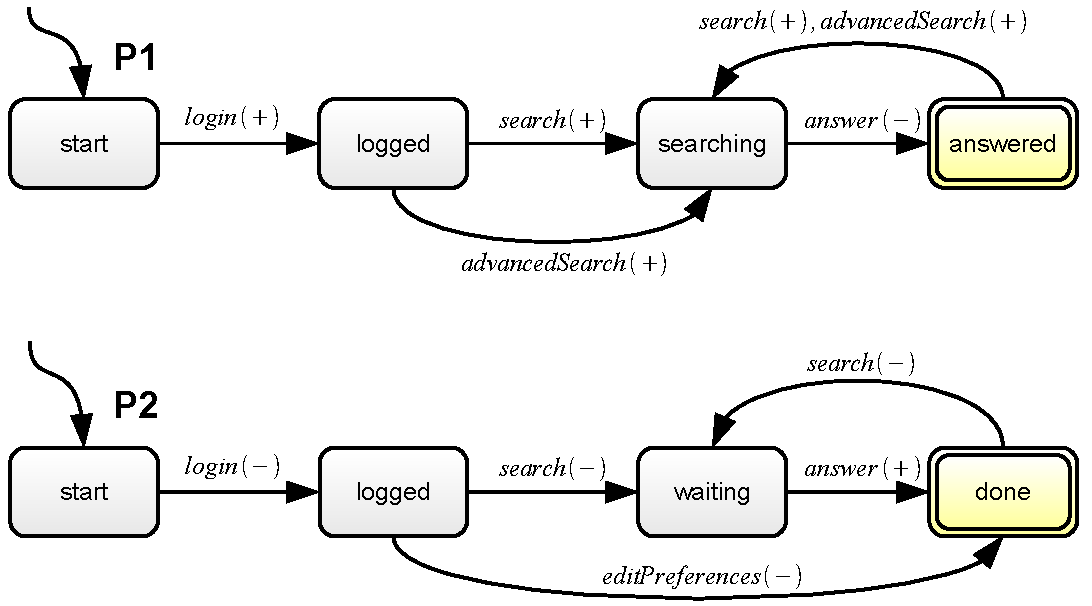
\includegraphics[width=\textwidth]{content/web-services/business-protocol-analysis}
    \caption{Two business protocol for illustrating analysis.} 
    \label{fig:business-protocol-analysis}
\end{figure}

As an example, two services are partially compatible as long as their parallel composition yields a non-empty protocol (i.e., at least one conversation is supported). This is the case between the protocol $P$ of Figure~\ref{fig:business-protocol} and $P_2$ of Figure~\ref{fig:business-protocol-analysis}. They are however not fully compatible as $P_2$ can generate some conversations that $P$ cannot support (e.g., $P$ does not support \texttt{editPreferences} messages).

In terms of protocol replaceability, the protocol $P$ of Figure~\ref{fig:business-protocol} can be replaced by the protocol $P_1$ of Figure~\ref{fig:business-protocol-analysis}. Indeed, there is protocol subsumption of $P$ by $P_1$. The two  protocols are however not equivalent as $P$ does not support \texttt{advancedSearch} messages: $P$ cannot replace $P_1$.

% ........................................................................... %

\subsection{Discussion and related work}

% ........................................................................... %

The following discussion first reviews common model families as business protocols opted for a state-based model. Notions such as orchestration, choreography and models for service abstractions are then briefly reviewed. Finally, research projects for web services life-cycle management are mentionned.

\paragraph{Model families.}
We consider the following three families: state-based models, activity-based models and rule-based models. 
State-based models can be found in a variety of contexts, mainly for describing behavioral abstractions of a system. In particular, the UML models family \cite{UML} contains several of them, acting as different ``facets'' over the representation of a system depending on the type of information that is to be captured (i.e., the general system behavior, the system behavior in a specific choreography, etc). We briefly recall the most important of them.
\begin{itemize}

    \item Collaboration diagrams
    allow to represent the message exchanges between several (distributed) entities. Arrows are drawn between the entities, carrying both a message and number. The number (part of a total order) is used to define the messages chronology of the collaboration that is being modeled.

    \item Sequence diagrams
    are similar to the collaboration diagrams except that they use \emph{lifelines} to denote when the object representing the entities are instantiated and discarded. Messages are exchanged between those lifelines, optionally having a number as in the case of collaboration diagrams. Indeed, the message exchange arrows are usually sorted vertically by chronological order.

    \item Statecharts
    capture all of the possible states of a given entity. The transitions between states are triggered on events (for example a message is received).

\end{itemize}

Activity-based models have been used to represent systems in an executable form (e.g, workflow management systems \cite{aalst98application}). States represent activities, and the transitions are triggered when the activities are finished. Each entity is given a \emph{swimlane}, and an activity belongs to the swimlane of the executing entity. In some of those models, the transitions can carry data flows.

Rule-based systems \cite{Forgy79,Forgy82} define behavior through a set of \emph{rules}. A rule is triggered when a given \emph{event} occurs, or when a given \emph{condition} is met. The rule then defines an action which is executed. Rule-based systems have been widely used where the systems behavior need frequent updates from domain experts writing the rules in domain-specific languages.

We chose to base our model upon the state-machine formalism. Indeed, it is commonly used to model the behavior of systems, due to the fact that it is simple and intuitive. Activity-based models are more suitable for creating executable models. Finally, rule-based models are a natural fit for complex decision-making systems where the logic must be frequently updated (e.g., by business analysts, accountants, etc.). They are however less suitable for describing behaviors.

\paragraph{Models for service abstractions.}
Research on web services has naturally lead to various models being proposed for capturing different types of abstractions. A discussion on modeling web services interactions has been proposed in \cite{TB-WWV06} and is further discussed in \cite{BSF06}. An approach for web services interfaces was defined in \cite{DBACTH05}. A model with similar goals as timed protocols had been introduced in \cite{berardi03finite}, but the timing constraints defined in the model have yet to be taken into account. A language for web services choreographies called \emph{Chor} has been proposed in \cite{QZCY-WWW07} as a simplification of WS-CDL.
WS-CDL (see \url{http://www.w3.org/TR/ws-cdl-10/}) is the reference specification for choreographies. Tools leveraging WS-CDL for facilitating development of SOA systems are currently emerging \cite{KangWH07}. BPEL also offers \emph{abstract process} for describing the externally observable behavior of a service composition. Lesser-known alternatives to BPEL include YAWL \cite{AalstADH04,AalstH05}, a general-purpose workflow language that has support for web services.

All of those approaches share many similarities with this work and the base model for business protocols of \cite{FTBB}. Surprisingly, little work has been done on timing abstractions. Also, those works do not provide a fine-grained range of compatibility and replaceability analysis classes, which makes our work original. Finally, business protocols and WS-CDL are complementary, not competing proposals.

\paragraph{Life-cycle management research projects.}
The \emph{ServiceMosaic project} \cite{BCTPM06-SM} aims at developing a model-driven framework for web service life-cycle management. It has a CASE tools set for supporting the service development life-cycle that includes facilities for modeling, analyzing, discovering and adapting web service models \cite{BCTPM06-SM,NezhadSBCPT07}. The work presented in this thesis is part of this project. ServiceMosaic is presented in larger details in chapter~\ref{chap:protocols-project}.

The \emph{Self-Serv} project was the precursor of the larger-scope ServiceMosaic project: \cite{ShengBDM02,BenatallahDM02,BenatallahSD03}. The goal of Self-Serv was to allow for rapid composition of web services through a declarative approach. The execution of the obtained composite services was made in peer-to-peer, dynamic environment.

The project called \emph{Astro} is another platform for the life-cycle management of web services \cite{TrainottiPCZLBBT05}. It features several contributions in the area of business requirements and verification, service synthesis and composition, and semantic web services. While it shares some similarities with ServiceMosaic (e.g., adaptation, supporting composition, Eclipse-based implementation), it focuses more on orchestration models (based on BPEL) than choreographies (e.g., the business protocol that a service supports). There is also no model discovery component such as the protocol discovery from execution log tools suite that ServiceMosaic provides \cite{Motahari-NezhadSBC07}. Finally, some works in Astro consider timing abstractions \cite{KazhamiakinPP06}. However, the work that is presented in this paper mainly reuses well-known timed automata model-checking techniques in service-based compositions. As we will see later, our approach makes a novel use of timed automata for obtaining the decidability and closure of protocol operators, not for performing straightforward, traditional model-checking. \\

While business protocols provide \emph{temporal constraints} (i.e., the messages ordering), they do not provide \emph{timing constraints} (e.g., a payment must be performed at most 48 hours after having purchased). This thesis revisits the concepts of business protocols modeling and analysis and enhances them using timing constraints. The result is a model that supersedes business protocols with added timing constraints and adapted analysis techniques. As we  established a link between our extended model and timed automata \cite{RADLD94} to obtain theoretical results on the time-aware analysis of protocols, we present them in the next chapter.

% ........................................................................... %


\chapter{Timed automata}
\label{chap:timed-automata}
% ........................................................................... %

We give here some background knowledge on timed automata, a model that has been extensively used in the field of real-time model checking, and that will be useful for the remainder of this work. We begin with an overview of the model before focusing on the common problems (e.g., closure under complementation and reachability analysis). We then review some classes of timed automata that are interesting for this work, before finishing with model checking tools. \\

This will turn out to be useful later in the remainder of this work. Indeed, our approach for analyzing services business protocols completely depends on the closure under intersection and complementation in timed automata. It  also depends on the ability to perform location reachability analysis using a model checking tool.

% ........................................................................... %

\section{Overview}

% ........................................................................... %

We start with an overview of the model of timed automata, including its semantics. We then turn our attention to the ``classic'' problems such as closure under intersection or language inclusion.

% ........................................................................... %

\subsection{Model and semantics}

% ........................................................................... %

Timed automata were introduced in \cite{RADLD94} as an extension of classical automata \cite{Hopcroft79} to model real-time systems. Some preliminary works appeared in \cite{RACC94}. We start by an informal example before going through the formalization and semantics of the model.

\begin{figure}[htbp]
    \centering
    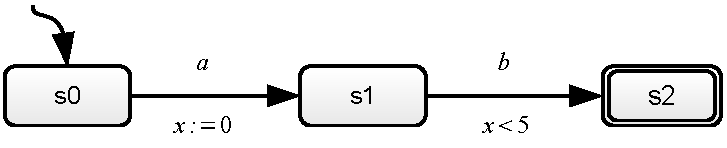
\includegraphics[width=0.9\textwidth]{content/timed-automata/sample-ta}
    \caption{A sample timed automaton $A$.}
    \label{fig:sample-ta}
\end{figure}

\paragraph{Extension of automata with clocks.}
We take as an example the timed automaton $A$ depicted on Figure~\ref{fig:sample-ta}. At first sight, $A$ is much like a ``normal'' automaton: it has locations (e.g., $s_0, s_1$ and $s_2$) as well as switches with labels over the alphabet $\Sigma = \{ a, b \}$. There is one initial location $s_0$ while $s_2$ is an accepting location. Hence, an (untimed) word $a \cdot b$ can be recognized by $A$ while words such as $a \cdot a$ or $b \cdot a$ cannot. Timing constraints are added in $A$ by making use of a clock $x$ which is a continuous variable over the set of real-valued numbers $\Rpos$. Of course, a timed automaton can have more than one clock. $A$ recognizes the set of timed words $a \cdot b$ such that $b$ is recognized at most 5 units of time after $a$. To do that, the clock $x$ is reset to $0$ when the automaton switches from the location $s_0$ to $s_1$ on the symbol $a$. Again, a switch can reset an arbitrary number of clocks. Initially, every clock is set to $0$ and then, they grow synchronously as time evolves. Clocks can be used in constraints attached to the switches, called guards, and that can enable or disable a switch depending on how those boolean functions over the clocks evaluate. Here, the clock $x$ is used in the guard of the $b$-labeled switch so that $b$ cannot be recognized when $(x \geq 5)$ is true.\\

Time elapses in the locations, while the switches are instantaneous. It is also possible to bound the time spent in the locations by defining clocks constraints called \emph{invariants}, which can be used to force switches to be fired before the invariants conditions become violated. Indeed, it is a requirement that time can always elapse in the locations. Timed automata recognize \emph{timed words} which are sequences in which a non-negative real value is attached to each symbol. For example $w = (a, 0) \cdot (b, 1)$ is a timed word where $b$ has been recognized 1 unit of time after $a$. More precisely, a timed word over an alphabet $\Sigma$ is a sequence $(a_0,t_0) \cdot (a_1, t_1) \cdots (a_n, t_n)$ such that $a_i \in \Sigma$,  $t_i \in \Rpos$ and  $t_0 < t_1 < \cdots < t_n$.

\paragraph{Clocks valuations.}
In what follows, we reuse the same notations as in \cite{RADLD94,RA98}.
Given a set of clocks $X$ with their values being in $\Rpos$, a clocks valuation $v$ for $X$ is a function $X \longrightarrow \Rpos$ that associates to each clock $x \in X$ its value $v(x)$. The set of clocks valuations for $X$ is written $\Rpos^X$. The set of clocks constraints over $X$ is $\mathcal{C}(X)$, built using boolean combinations of atomic constraints of the form $x \;\#\; c$ with $x \in X$, $\;\#\; \in \{=, \neq, <, \leq, >, \geq \}$ and $c \in \Q$. $\mathcal{C}_{\prec}(X)$ is the restrictions of $\mathcal{C}(X)$ where the clocks constraints are of the form $x < c$ or $x \leq c$. A clocks valuation $v$ satisfies an atomic constraint $(x \;\#\; c)$ if and only if $(v(x) \;\#\; c)$ is true. This allows to check whether a complete constraint $g$ can be satisfied by a clocks valuation $v$, denoted as $v \models g$. Given $d \in \Rpos$, $v' = v + d$ is the clocks valuation such that $v'(x) = v(x) + d$ for each $x \in X$. Also, given a subset of clocks $r \in X$, $v' = [r \leftarrow 0]v$ is the clocks valuation such that $v'(x) = 0$ if $x \in r$ and $v'(x) = v(x)$ if $x \in X \setminus \{ r \}$.

\begin{definition}[Timed automata] \cite{RADLD94,RA98}
  
A timed automaton $A$ is a tuple $A = (\Sigma, L, L^0, L^f, X, I, E)$ where:
\begin{itemize}

    \item $\Sigma$ is the \emph{alphabet},

    \item $L$ is a finite set of \emph{locations} (or states),

    \item $L^0 \subseteq L$ is the set of \emph{initial locations},

    \item $L^f \subseteq L$ is the set of \emph{final locations} (or accepting states),

    \item $X$ is a finite set of clocks,

    \item $I : L \rightarrow \mathcal{C}_{\prec}(X)$ associates an \emph{invariant} to each location

    \item $E \subseteq L \times \mathcal{C}(X) \times \Sigma \times 2^X \times L$ is a finite set of switches (or switches) $e = (l, g, a, r, l') \in E$ from $l$ to $l'$, where $g$ is the guard, $r$ is the set of clocks to be reset and $a$ is the label.

\end{itemize}
\end{definition}

A timed automaton $A$ recognizes timed words that are sequences of the form $(a_1, t_1) \cdot (a_2, t_2) \cdots (a_n, t_n)$ where given $i \in \{1, 2, \cdots, n\}$, $a_i \in \Sigma$ is a symbol from the alphabet and $t_i \in \Rpos$ is the time at which $a_i$ is recognized by $A$. The set of timed words recognized by a timed automaton $A$ is the timed language denoted as $L(A)$.

\paragraph{Semantics.}
The semantic of a timed automaton $A$ is defined using an (infinite) timed \emph{labeled transitions system} (LTS). Each state of the LTS is a pair $(l, v) \in L \times \Rpos^X$, called a \emph{configuration}, where $l$ is the current location in $A$ and $v$ is a clocks valuation. There are two types of transitions: \emph{action transitions} (labeled with a symbol of $\Sigma$) and \emph{time transitions} (labeled with a real-valued duration). More precisely, the semantic of $A = (L, L^0, L^f, X, I, E, \Sigma)$ is given by the LTS $\mathcal{S}_A = (S, s_0, \rightarrow, \Sigma)$ where:

\begin{itemize}

    \item $S = L \times \Rpos^X$,

    \item $s_0 = (l_0, v_0)$ with $l_0 \in L^0$ and $v_0(x) = 0$ $\forall x \in X$,

    \item $\rightarrow$ is the transition relation:
    \begin{itemize}

        \item action transitions: $(l, v) \stackrel{a}{\longrightarrow} (l', v')$ if and only if there exists
        $e = (l, g, a, r, l') \in E$ such that $v \models g$, $v' = [r \leftarrow 0]v$ and $v' \models I(l')$

        \item time transitions: if $d \in \Rpos$ then $(l, v) \stackrel{d}{\longrightarrow} (l, v + d)$ if and only if $v + d \models I(l)$.

    \end{itemize}

\end{itemize}

The LTS $\mathcal{S}_A$ starts from an initial state made from an initial location and each clock set to $0$. Then, either instantaneous action transitions occur (possibly resetting some clocks), or time transitions allow the clocks to grow synchronously. The executions over $\mathcal{S}_A$ match the timed words that can be recognized by $A$ when they start from the initial state of $\mathcal{S}_A$ and they can reach a final state.\\

\begin{figure}[htbp]
    \centering
    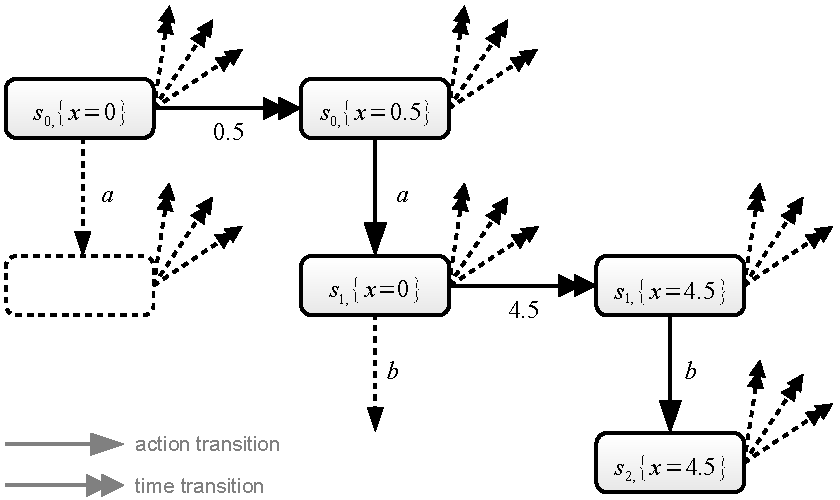
\includegraphics[width=\textwidth]{content/timed-automata/semantic-lts}
    \caption{The LTS $\mathcal{S}_A$ associated to the timed automaton $A$ of Figure~\ref{fig:sample-ta}.}
    \label{fig:semantic-lts}
\end{figure}

Let us consider again $A$ defined on Figure~\ref{fig:sample-ta} and its semantic LTS $\mathcal{S}_A$ which is depicted on Figure~\ref{fig:semantic-lts}. $(s_0, 0) \stackrel{1}{\longrightarrow} (s_0, 1) \stackrel{0.25}{\longrightarrow} (s_0, 1.25) \stackrel{a}{\longrightarrow} (s_1, 0) \stackrel{0.1}{\longrightarrow} (s_1, 0.1) \stackrel{b}{\longrightarrow} (s_2, 0.1)$ is a valid execution over $\mathcal{S}_A$ which recognizes the timed word $(a, 1.25) \cdot (b, 1.35)$ of the timed language $L(A)$.

% ........................................................................... %

\subsection{Classic problems}

% ........................................................................... %

We now review some classic problems for timed automata. They are summarized in Table~\ref{tab:ta-common-problems}.

\begin{table}[htbp]
\centering
\begin{tabular}{|p{7cm}|p{5cm}|}

    \hline

    \textit{Problem} &
    \textit{Results} \\

    \hline \hline

		Union & Closed \\ \hline
		
		Intersection & Closed \\ \hline
		
		Projection & Closed \\ \hline
		
		Complementation & Not closed \\ \hline
		
		Language inclusion & Undecidable \\ \hline
		
		Language equivalence & Undecidable \\ \hline
		
		Universality & Undecidable \\ \hline
		
		Language emptiness / reachability analysis & \textsc{PSPACE-Complete} \\ \hline

\end{tabular}
\caption{Classic problems for (general) timed automata \cite{RADLD94}.}
\label{tab:ta-common-problems}
\end{table}

\paragraph{Closure properties.}
Closure of timed automata under the following operators has been studied in \cite{RADLD94}: union, intersection, complementation and projection\footnote{Projection allows to map a timed language from one to another with a different alphabet (symbols that are not mapped are replaced by $\varepsilon$).}. Union and intersection are based on extensions of the classical procedures on automata \cite{Hopcroft79}. The closure under union and intersection is relatively easy. Closure under union comes from the fact that timed automata are indeterministic and support more than one location. Intersection is similar. The problematic non-closure under complementation is a consequence of indeterminism, as a timed word may have more than one execution. The proof is based on the observation that a timed word can have an execution ending in a final location and one in a non-final location, making it impossible to construct the complement like for untimed automata.

\paragraph{Timed language inclusion, equivalence and universality.}
We briefly introduce these three decision problems.
%
Given two timed automata $A$ and $A'$, the \emph{timed language inclusion problem} refers to checking if $\mathcal{L}(A) \subset \mathcal{L}(A')$. Similarly, the \emph{timed language equivalence problem} refers to checking if $\mathcal{L}(A) = \mathcal{L}(A')$. Finally, the \emph{universality problem} refers to checking whether a timed automaton $A$ defined over an alphabet $\Sigma$ is able to recognize all of the possible timed words over $\Sigma$.
%
These problems require the ability to complement timed automata. As an example, checking whether $\mathcal{L}(A) \subset \mathcal{L}(A')$ reduces to checking for the timed language emptiness of the automaton $A' \cap \overline{A}$. Unfortunately, timed automata are not closed under complementation, making these problems undecidable.
%
Checking for the emptiness of a timed language is a \textsc{PSPACE-Complete} problem. This problem is also referred to as the \emph{location reachability} problem (i.e., a timed language is empty if no final location can be reached.

\begin{figure}[htbp]
    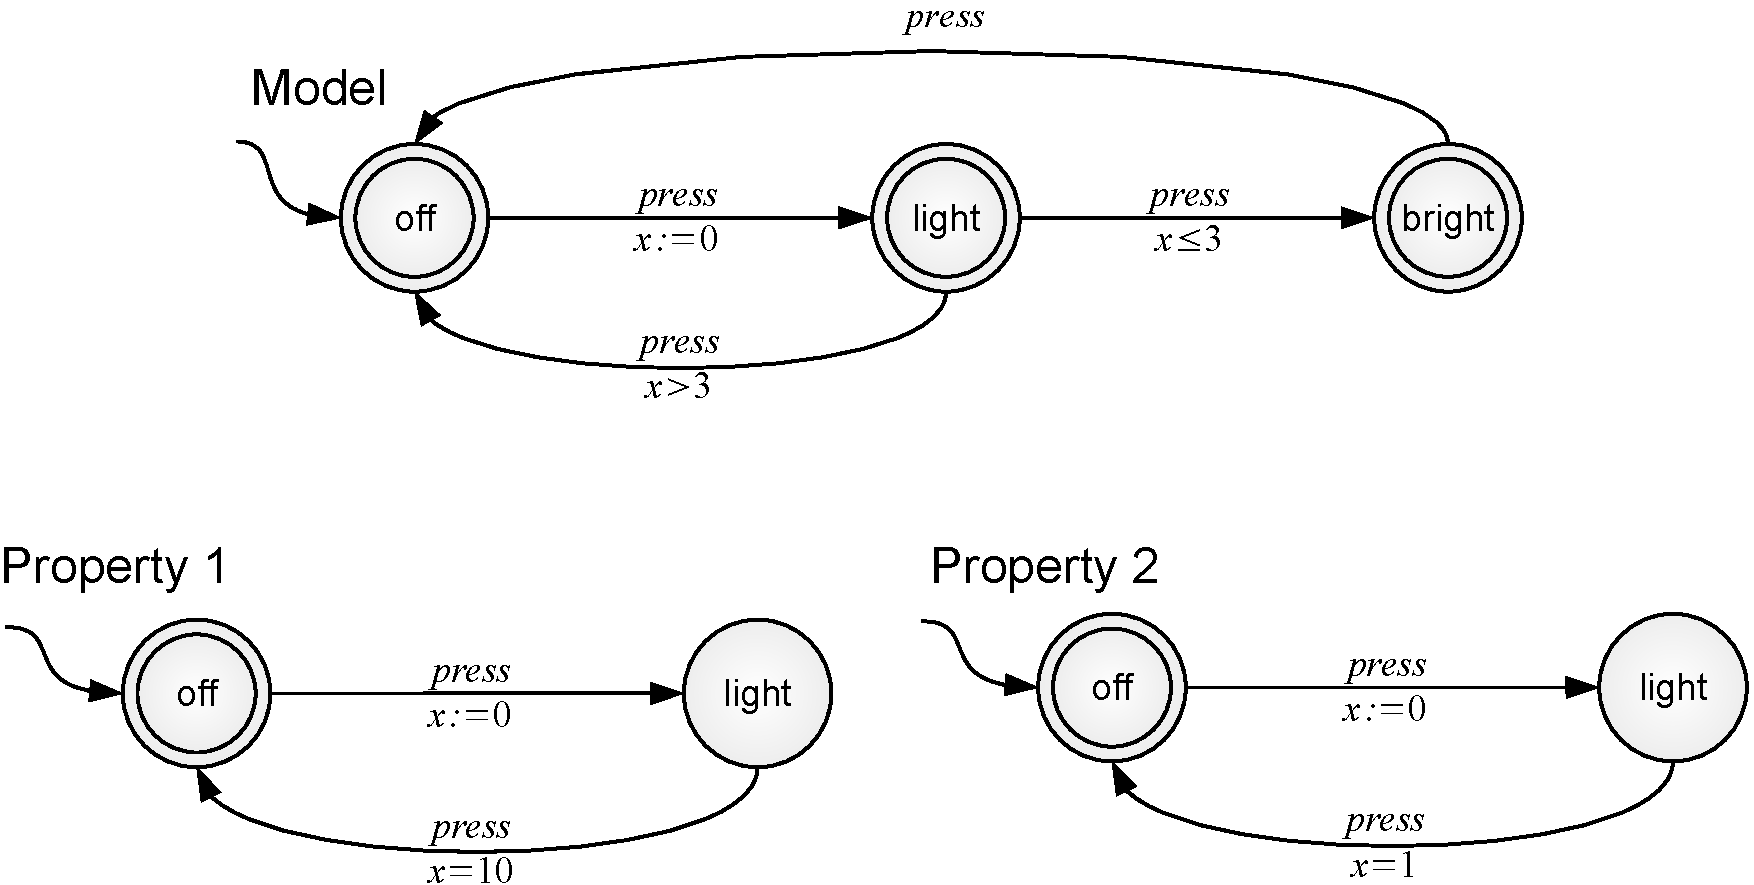
\includegraphics[width=\textwidth]{content/timed-automata/light-verification-inclusion}
    (\textit{model from} \url{http://www.cis.upenn.edu/~alur/Talks/sfm-rt-04.ppt})
    \caption{A model checking example that reduces to state reachability analysis.}
    \label{fig:light-verification-inclusion}
\end{figure}

\paragraph{Verification through test automata.}
In this case, the property to verify is expressed as a timed automaton, referred to as a \emph{test timed automaton}. The verification is performed by a reduction to a reachability / emptiness analysis. We give an example on Figure~\ref{fig:light-verification-inclusion}. The system that is modeled is a light controller. The light is initially turned off, and pressing it will turn it on. However, if the button is pressed twice quickly (within at most 3 units of time), then the light will be brighter. Finally, pressing the button another time will turn the light off.

We express two properties on this system using timed automata. The first one (property one) is used to test whether pressing the button once, then 10 units of time later will turn it off again. This is property that we expect to be satisfied by the modeled system. In turn, we do not expect the second property to be true: when pressed quickly twice, the light should not be turned off.

Model-checking through the mean of test automata is not always the best option, as verification reduces to a timed language inclusion checking problem. While checking for timed language emptiness is decidable (yet \textsc{PSPACE-Complete}), the non-closure under complementation is problematic. We will see later in this chapter that some classes of timed automata do not suffer from this issue. Back to the example of Figure~\ref{fig:light-verification-inclusion}, this is possible as the automata are deterministic.

% ........................................................................... %

\section{Classes of timed automata}

% ........................................................................... %

Several classes and extensions of timed automata have been studied. Indeed, the fact that the decision problems seen above are undecidable in the general case motivated such research directions. We summarize here the principal classes and extensions of timed automata that turned out to be useful in the context of this work.
%
Table~\ref{tab:ta-classes-decidability} summarizes the results regarding the timed language inclusion and emptiness checking problems, while Table~\ref{tab:ta-classes-expressiveness} details the results on expressiveness.
%
Further pointers can be found in \cite{RAPM04,RA98,ST03,JOJW04,BL-VAT06}.

\begin{table}[htbp]
\centering
\footnotesize
\begin{tabular}{|p{5cm}|p{4.5cm}|p{2.5cm}|}

	\hline
	
	\textit{Class or extension} &
	\textit{Emptiness checking} &
	\textit{Language inclusion} \\
	
	\hline \hline
	
	  Timed automata &
    \textsc{PSPACE-Complete} &
    Undecidable \\

    \hline

    Deterministic timed automata &
    \textsc{PSPACE-Complete} &
    Decidable \\

    \hline

    Event-clock automata &
    \textsc{PSPACE-Complete} &
    Decidable \\

    \hline

    Robust timed automata &
    \textsc{PSPACE-Complete} &
    Undecidable \\

    \hline \hline

    $\varepsilon$-transitions without clocks resets &
    \textsc{PSPACE-Complete} &
    Undecidable \\

    \hline

    $\varepsilon$-transitions with clocks resets &
    \textsc{PSPACE-Complete} &
    Undecidable \\

    \hline

    Diagonal constraints ($x - y \;\#\; c$)&
    \textsc{PSPACE-Complete} &
    Undecidable \\

    \hline

    Additive constraints ($x + y \;\#\; c$) &
    Decidable for 1 or 2 clocks, open problem for 3 clocks and undecidable starting from 4 clocks \cite{BerDuf-IPL2000} &
    Undecidable \\

    \hline
    
    Constraints of the form $x = 2y$ &
    Undecidable \cite{RADLD94} &
    Undecidable \\
    
    \hline
    
    Constraints with irrational constants &
    Undecidable \cite{Miller00} &
    Undecidable \\

    \hline

    Non-standard ($x := 0$) clocks resets &
    Decidable for $x := c$, undecidable for $x := x -1$ and decidable for $x := x + 1$ if diagonal constraints are not allowed \cite{BDFP04} &
    Undecidable \\
    
    \hline

\end{tabular}
\caption{Emptiness and timed language inclusion checking results for some classes and extensions of timed automata.}
\label{tab:ta-classes-decidability}
\end{table}

\begin{table}[htbp]
\centering
\footnotesize
\begin{tabular}{|p{5cm}|p{7.5cm}|}

    \hline

    \textit{Class or extension} &
    \textit{Observations} \\

    \hline \hline

    Deterministic timed automata &
    Strictly less expressive than timed automata \\

    \hline

    Event-clock automata &
    Indeterministic event-clock automata can always be rendered deterministic while this is not the case for (general) timed automata \cite{RALF94} \\

    \hline

    Robust timed automata &
    Robust timed languages are \emph{open} and their expressiveness is not comparable with the one of timed languages \cite{RAPM04} \\

    \hline \hline

    $\varepsilon$-transitions without clocks resets &
    The silent transitions can be removed \cite{VDPG97} \\

    \hline

    $\varepsilon$-transitions with clocks resets &
    Strictly more expressive than general timed automata: the silent transitions that reset clocks cannot be removed in general \cite{VDPG97,BBVD+99,LSV:07:12} \\

    \hline

    Diagonal constraints ($x - y \;\#\; c$)&
    More concise than timed automata, but not more expressive \cite{BBVD+99} \\

    \hline

    Additive constraints ($x + y \;\#\; c$) &
    More expressive than timed automata \\

    \hline

\end{tabular}
\caption{Expressiveness of some classes and extensions of timed automata.}
\label{tab:ta-classes-expressiveness}
\end{table}

\paragraph{Deterministic timed automata.}
The class of \emph{deterministic timed automata} has been defined in \cite{RADLD94}. It restricts the definition of timed automata by:
\begin{enumerate}
  
  \item allowing only a single initial location, and
  
  \item requiring that given two switches from the same source location having the same input symbol, their guards are disjoint so as to preserve determinism.
  
\end{enumerate}
As such, the timed automaton of Figure~\ref{fig:sample-ta} is deterministic. This is also true for the timed automata depicted on Figure~\ref{fig:light-verification-inclusion}.
Each timed word that is recognized by a deterministic timed automaton has exactly one accepting run over it. Deterministic timed automata form a strict subclass of timed automata (they are less expressive). The problem of the determinization of indeterministic (untimed) automata is decidable \cite{Hopcroft79}. This is however not the case for timed automata \cite{ST03}.

\paragraph{Event-recording timed automata.}
Event-clock automata, and more particularly \emph{event-recording automata} form an interesting class of timed automata \cite{RALF94}. In this model, clocks are assigned to the input symbols. Each time one of symbol is recognized (e.g., $a$), its associated clock is reset (e.g., $x_a$). The time domain $\T$ is the set of positive reals $\Rpos$ augmented with the $\perp$ symbol to denote the fact that a given symbol has not been recognized yet (i.e., every clock is set to $\perp$ initially). The fundamental property in event-recording automata is that the value of clocks only depends on the input word. The consequence of this is that such automata are \emph{determinizable} (i.e., an indeterministic event-recording automaton can always be transformed into a deterministic one that recognizes the same language) and \emph{complementable} (i.e., event-recording automata are closed under complementation). Extensions of event-recording automata can be defined as long as the value of clocks only depends on the input word.

\paragraph{Silent transitions.}
In the case of untimed automata, they do not add to the expressiveness and they can be removed easily \cite{Hopcroft79}. This is however not the case with timed automata, and as we will see later in this thesis, this will be a major issue for the decidability of timed protocol operators, as the model of timed protocols exhibits such transitions. Indeed, allowing silent ($\varepsilon$) transitions in timed automata strictly adds to the expressiveness \cite{VDPG97,BBVD+99,LSV:07:12}. Complex techniques exist to remove the $\varepsilon$-transitions when they do not reset clocks \cite{VDPG97}. However, this is not possible in the general case when they do reset clocks, i.e., there exist switches of the form $l \xrightarrow{\varepsilon, g, \{ x \}} l'$. Of special interest is the notion of \emph{precise actions} defined in \cite{BBVD+99}, as it gives a tool for proving that some timed languages cannot be recognized by a timed automaton without $\varepsilon$-labeled switches. We will leverage this tool when studying the expressiveness of timed protocols.

\paragraph{Other classes.}
Some classes or extensions have different expressiveness levels compared to (general) timed automata. The expressiveness of the class of \emph{Robust timed automata}\footnote{Briefly, a robust timed automaton recognizes  timed words with some fuzziness in the event dates as no real world system can be expected to be as precise as timed automata expectations.} cannot be compared to the one of timed automata \cite{RAPM04}. The classical decidability problems (reachability / emptiness, inclusion) remain unchanged.

The closure and decidability results remain unchanged compared to (general) timed automata in the following cases: constraints of the form $x = 2y$, constraints with irrational constants, and allowing non-standard (i.e., $x := 0$) clocks resets.

In most cases, the emptiness / reachability problem is decidable (yet \textsc{PSPACE-Complete}) despite the language inclusion problem being undecidable because of non-closure under complementation. However, some forms of modified clocks constraints and clocks resets can render it undecidable \cite{BerDuf-IPL2000,RADLD94,Miller00,BDFP04,BBVD+99,LSV:07:12,VDPG97}.

\paragraph{Other formalisms.}
Several formalisms have been introduce to capture timing constraints. Among them, a common abstraction is to define delays with minimum and maximum values on timed transition systems: \cite{HenzingerMP94,MerrittMT91,LynchA92,PnueliH88}.

Petri nets support extensions with timing requirements \cite{petrinets}. \emph{Timed Petri nets} are an extension where a transition can be fired only if its enabling duration is in a certain time window \cite{PMM74}. In turn, \emph{Timed Petri nets} associate to each transition a set of time windows \cite{Ramchandani74}. The tokens that circulate in timed Petri nets are given an age. A transition can then be fired only by tokens whose ages are in one of the time windows of the transition.

Lots of contributions bridging timed automata and timed Petri nets have been made. The work done in \cite{BHR-ICALP2006} is of most interest as it proves that timed Petri nets are not more expressive than timed automata with respect to the language equivalence. It introduces a class called \emph{Read-arc timed Petri nets} which is language-equivalent to timed automata.

\paragraph{Temporal logics.}
They have been traditionally used for formal verification purposes. A temporal logic formula  expresses some form of \emph{qualitative time} property such as \emph{``when the light is off, pressing the button will turn it on''}. To put it another way, temporal logics allow to specify the order of events. However, it is not possible to express \emph{quantitative time} properties such as \emph{``when the light is off and the button is pressed twice in less than 2 seconds, the light will be bright''}.

The purpose of a temporal logic formula is to check wether there exists a path to a state that satisfies the formula in the considered system. Two branches of temporal logics exist:
\begin{enumerate}
  
  \item \emph{linear-time temporal logics} allow reasoning over a single time line, and
  
  \item \emph{branching-time temporal logics} allow reasoning over several time lines.
  
\end{enumerate}
CTL, which stands for \emph{computational tree logic}, is the traditional branching-time logic \cite{ClarkeES86} while LTL (\emph{linear temporal logic}) is the traditional linear-time logic \cite{Pnueli77}.

Both CTL and LTL have been extended to support quantitative time. TCTL (\emph{timed computational tree logic}) \cite{HNSY94} extends the branching-time logic CTL. Similarly, MTL (\emph{metric temporal logic}) \cite{Koymans90} and TPTL (\emph{timed propositional temporal logic}) \cite{AlurH89,AlurH94} extend the linear-time temporal logic LTL to support quantitative time. Some fragments of MTL have been defined to seek better decidability results: as MITL (\emph{metric interval logic}) \cite{AlurFH96}, Safety-MTL \cite{OuaknineW05} and coFlat-MTL \cite{BouyerMOW07}. 

\begin{table}[htbp]
\centering
\footnotesize
\begin{tabular}{|p{3.5cm}|p{9cm}|}

    \hline

    \textit{Logic} &
    \textit{Model-checking problem} \\
    
    \hline
    
    TCTL &
    \textsc{PSPACE-Complete} \cite{AlurCD90,AlurCD93} \\
    
    \hline
    
    \multirow{2}{5cm}{MTL over finite runs} &
    Decidable and non-primitive recursive under the pointwise semantics \cite{OW07} \\
    
    \cline{2--2} &
    Undecidable under the continuous semantics \cite{AlurFH96} \\
    
    \hline
    
    MTL over infinite runs &
    Undecidable under pointwise semantics \cite{OuaknineW06} \\
    
    \hline
    
    TPTL over finite runs &
    Undecidable under the pointwise and continuous semantics \cite{AlurH94} \\
    
    \hline
    
    MITL over infinite runs &
    \textsc{EXPSPACE-Complete} \cite{AlurFH96} \\
    
    \hline
    
    Safety-MTL over infinite runs &
    Decidable but not primitive-recursive under the pointwise semantics \cite{OuaknineW05} \\
    
    \hline
    
    coFlat-MTL over infinite runs &
    \textsc{EXPSPACE-Complete} under the pointwise semantics \cite{BouyerMOW07} \\
    
    \hline
    

\end{tabular}
\caption{Results on the problem of model-checking using timed temporal logics.}
\label{tab:temporal-logics-checking}
\end{table}

The results on the problem of model-checking using timed temporal logics are summarized in Table~\ref{tab:temporal-logics-checking}. The branching-time logic TCTL offers very good decision problem properties while the linear timed temporal logics are much harder, if not decidable. The research on linear logics has been motivated by the fact that they are sometimes more powerful than the branching ones. A detailed survey on timed temporal logics can be found in \cite{Bouyer-M4M5}.

% ........................................................................... %

\section{Software tools}

% ........................................................................... %

\begin{figure}[htbp]
    \centering
    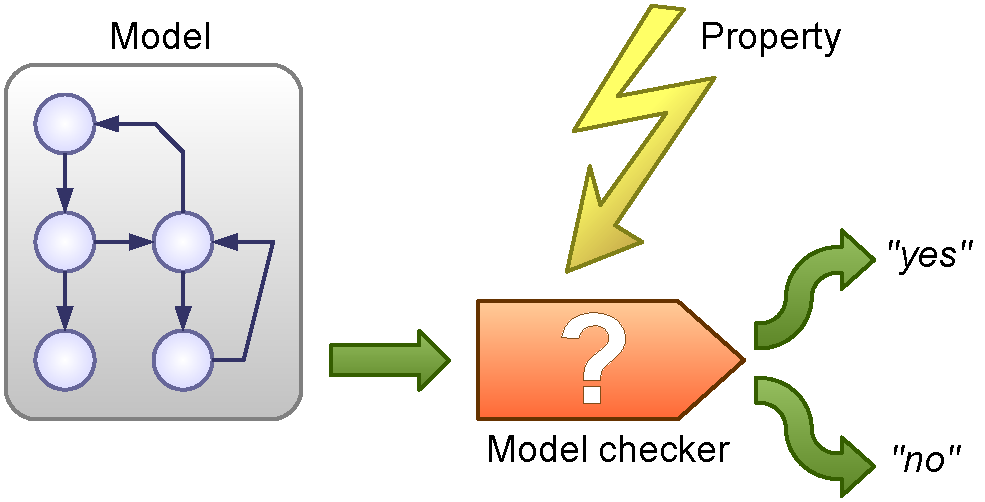
\includegraphics[width=0.9\textwidth]{content/timed-automata/model-checking}
    \caption{Principle of model checking.}
    \label{fig:model-checking}
\end{figure}

We briefly introduce the general principle of \emph{model checking} that we illustrated on Figure~\ref{fig:model-checking}. It refers to the process of testing \emph{properties} of a system for which a \emph{model} is given. The \emph{model checker} is a ``black box'' component that takes both of them as inputs then outputs whether the property is satisfied or not. Some model checkers can also output a \emph{trace}, mostly to give details of why the property cannot be satisfied (they are sometimes referred as \emph{error traces}).\\

The types of properties to be checked are usually classified in the following categories, although a model checker does not especially distinguish them. \emph{Reachability properties} check whether a property can possibly be satisfied by the system (e.g., \emph{``the light can be switched off''}). \emph{Safety properties} state that something which is considered as ``bad'' will never happen in the system (e.g., \emph{``the light cannot stay on for more than 20 minutes''}). Finally, \emph{liveness properties} state that something which is considered as ``good'' will eventually happen (e.g., \emph{``when the light is off, pressing the button turns it on''}).\\

Various timed automata model checkers have been proposed. They target different classes of timed automata as a model. They leverage timed temporal logics for expressing properties and query the models. We briefly present the main tools.\\

\begin{table}[htbp]
\footnotesize
\centering
\begin{tabular}{|p{4cm}|p{4cm}|p{4cm}|}

	\hline

	\textit{Tool} &
	\textit{Model} &
	\textit{Temporal logic} \\
	
	\hline
	
	Kronos \cite{KRONOS1,KRONOS2} &
	Timed automata &
	TCTL \\
	
	\hline
	
	HyTech \cite{HYTECH} &
	Hybrid automata \cite{ACHH93,alur97symbolic}  &
	ICTL, an extension of TCTL \cite{ACHH93} \\
	
	\hline
	
	UPPAAL \cite{UPPAAL} &
	Hybrid extension of timed automata &
	Subset of TCTL \\
	
	\hline
	
	Tempo \cite{MS01} &
	Event-recording timed automata &
	\emph{Event-recording fixpoint logic} defined in \cite{MS01} \\
	
	\hline

\end{tabular}
\label{tab:ta-model-checkers}
\caption{Model checking tools for classes and extensions of timed automata.}
\end{table}

\begin{figure}[htbp]
    \centering
    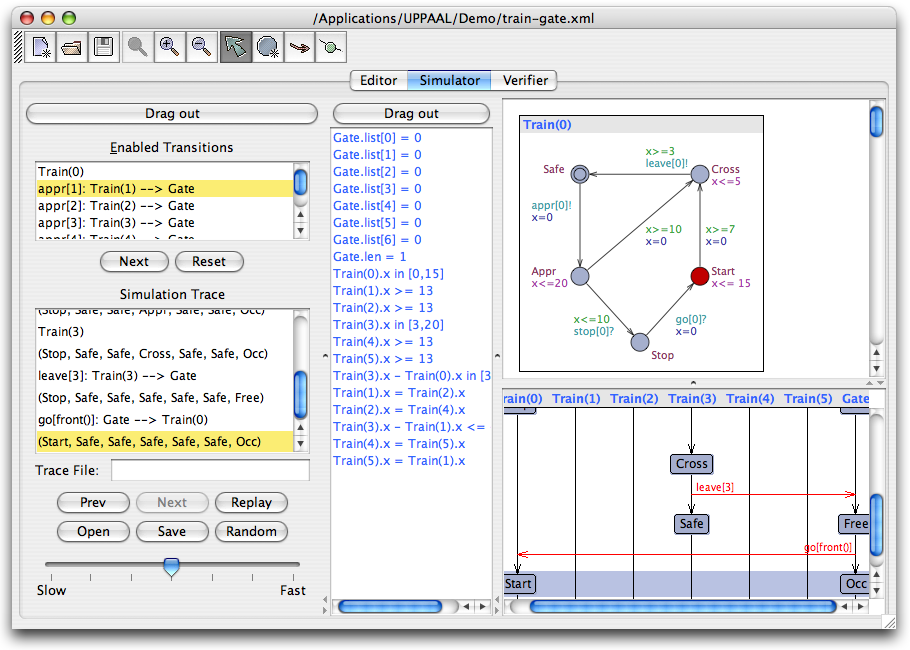
\includegraphics[width=\textwidth]{content/timed-automata/uppaal-2}
    \caption{A screenshot of UPPAAL.}
    \label{fig:uppaal}
\end{figure}

The tools are presented in Table~\ref{tab:ta-model-checkers}. Not surprisingly, branching timed temporal logics are popular given the decidability of the model checking problem. Tempo is specialized on event-recording timed automata and uses a logic developed on purpose. Kronos is the only tool to use ``canonical'' timed automata while UPPAAL and HyTech both use hybrid extensions. Briefly, an hybrid system \cite{alur97symbolic} features both continuous (e.g., variables in $\R$) and discrete behavior (e.g., variables in $\N$). At the time of the writing of this document, it should be noted that UPPAAL is the only actively developed project. UPPAAL has also managed to emerge from an academic research prototype to a commercial product for model checking. It has been used in several industrial studies (a complete list is available at \url{http://www.it.uu.se/research/group/darts/uppaal/examples.shtml}). We give a few references containing such case studies: \cite{HSLL97, HLS99, DAKRT97, LAAB98, dw00, lpw:tacas98, bowman98automatic, BGKLLPY96, lp:prfts97}.\\

A screenshot of the UPPAAL simulation environment is available on Figure~\ref{fig:uppaal}. A more detailed presentation of UPPAAL is available in the appendix from page~\pageref{chap:uppaal}.

% ........................................................................... %

% ........................................................................... %

% ........................................................................... %

\part{Protocol modeling and analysis}

% ........................................................................... %

\chapter{Timed protocol modeling}
\label{chap:timed-protocols}
% ........................................................................... %

This chapter presents the model of \emph{timed business protocols}. It is a formalization of the business protocol introduced in \cite{FTBB} and the timing constraints primitives that were mentioned in \cite{BBFC04,BCT-CAISE03}. By investigating (online) applications to define which type of timing abstraction would turn out to be useful in practice for describing the externally-observable behavior of services, we identified two primitives: \CInvoke constraints for defining time windows of availabilities and \MInvoke constraints for defining implicit actions that occur when some forms of delays expire. The introduction of timing constraints into the model poses significant challenges, especially when it comes to studying the impacts on protocol analysis as we will see in the next chapters. We obtained a characterization of timed protocols and their operators by establishing a link with the field of timed automata \cite{RADLD94}. This way, we will see that introducing timing constraints in business protocols is a significant challenge as it makes protocol analysis much more complex than in the untimed case. More specifically, we will see that with timed automata, complementation and subsumption are generally undecidable while \MInvoke constraints are hard to express. \\

The chapter is structured as follows. We first provide a concise discussion on the timing abstractions that we identified. Then, we present the model of timed business protocols that we envisioned as a conceptual model. Next, we explain how timed protocols can be equivalently expressed using \emph{timed automata} \cite{RADLD94}, a formal framework that has been extensively investigated in formal verification research works \cite{RAPM04,UPPAAL}. This will later allow us to derive theoretical properties for the model of timed protocols by establishing a semantic-preserving mapping between the two models. Finally, we provide a discussion.

% ........................................................................... %

\section{Timing abstractions}

% ........................................................................... %

Before designing our web services business protocols model, we started by investigating the timing abstractions that were needed to capture the ones that would be useful in practice. We first present three motivating examples, then introduce the two timing abstraction primitives that we have identified.

% ........................................................................... %

\subsection{Motivating examples}

Timing constraints appear in countless scenarios. We give here three examples related to web services and business processes were timing constraints play a critical role.

% ........................................................................... %

\subsubsection{E-Commerce portals}

The sales conditions notices of many E-Commerce portals provide timing constraints. Let us consider a classic example of a plane ticket seller portal. A potential purchaser is usually allowed to put a seat on hold for a day or two before a confirmation involving the effective payment is made. The seller implicitly releases the seat holding and cancels the purchase process after a delay (e.g., 24 hours) without a confirmation or canceling notification from the buyer. There are other examples in the field of E-Commerce examples. For example goods selling portals are usually entitled by law regulations to allow a buyer to return a purchase within a short delay such as one week after the delivery. They are often also constrained to respect delays when dealing with customers for operations such as the deliveries or the refunding of returned purchases.

\begin{figure}[htbp]
    \centering
    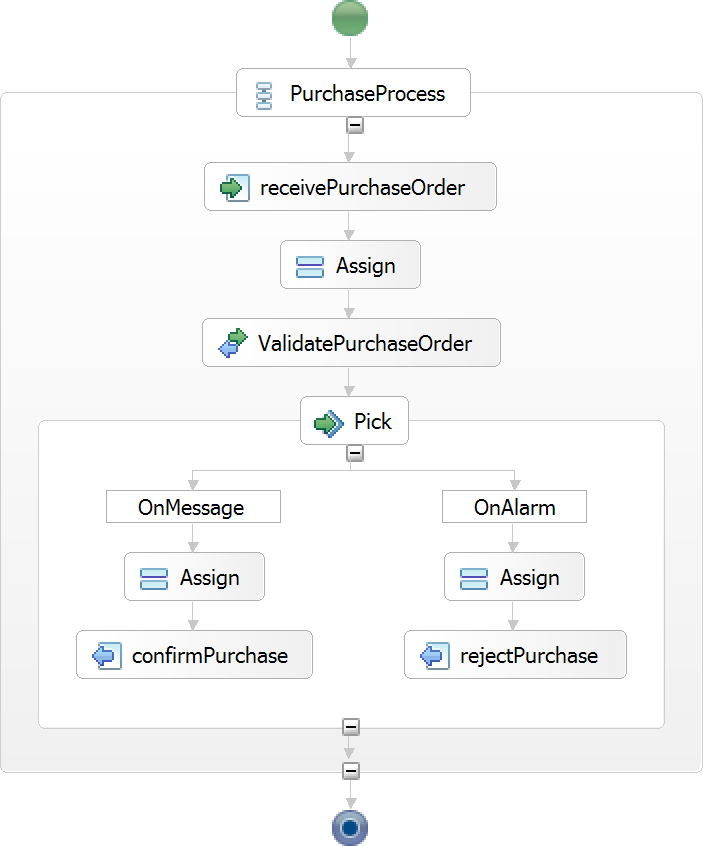
\includegraphics[height=11cm]{content/protocol-model/bpel-purchase}
    \caption{A BPEL process that uses an alarm.}
    \label{fig:bpel-purchase}
\end{figure}

\subsubsection{BPEL processes}

The \emph{Business Process Execution Language} \cite{WSBPEL2} is the major specification in the field of long-running web services orchestrations. A BPEL process is able to achieve a complex business process using a set of web services. Figure~\ref{fig:bpel-purchase} exhibits a sample purchasing BPEL process. The process starts by receiving a purchase order. A BPEL \emph{Assign} operation is then executed to prepare the data for the invocation of a service providing a \emph{ValidatePurchaseOrder} operation. This operation is used to delegate the processing of the purchase order to a service that will check for various conditions like the ordered items availability, the existence of contracts between the requesting entity and the provider, the validity of the chosen payment option and checking that the requesting entity does not have outstanding debts to the provider. Given that those checkings may take a substantial amount of time (for examples humans have to be involved for some of the checkings), the process uses a \emph{pick} block. It allows to wait for receiving a response that validates the order. If no response has been received after an arbitrary delay such as 48 hours, the process is woken-up to reject the purchase. BPEL actually exhibits two similar time-related constructs: \emph{onAlarm} and \emph{wait}. The former can be used in \emph{pick} blocks, while the later is a normal BPEL operation that will put the process execution on hold for a duration or until a fixed date is reached.

\begin{figure}[htbp]
    \centering
    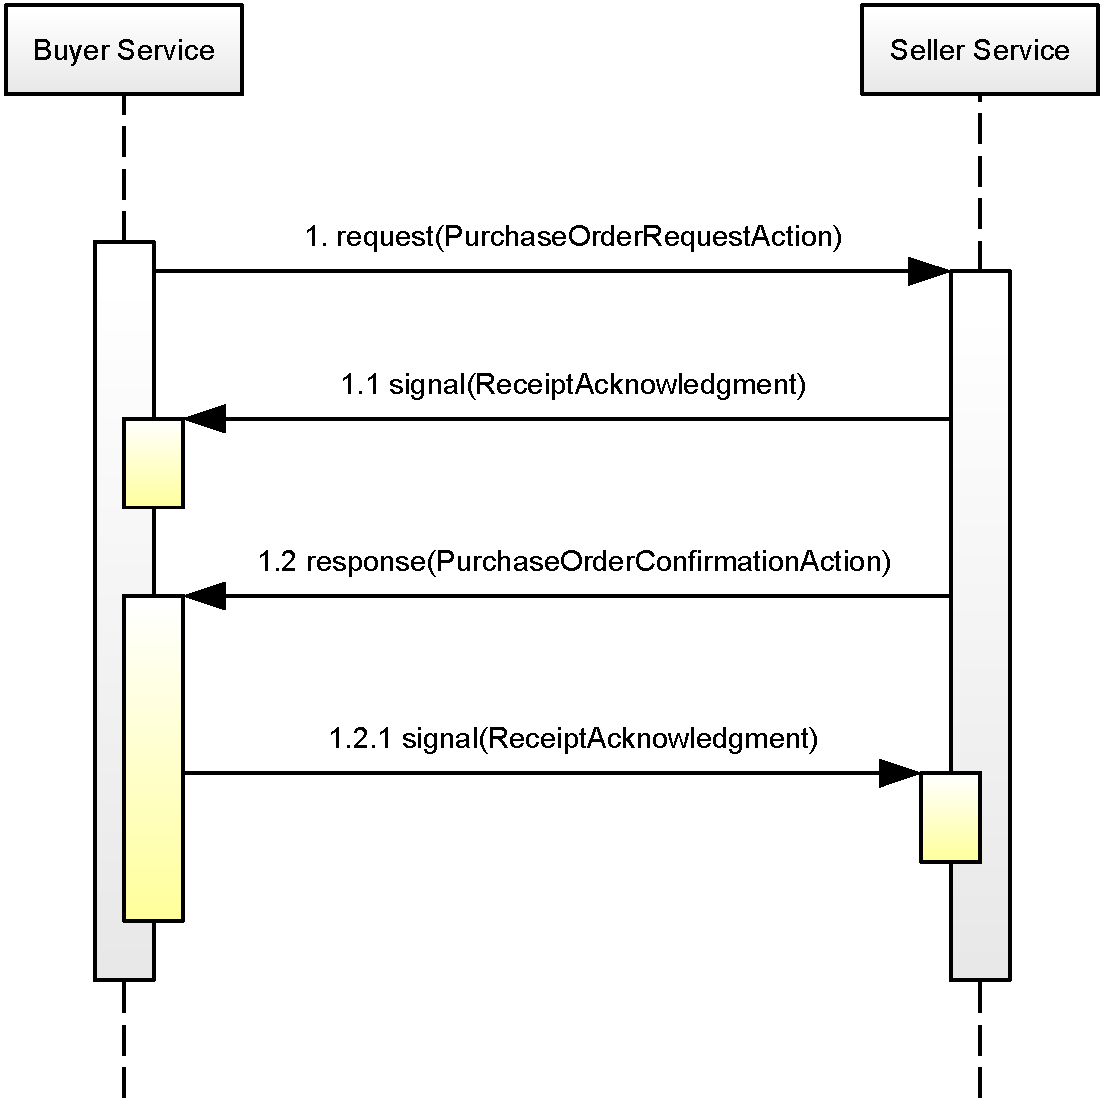
\includegraphics[width=\textwidth]{content/protocol-model/pip3a4}
    \caption{Sequence diagram of the RosettaNet PIP 3A4 (Request Purchase Order).}
    \label{fig:pip3a4}
\end{figure}

\subsubsection{RosettaNet PIPs}

RosettaNet \cite{ROSETTANET} is an industrial consortium which aims at facilitating the transactions among the supply chains of trading partners using specifications called the \emph{Partner Interface Processes} (PIPs) that thoroughly detail the processes involved in those transactions. The RosettaNet PIPs exhibit time-dependent behaviors. Let us focus on the PIP 3A4 depicted on Figure~\ref{fig:pip3a4}. It specifies how a seller and a buyer can process a purchase order. This PIP specifies the following timing constraints:
\begin{itemize}

    \item the \emph{PurchaseOrderRequestAction} and the \emph{PurchaseOrderConfirmationAction} must be acknowledged within 2 hours

    \item the reply to the \emph{PurchaseOrderRequestAction} must be sent within 24 hours.

\end{itemize}

% ........................................................................... %

\subsection{Timing abstraction primitives}

% ........................................................................... %

The three motivating examples that we gave illustrate the need for capturing timing abstractions into web services and business process models. We did not limit our investigations to these examples in order to identify the primitives that would be useful to capture the vast majority of cases appearing in practice. A major difficulty when designing a model is to find a good expressiveness level tradeoff. Indeed, a simplistic model does not capture all of the cases while an overly complex one becomes hard to use for practitioners, and may lead to undecidability problems in algorithms.\\

The starting point of this work was done in \cite{BCT-CAISE03,KBBB+04}. Using a similar approach based on the exploration of existing web portals and E-Commerce websites, we found that the following timing primitives would be useful.

\paragraph{Time windows.} Many actions need to be available only during certain time windows. For example, a quotation usually has a finite validity, and a purchase cannot be made in the same conditions once it has expired. Another example in the commerce domain is the case of discounts which can be valid only for a limited period of time.

\paragraph{Timeouts.} Most software systems support the notion of timeout, for example to avoid locking resources for an unlimited amount of time and to handle partnering components errors. Considering again an example in the commerce domain, a purchase order needs to be paid to be validated. A seller system will usually discard the business transaction after a given delay if the buyer did not actually send the payment.

% ........................................................................... %

\section{Extending business protocols with temporal abstractions}

% ........................................................................... %

We now present the \emph{timed business protocol} model. We first illustrate it informally, then provide a formalized definition.

% ........................................................................... %


\subsection{Timed business protocols}

% ........................................................................... %

Our model is an extension of the \emph{business protocol} model \cite{BBFC04,FTBB} which is built upon the traditional state-machine formalism. Indeed, it is commonly used to model the behavior of systems, due to the fact that it is simple and intuitive.
In the model, states represent the different phases that a service may go through during its interaction with a requester. A transition label is a message supported by the service. It has a polarity which is positive ($+$) if the message is incoming, or negative $(-)$ if it is outgoing. Transitions are triggered when their associated messages are sent or received. Hence, a state identifies a set of outgoing transitions, and therefore a set of possible messages that can be either sent or received when the conversation with a requester is in this state.\\

\begin{figure}[thbp]
    \centering
    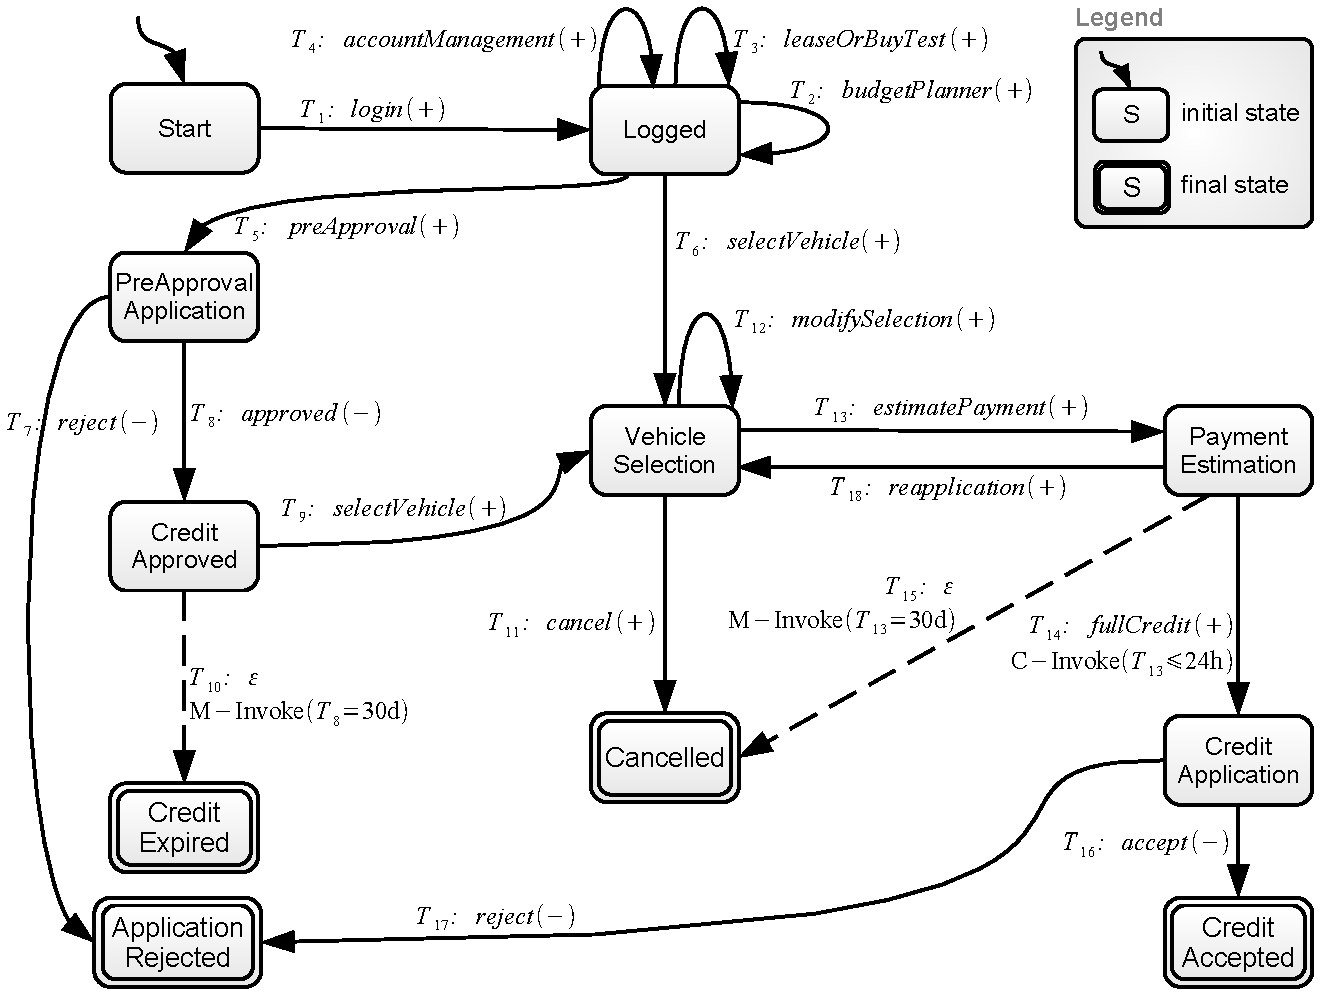
\includegraphics[width=\textwidth]{content/protocol-model/ford-credit}
    \caption{A timed protocol of an online financing service.}
    \label{fig:ford-credit}
\end{figure}

As an example, the protocol depicted on Figure~\ref{fig:ford-credit} (inspired by the \emph{Ford Credit web portal}) is initially in the $Start$ state, and requesters begin a conversation by sending a $login$ message, moving to the $Logged$ state.\\

In the figure, the initial state is indicated by an unlabeled entering arrow while final states are double-circled. A conversation is accepted when ending in such a final state. Hence, a sequence of messages $login(+) \cdot preApproval(+) \cdot reject(-)$ is a conversation supported by the protocol, while $selectVehicle(+) \cdot login(+)$ is not: no transition for a $selectVehicle$ message is available from the $Start$ state, the two messages cannot be ordered this way, and the conversation does not end in a final state.  Business protocols must be deterministic, as the requesters always need to be able to determine in which state the service is, else much of the purpose of the protocol specification would be lost.\\

We consider the following two extensions to the base protocol model:
\begin{enumerate}

    \item \CInvoke constraints specify time windows within which a transition \emph{can} be fired. Outside of those time windows, the transition is disabled, and exchanging the associated message results in an error.
    
    \item \MInvoke constraints specify \emph{when} a transition is \emph{automatically} fired.
    
\end{enumerate}

The obtained model  is called  \emph{timed (business) protocol model}.
\CInvoke constraints can be attached to \emph{explicit} transitions for which a message is exchanged between the service provider and its requesters. The absence of \CInvoke constraint on an explicit transition means that it can be fired from its source state at any time.
By contrast, \MInvoke constraints are associated to \emph{implicit} transitions. They model state changes in conversations once a delay has elapsed (a typical example being a timeout). They are not related to message exchanges between the service provider and its requesters. Implicit transitions are analogous to the silent transitions in the automata theory \cite{Hopcroft79} and we associate the empty word $\varepsilon$ as the label of those transitions. There is however a significant difference compared to ``classical'' automata: they cannot be removed in the general case as we will see later. \\

Continuing with the example protocol depicted on Figure~\ref{fig:ford-credit}, it is indicated that a full credit application is accepted only if it is received at most 24 hours after a payment estimation has been made. This behavior is specified by tagging the transition $T_{14}: fullCredit(+)$ with a time constraint $\CInvoke(T_{13} \leq 24h)$, i.e., $T_{14}$ can only be fired within a time window $[0h, 24h]$ after $T_{13}$ has been fired. $T_{10}$ has a constraint $\MInvoke(T_8 = 30d)$, meaning that once a pre-approval application has been approved ($T_8$), a requester is given 30 days to select a vehicle ($T_9$). If it does not continue the conversation by sending a $selectVehicle$ message within the next 30 days, then the service provider will automatically fire $T_{10}$ and move to the $CreditExpired$ state, ending the conversation. Finally, it should be noted that the presence of an implicit transition from a given state affects the time constraints of the explicit transitions outgoing from the same state. Indeed, $T_{10}$ implies that $T_9$ can only be fired within a time window matching the 30 days. Hence, a constraint $\CInvoke(T_8 < 30d)$ is implicitly associated with $T_9$ because of the \MInvoke constraint of $T_{10}$.\\

\begin{figure}[htbp]
    \centering
    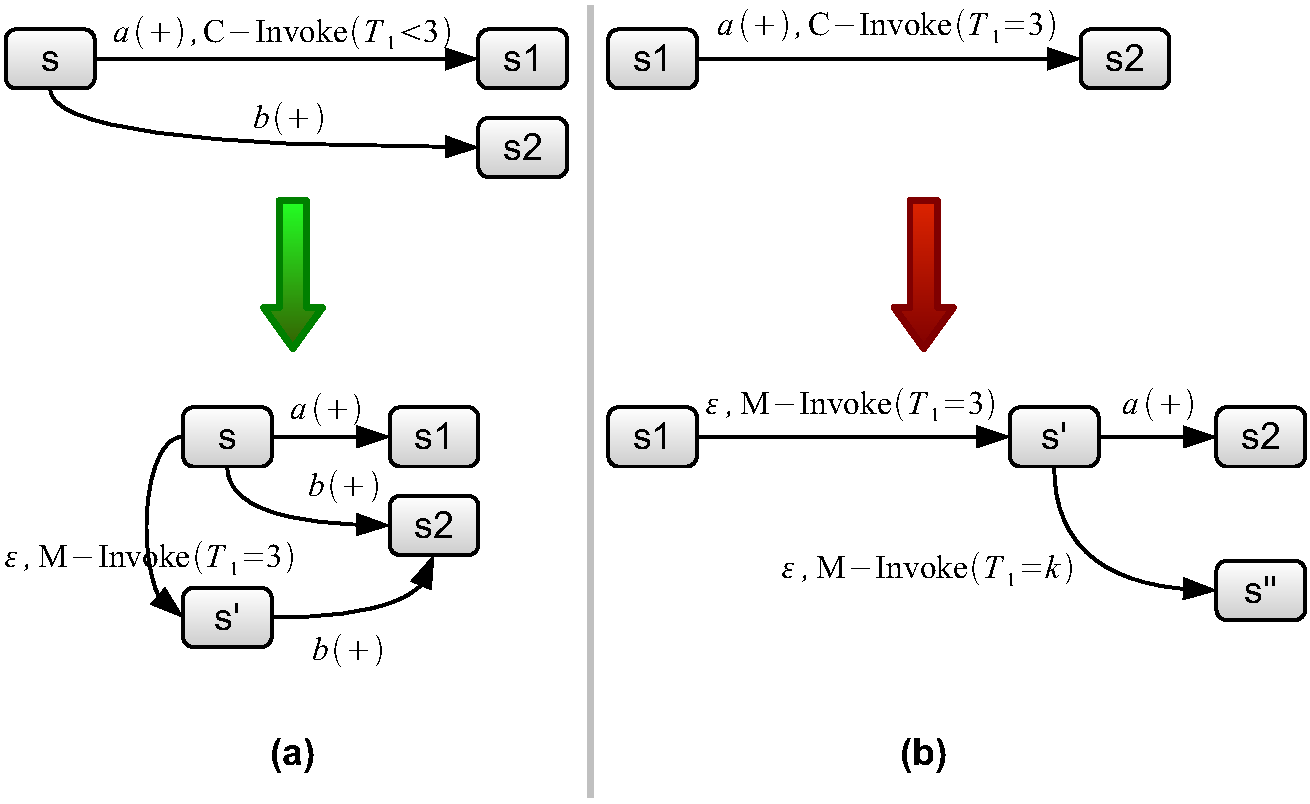
\includegraphics[width=\textwidth]{content/protocol-model/ci-vs-mi}
    \caption{Examples for illustrating why both \CInvoke and \MInvoke are necessary.}
    \label{fig:ci-vs-mi}
\end{figure}

Both \CInvoke and \MInvoke constraints are orthogonal. Indeed, we will see in Theorem~\ref{thm:mi-expressiveness} that the transitions having \MInvoke constraints strictly increase expressiveness of our model. Naturally, the usefulness of \CInvoke constraints can be questioned as in many cases, a \CInvoke-free construction can be made by using extra states and \MInvoke constraints on implicit transitions. Let us consider the examples of Figure~\ref{fig:ci-vs-mi}. The case (a) is simple as the \CInvoke constraint is easily translated using \MInvoke by adding an extra state $s'$.
This is however not true in the general case as the (b) counter example shows as it yields the following problem: $k \in \Q$ cannot be determined as the set of rational numbers is infinite, hence we cannot find a value for $k$ that would be ``close-enough'' to $3$ for ensuring that $a(+)$ is only received when $T_1$ is exactly equal to $3$.

% ........................................................................... %

\subsection{Formalization}

% ........................................................................... %

\subsubsection{Syntax}

% ........................................................................... %

Before giving the definition of timed protocols, we need to formalize the \CInvoke and \MInvoke constraints.
Let $\mathcal{X}$ be a set of variables referring to transition identifiers: if $r$ is a transition then $T_r \in {\mathcal{X}}$ is the variable referring to this transition. We consider the two kinds of time constraints defined over a set of variables $\mathcal{X}$ using the following grammars:
\begin{itemize}

    \item $\CInvoke{(c)}$ with  $c$ defined as follows:
    $$ c ::= x \; op \; k \; | \; x - x' \; op \; k \; | \; c \wedge c \; | \; c \vee c $$
    with  $op \in \{=, \neq, <, >, \leq, \geq\}$,
     $x \in \mathcal{X}$, $x' \in \mathcal{X}$ and $k \in \Q \cup \{ \perp \}$, where $\Q$ denotes the set of positive rational numbers,

    \item $\MInvoke{(c)}$ with $c$ defined as follows:
    $$ c ::= (x = k) \wedge c' \; | \; c \wedge c \; | \; c \vee c $$
    with $x \in \mathcal{X}$, $k \in \Q \cup \{ \perp \}$ and $c'$ being defined like in the grammar of \CInvoke constraints.

\end{itemize}

The following is the definition for timed business protocols, extending the business protocols model \cite{BBFC04,FTBB}.

\begin{definition}
A \emph{timed business protocol} is a tuple $\mathcal{P} = (\mathcal{S}, s_0, \mathcal{F}, \mathtt{M}, \mathcal{X}, \mathcal{C}, \mathcal{R})$ where:
\begin{itemize}

  \item $\mathcal{S}$ is a finite set of states, with $s_0 \in \mathcal{S}$ being the initial state.

  \item $\mathcal{F} \subseteq \mathcal{S}$ is the set of final states. If $\mathcal{F} = \emptyset$, then $\mathcal{P}$ is said to be an empty protocol.

  \item $\mathtt{M} = \mathtt{M_e} \cup \{\varepsilon\}$ is a finite set of messages $\mathtt{M_e}$ augmented with the empty message $\varepsilon$. For each message $m \in \mathtt{M_e}$, we define a function $\polarity{\mathcal{P}}{m}$ which will be positive $(+)$ if $m$ is an input message in $\mathcal{P}$, and negative $(-)$ if $m$ is an output message in $\mathcal{P}$.

  \item We assume that each transition $r \in \mathcal{R}$ is identified by a unique identifier $id(r)$. $\mathcal{X} = \{ T_i \;|\; \exists r \in \mathcal{R},\; T_i = id(r) \}$ is a set of clock variables defined over the set of transitions $\mathcal{R}$.

  \item $\mathcal{C}$ is a set of time constraints defined over a set of variables $\mathcal{X}$. The absence of a constraint is interpreted as a constraint which always evaluates to $\mathtt{true}$.

  \item $\mathcal{R} \subseteq \mathcal{S}^2 \times \mathtt{M} \times \mathcal{C}$ is a finite set of transitions.
  Each transition $(s, s', m, c)$ identifies a source state $s$, a target state $s'$, a message $m$ and a constraint $c$. We say that the message $m$ is enabled from a state $s$. When $m = \varepsilon$, $c$ must be a \MInvoke constraint,  otherwise $c$ must be either a \CInvoke constraint or $\mathtt{true}$.

\end{itemize}
\end{definition}

In the sequel, we use the notation $\mathcal{R}(s, s', m, c)$ to denote the fact that $(s, s', m, c) \in \mathcal{R}$. To enforce determinism, we require that a protocol has only one initial state, and  that for every state $s$ and every two transitions $(s, s_1, m_1, c_1)$ and $(s, s_2, m_2, c_2)$ enabled from $s$, we have either $m_1 \neq m_2$ or $c_1 \wedge c_2 \equiv \mathtt{false}$.

% ........................................................................... %

\subsubsection{Semantics}

% ........................................................................... %

\paragraph{Variable interpretation.}
Defining the timed protocol semantics requires the introduction of the notion of variable valuation. We consider as a time domain the set of positive reals $\Rpos$ augmented with a special element $\perp$ to denote the fact that a transition has never been taken yet.
Let $\mathcal{X}$ be a set of variables valued in $\Rpos$. A variable valuation
$$ \val : {\mathcal{X}} \rightarrow \Rpos \cup \{ \perp \} $$
is a mapping that assigns to each variable $x \in {\mathcal{X}}$ a time value $\val(x)$.\\

We note by $\val_{t}(x)$ the valuation of $x$ at an instant $t$. In the beginning (i.e., at instant $t_0 = 0$) we assume that all of the variables are set to $\perp$, i.e., $\val_{{t_0}}(T_i) = \perp, \forall T_i \in {\mathcal{X}}$.\\

Then, a variable valuation at a time $t_j$ is completely determined by a protocol execution. Consider for example an execution $\sigma = s_0 \cdot (m_0, t_0) \cdot s_1 \ldots s_{n-1}.(m_{n-1}, t_{n-1}) \cdot s_n$ of a protocol $\mathcal{P}$. The valuation of a clock variable $T_i$ at time $t_j$, with $0 < j \leq n$, is defined as follows:
$$
\val_{{t_j}}(T_i) =
\left \{
  \begin{array}{l}
  
    \val_{t_{j-1}}(T_i) + (t_j - t_{j-1}) \\
    
    0 \mbox{ if } T_i = id(\mathcal{R}(s_j, s_{j+1}, m, c)) \mbox{ is fired from  } s_j \mbox{ to } s_{j+1} \\
  
  \end{array}
\right.
$$
It should be noted that for any $r \in \Rpos$, $k \in \Q$ and any comparison operator $op \in \{<, \leq, =, \neq, >, \geq \}$:
$$
\left\lbrace
\begin{array}{l}
  \perp +\; r =\; \perp \\
  \perp -\; r =\; \perp \\
  \perp op\; k = \mathtt{false} \\
  \perp op \perp \; = \mathtt{true} \mbox{ if } op \in \{ =, \leq, \geq \} \\
  \perp op \perp \; = \mathtt{false} \mbox{ otherwise }\\
\end{array}
\right.
$$

Given a variable valuation $\val$ and a constraint $\CInvoke{(c)}$ (respectively, $\MInvoke{(c)}$), we note by $c(\val)$, the constraint obtained by substituting each variable $x$ in $c$ by its value $\val(x)$. A variable valuation $\val$ satisfies a constraint $\CInvoke{(c)}$ (respectively, $\MInvoke{(c)}$) if and only if
$c(\val) \equiv \mathtt{true}$. In this case, we write $\val\ \models \CInvoke{(c)}$ (respectively, $\val \models \MInvoke{(c)}$)

\paragraph{Timed conversations.}
Timed conversations are inspired from the notion of \emph{timed words} in timed automata as defined in \cite{RADLD94}.\\

Let $\mathcal{P} = (\mathcal{S}, s_0, \mathcal{F}, \mathtt{M}, \mathcal{X}, \mathcal{C}, \mathcal{R})$ be a timed protocol. A \emph{correct execution} (or simply, an execution) of $\mathcal{P}$ is a sequence $\sigma = s_0 \cdot (m_0, t_0) \cdot s_1 \ldots s_{n-1} \cdot (m_{n-1}, t_{n-1}) \cdot s_n$  such that:
\begin{enumerate}

    \item $t_0 \leq t_1 \leq \ldots \leq t_n$ (i.e., the occurrence of times increase monotonically),

    \item $s_0$ is the initial state and $s_n$ is a final state of $\mathcal{P}$, and

    \item $\forall j \in [1,n]$, we have: $\mathcal{R}(s_{j-1}, s_{j}, m_{j-1}, c_{j-1})$ and $\val_{j-1} \models c_{j-1}$.
\end{enumerate}

\begin{sloppypar}
As an example, the sequence
$\sigma' = Start \cdot (login(+), 0) \cdot Logged \cdot (preApproval(+), 1) \cdot PreApprovalApplication
\cdot (approved(-), 3) \cdot CreditApproved \cdot (\varepsilon, 33) \cdot CreditExpired$
is a correct execution of the financing service protocol depicted on Figure~\ref{fig:ford-credit}.
\end{sloppypar}\

If $\sigma = s_0 \cdot (m_0, t_0) \cdot s_1 \ldots s_{n-1} \cdot (m_{n-1}, t_{n-1}) \cdot s_n$ is a correct execution of $\mathcal{P}$, then the sequence $tr(\sigma) = (m_0, t_0) \ldots (m_{n-1}, t_{n-1})$ forms a \emph{timed trace} which is compliant with  $\mathcal{P}$.
Continuing with the example, the execution $\sigma'$ of the above service protocol leads to the timed trace $tr(\sigma') = (login(+), 0) \cdot (preApproval(+), 1) \cdot (approved(-), 3) \cdot (\varepsilon, 33)$.\\

During an execution $\sigma$ of a protocol $\mathcal{P}$, the externally observable behavior of $\mathcal{P}$, hereafter called \emph{timed conversation} of $\mathcal{P}$ and noted $conv(\sigma)$, is obtained by removing from the corresponding timed trace $tr(\sigma)$ all of the non observable events (i.e., all of the pairs $(m_i, t_i)$ with $m_i = \varepsilon$). For example, during the previous execution $\sigma'$, the observable behavior of the financing service is described by the timed conversation $obs(\sigma') = (login(+), 0) \cdot (preApproval(+), 1) \cdot (approved(-), 3)$.\\

In the following, given a protocol $\mathcal{P}$, we denote by $Tr(\mathcal{P})$  the set of timed conversations of $\mathcal{P}$.

\paragraph{Timed interactions.}
Timed conversations describe the externally observable behavior of timed protocols and, as we will show below, are essential to analyze the ability of two services to interact correctly.
Consider for example the protocol $\mathcal{P}$ depicted on Figure~\ref{fig:ford-credit} and its reversed protocol $\mathcal{P'}$ obtained by reversing the polarity of the messages (i.e., input messages become outputs and vice-versa).

\begin{sloppypar}
We can observe that when $\mathcal{P'}$  interacts with $\mathcal{P}$ by following a given timed conversation, $\mathcal{P}$ follows exactly a conversation with the reversed polarities of the messages. For example, if during such an interaction the timed conversation of $\mathcal{P}$ is $(login(+), 0) \cdot (selectVehicle(+), 1) \cdot (estimatePayment(+), 10) \cdot (fullCredit(+), 30) \cdot (accept(-), 100)$, then the timed conversation of $\mathcal{P'}$ is $(login(-), 0) \cdot (selectVehicle(-), 1) \cdot (estimate\-Payment(-), 10) \cdot (fullCredit(-), 30) \cdot (accept(+), 100)$.
\end{sloppypar}\

\begin{sloppypar}
In this case, we call the path $(login, 0) \cdot (selectVehicle, 1) \cdot (estimatePayment, 10) \cdot (fullCredit, 30) \cdot (accept, 100)$ a \emph{timed interaction trace} of $\mathcal{P}$ and $\mathcal{P'}$. The polarities of the messages that appear in interaction traces are not defined. Indeed, each input message $m$ of one protocol matches an output message $m$ of the other protocol.
\end{sloppypar}\

More precisely, let $\mathcal{P}$ and $\mathcal{P}'$ be two timed protocols and let $\tau = (a_0, t_0) \cdot (\ldots) \cdot (a_n, t_n)$ be a sequence of events in which the polarities of the messages are undefined. Then $\tau$ is a timed interaction trace of $\mathcal{P}$ and $\mathcal{P}'$ if and only if there exist two timed conversations $\sigma_1$ and $\sigma_2$ such that:
\begin{enumerate}

    \item $\sigma_1 \in Tr(\mathcal{P})$ and  $\sigma_2 \in Tr(\mathcal{P}')$, and

    \item $\sigma_1$ is the reverse conversation of $\sigma_2$ (i.e., the conversation obtained from $\sigma_2$ by inverting the polarities of the messages), and

    \item $\tau = Unp(\sigma_1) = Unp(\sigma_2)$ where $Unp(\sigma)$ denotes the trace obtained from $\sigma$ by removing the polarities of the messages.

\end{enumerate}

% ........................................................................... %

\section{From timed protocols to protocol timed automata}

% ........................................................................... %

The previous section has introduced the model of timed business protocols which is suitable for describing the external behavior of web services, including timing constraints. In turn, the model of timed automata \cite{RADLD94} has been extensively studied as an extension of classical automata \cite{Hopcroft79} with real-valued clocks and conditions on the transitions. Given the extensive research that has been made on timed automata, we chose to:
\begin{enumerate}
  
  \item use timed protocols as a conceptual model, and
  
  \item use timed automata for implementing the behavior of timed protocols, and
  
  \item derive theoretical properties of timed protocols from existing work on timed automata.
  
\end{enumerate}
To do that, we give a mapping from timed protocols to a new class of timed automata that we identified, called \emph{protocol timed automata}. However, defining such a mapping is not a trivial task as we will see that \MInvoke constraints are not straightforward to implement using timed automata.\\  

This section is structured as follows. We start by an informal, illustrated walk through the challenges of converting a timed protocol to a timed automaton that correctly implements its behavior. We then briefly define the class of protocol timed automata. Then, we formally study the \MInvoke constraints enforcement techniques for timed automata.

% ........................................................................... %

\subsection{Informal overview of the challenges}

% ........................................................................... %

\begin{figure}[htbp]
    \centering
    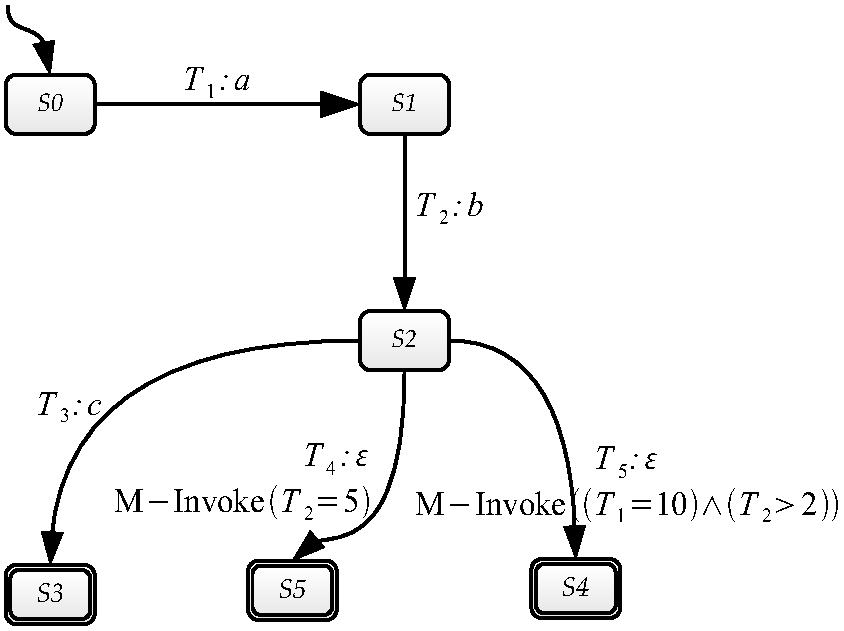
\includegraphics[width=\textwidth]{content/protocol-model/pta-protocol}
    \caption{A sample timed protocol $\mathcal{P}$ used as a mapping running example.}
    \label{fig:pta-protocol}
\end{figure}

We will use the timed protocol from Figure~\ref{fig:pta-protocol} as a running example throughout this section. It will allow us to illustrate the challenges in creating a timed automaton that behaves like a timed protocol. At first sight, the translation may look straightforward. However as we will see, preserving the behavior of \MInvoke is surprisingly not an easy task. The translation is performed using a mapping that we now illustrate. The mapping is done in two steps.\\

The first step to convert a timed protocol $\mathcal{P}$ into a timed automaton $A$ is relatively simple. The mapping of the states of $\mathcal{P}$ to the locations of $A$ is direct (e.g., the state $s_0$ of $\mathcal{P}$ is mapped to a location $l_0$). Similarly, each transition in $\mathcal{P}$ is translated as a switch with the message name as its label (e.g., in $\mathcal{P}$, $T_1: \mathcal{R}(s_0, s_1, a, \mathtt{true})$ is translated as a switch $e_1 = (l_0, \mathtt{true}, a, r, l_1)$ in $A$). Also, the initial location and the final locations in $A$ correspond to the initial and final states in $\mathcal{P}$.\\

\begin{figure}[htbp]
    \centering
    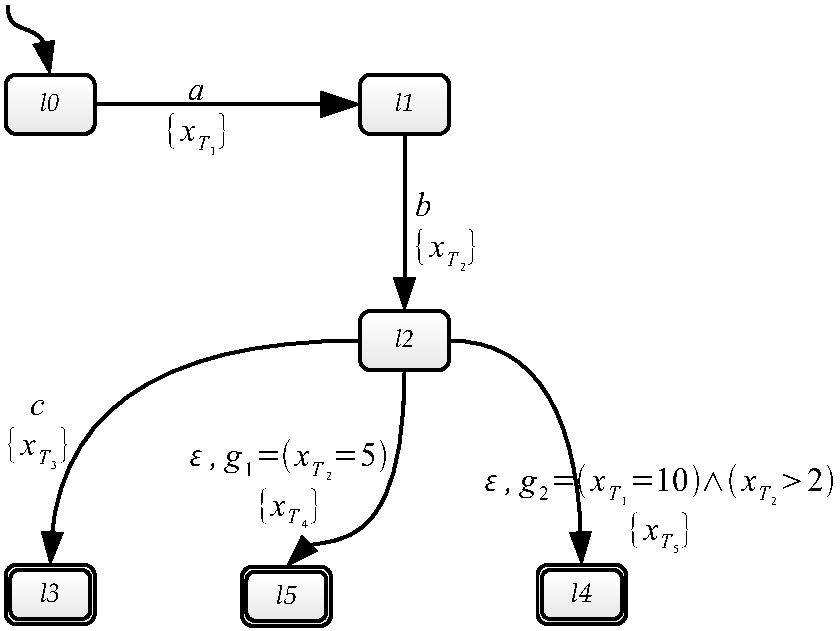
\includegraphics[width=\textwidth]{content/protocol-model/bogus-pta-constraint}
    \caption{A sample timed automaton that does not enforce M-Invoke semantics.}
    \label{fig:bogus-pta-constraint}
\end{figure}

The transition identifiers from $\mathcal{P}$ are used to generate clocks in $A$. Indeed, each identifier generates a unique clock which is solely reset on its corresponding switch. For example the transition $T_2$ generates a clock $x_{T_2}$ in $A$ which is only reset on the switch that was mapped from $T_2$. This way, we can know when a switch was fired, just like in the timed protocol $\mathcal{P}$. The conversion of a \CInvoke constraint from $\mathcal{P}$ is also direct. For example, a constraint $\CInvoke(T_1 < 3)$ is mapped to a guard $(x_{T_1} < 3)$. At this stage, the mapping of $\mathcal{P}$ to $A$ yields the timed automaton of Figure~\ref{fig:bogus-pta-constraint}.\\

Assuming that we mapped implicit transitions as $\varepsilon$-labeled switches with a direct translation of \MInvoke constraints into guards, the following problems arise on the timed automaton of Figure~\ref{fig:bogus-pta-constraint} when the current location is $l_2$.
\begin{enumerate}

	\item \textbf{Indeterminism:} $g_1$ and $g_2$ from Figure~\ref{fig:bogus-pta-constraint} can potentially become satisfied at the same time, and the $c$-labeled transition can be taken at the same time as either $g_1$ or $g_2$ is satisfied.
	
	\item \textbf{Semantics of \MInvoke constraints:} if one of the labeled switch guard $g_1$ or $g_2$ Figure~\ref{fig:bogus-pta-constraint} becomes satisfied while in $l_2$, it is not necessarily taken. Worse, the $c$-labeled switch can still be activated afterward.

\end{enumerate}
As a consequence, the timed automaton of Figure~\ref{fig:bogus-pta-constraint} does not respect the semantics of \MInvoke constraints, and they require more investigations to both enforce that $\varepsilon$-labeled switches are taken when their guards are satisfied, and that the other switches become ``disabled'' as soon as those guards become satisfied. As we will see, indeterminism is relatively easy to solve. However, ensuring that the semantics of \MInvoke constraints are enforced is a more involved task.\\

Let us have closer look at the various cases when entering a location that offers one $\varepsilon$-labeled switch. We illustrate that again on the location $l_2$ and the guard $g_2$ of Figure~\ref{fig:bogus-pta-constraint}.
Three cases are possible. The first one is that $l_2$ is entered before $g_2$ has been satisfied (i.e., $(x_{T_1} < 10)$ is true). In this case $c$ can be recognized as long as $(x_{T_1} < 10)$. The second case is that $l_2$ is entered when the valuation of $x_{T_1}$ is such that $(x_{T_1} > 10)$: $c$ can be recognized at any time since $g_2$ is not going to be satisfied for any successive clocks valuation. Finally, if $l_2$ is entered while $(x_{T_1} < 10)$, for any clocks valuation such that $(x_{T_1} \geq 10)$, $c$ can be recognized if and only if when $(x_{T_1} = 10)$ was true, $(x_{T_2} > 2)$ was false. The generalization to more than one constraint is similar, and will be detailed later. \\

Clearly, a direct translation of the constraints to guards is not enough to properly represent \MInvoke constructions in timed automata. Because of that, more elaborated constraints need to be added into the guards than a direct translation does. More specifically:
\begin{enumerate}

	\item the mapping needs to rewrite some guards to enforce the expected behavior of \MInvoke constraints, and 
	
	\item there is a need for knowing the exact clock valuations when a location is entered:
	\begin{enumerate}
	
		\item to know the status of each equality clause in each $\varepsilon$-labeled switches (e.g., when $l_2$ is entered, do we have $(x_{T_2} < 5)$? $(x_{T_2} > 5)$?)
		
		\item to know if the $\varepsilon$-labeled switches guards will be satisfiable or not (e.g., $g_2$) when their equality clause is satisfied.
	
	\end{enumerate}

\end{enumerate}
Especially, knowing the valuation of each clock when a location was entered is important for enabling / disabling some switches. For example when entering $l_2$, if $x_{T_2}$ was already greater than $5$, then there is no way the $\varepsilon$-labeled switch whose guard is $g_1$ can be enabled, and thus it should not disable the $c$-labeled switch nor the other $\varepsilon$-labeled switch. \\

In timed automata, the difference between 2 clocks $x_1$ and $x_2$ is a constant until either of them is reset as clocks evolve synchronously. Guards allow \emph{diagonal constraints}, i.e., constraints of the form $(x_1 - x_2 \;\#\; k)$ in the guards ($x_1, x_2$ being clocks and $k \in \Q \cup{ \perp }$). We use such diagonal constraints to capture the the clock valuations when locations are entered: for each location offering at least one $\varepsilon$-labeled switch, we add a clock that is attached to this location. Such a clock is reset on every incoming switch of the considered location. For example on Figure~\ref{fig:bogus-pta-constraint}, we add a clock $y_{l_2}$ which is reset on the $b$-labeled switch. Then, the difference between any clock $x_e$ and such a ``location clock'' $y_l$ is the exact value of $x_e$ when the location $l$ was entered. Indeed, when the location is entered, the valuation of $y_l$ is 0 as the clock has just been reset. Given that the difference between the two clocks remains a constant while $l$ remains the current location, $(x_e - y_l)$ is the clocks valuation of $x_e$ when $l$ was entered.\\

Using this technique to capture the clock valuations when a location is entered, the second step of the mapping can be done by rewriting the guards of every switch whose source location offers $\varepsilon$-labeled switches. The rewriting must take care of allowing normal (i.e., non $\varepsilon$-labeled switches) to recognize input symbols when \MInvoke constraints allow it, and block them otherwise. As we will see later in this chapter, we will introduce a clocks constraint function to capture \emph{when} a given switch is allowed with respect to the guard of a $\varepsilon$-labeled switch.\\

Going back to the example of Figure~\ref{fig:bogus-pta-constraint} with a new clock $y_{l_2}$ having been added, observe that $g_1$ must enable the other switches in the following two cases:
\begin{enumerate}
  
  \item $(x_{T_2} < 5)$, and
  
  \item $(x_{T_2} > 5) \wedge (x_{T_2} - y_{l_2} > 5)$
  
\end{enumerate}
While the first case is rather easy (i.e., $l_2$ is entered before the equality clause has been satisfied), the second case uses the valuation of $x_{T_2}$ when $l_2$ was entered. $(x_{T_2} - y_{l_2} > 5)$ is only true if $l_2$ was entered when $(x_{T_2} > 5)$ was true.\\

In a similar manner, $g_2$ enables the other switches in the following cases:
\begin{enumerate}
  
  \item $(x_{T_1} < 10)$, and
  
  \item $(x_{T_1} > 10) \wedge (x_{T_1} - y_{l_2} > 10)$, and

  \item $(x_{T_1} > 10) \wedge (x_{T_1} - y_{l_2} \leq 10) \wedge (x_{T_2} - x_{T_1} \leq -8)$, and
  
  \item $(x_{T_1} = 10) \wedge (x_{T_2} - x_{T_1} \leq -8)$
  
\end{enumerate}
The first two cases are similar to the case of $g_1$. The third case enables the other switches after the equality clause of $g_2$ has been verified if the clause $(x_{T_2} > 2)$ is false when $(x_{T_1} = 10)$ is true. Indeed,
$$ (x_{T_2} - x_{T_1} \leq -8) =  (x_{T_2} - x_{T_1} \leq 2 - 10) $$
and when $x_{T_1} = 10$, this reduces to
$$ (x_{T_2} \leq 2) $$
which is the negation of $(x_{T_2} > 2)$. Hence the clause $(x_{T_2} - x_{T_1} \leq -8)$ is able to check when $g_2$ cannot be satisfied. Finally the fourth case is similar as it enables the other switches when the equality clause is satisfied if the rest of $g_2$ cannot be completely satisfied.\\

\begin{figure}[htbp]
    \centering
    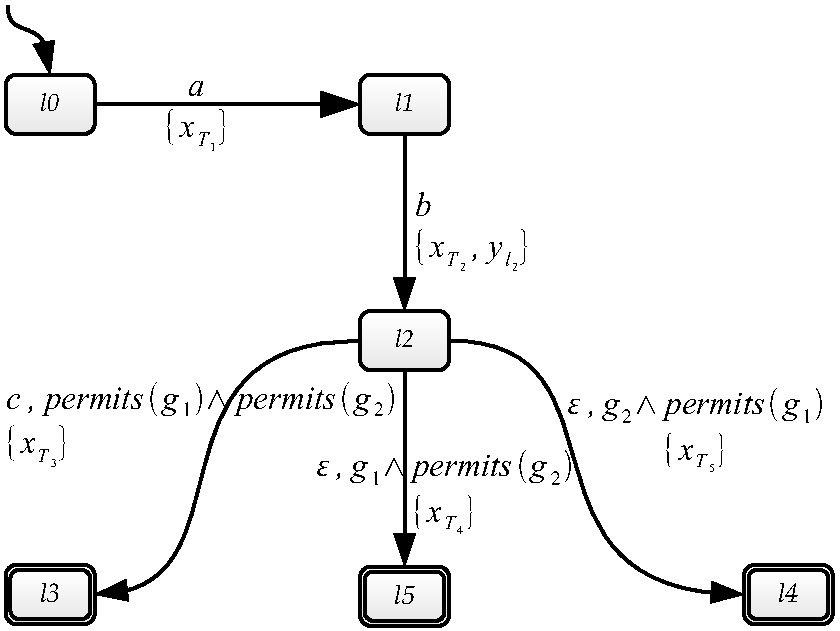
\includegraphics[width=\textwidth]{content/protocol-model/bogus-pta-constraint-fixed}
    \caption{A sample protocol timed automaton that does enforce M-Invoke semantics.}
    \label{fig:bogus-pta-constraint-fixed}
\end{figure}

The correct mapping of $\mathcal{P}$ to $A$ is given on Figure~\ref{fig:bogus-pta-constraint-fixed}, where the ``permits'' functions are just the cases that we mentioned above. For example, $\permits(g_1) = (x_{T_2} < 5) \bigvee x_{T_2} > 5) \wedge (x_{T_2} - y_{l_2} > 5)$.

% ........................................................................... %

\subsection{Protocol timed automata}

% ........................................................................... %

We named as \emph{protocol timed automata} the class of timed automata \cite{RADLD94} that we obtain by the mapping from a timed protocol that we illustrated informally in the previous section. They form a novel class of timed automata with the following characteristics:
\begin{enumerate}
  
  \item they support the empty word $\varepsilon$ as a switch label, and
  
  \item clocks are not freely added and reset on switches, they are instead split into two sets: one associates a unique clock to a unique switch while the second one associates a clock to every location that is the source of a $\varepsilon$-labeled switch, and
  
  \item the guards of $\varepsilon$-labeled switches must have at least one equality clause per possible disjunction (i.e., a clause of the form $(x = k)$ with $x$ being a clock and $k$ a rational constant or $\perp$), and
  
  \item they are deterministic, and
  
  \item the time domain is the set of positive reals $\Rpos$ augmented with the special symbol $\perp$\footnote{This symbol is used to denoted the fact that a clock is still at its initial value and has never been reset.}.
  
\end{enumerate}

The following definition gives the base of protocol timed automata. However, any automaton that satisfies this definition does not automatically enforce \MInvoke semantics. The techniques for doing that will be given later in this section.

\begin{definition}[Protocol timed automata]
Let $\T$ be the time domain defined as $\T = \Rpos \cup \{ \perp \}$.
A \emph{protocol timed automaton} $A$ is a timed automaton $A = (L, L^0, L^f, X \cup Y, E, \Sigma)$ over $\T$ such that $|L^0| = 1$ and the following conditions hold.

\begin{enumerate}

	\item For 2 switches $e = (l, g, a, r, l')$ and $e' = (l, g', a', r', l'')$ having the same source location $l$, either $a = a'$, or $g \wedge g' \models \mathtt{false}$.
	
	\item For every switch $e = (l, g, a, r, l')$, either:
	\begin{enumerate}

	 \item $l'$ is the source of a $\varepsilon$-labeled switch: $r = \{ x_e, y_{l'} \} $ with $x_e \in X$ being the clock attached to $e$ and $y_{l'} \in Y$ being the clock attached to $l'$, or
	 
	 \item $l'$ is not the source of a $\varepsilon$-labeled switch: $r = \{ x_e \} $ with  $x_e \in X$ being the clock attached to $e$.
	 
	\end{enumerate}
	It should be noted that the reset set of any switch is composed of 1 or 2 clocks.
	
	\item For every switch $e = (l, g, a, r, l')$ such that $a = \varepsilon$, $g$ is defined as a disjunction of conjunctive constraints having each at least one clock equality clause: $g = (x_1 = k_1 \wedge g_1') \vee \cdots \vee (x_n = k_n \wedge g_n')$ with $x_i$ being any clock, $k_i \in \Q \cup \{ \perp \}$ a rational constant or $\perp$, $n \in \N$ and $g_i'$ being any clocks constraint ($i \in \{1, \cdots, n \}$).

\end{enumerate}
\label{def:pta}
\end{definition}

% % ........................................................................... %
% 
% \subsection{Mapping}
% 
% % ........................................................................... %
% 
% We will use the timed protocol depicted on Figure~\ref{fig:pta-protocol} as a running example for presenting the mapping. This protocol exhibits two implicit transitions with their \MInvoke constraints.\\
% 
% We describe here how to map a timed protocol
% $$\mathcal{P} = (\mathcal{S}, s_0, \mathcal{F}, \mathtt{M}, \mathcal{X}, \mathcal{C}, \mathcal{R} \subseteq \mathcal{S}^2 \times \mathtt{M} \times \mathcal{C})$$
% to its corresponding protocol timed automaton
% $$A = (L, L^0, L^f, X \cup Y, E, \Sigma)$$
% The mapping makes use of several mapping functions, each being specialized in a portion of the mapping (e.g., one function is for states to locations, another one for transitions to edges and so on.).\\
% 
% We introduce the following mapping functions from elements of $\mathcal{P}$ to elements of $A$. Those functions are bijective.
% \begin{itemize}
%   
%   \item $\map_S: \mathcal{S} \longrightarrow L$ maps states to locations
%   
%   \item $\map_M: \mathtt{M} \longrightarrow \Sigma$ maps messages to input symbols
%   
%   \item $\map_C: \mathcal{X} \longrightarrow X$ maps transitions from $\mathcal{R}$ (each being identified by an element of $\mathcal{X}$) to clocks in $X$
%   
%   \item $\map_G: \mathcal{C} \longrightarrow \mathcal{C}(X \cup Y)$ maps temporal constraints\footnote{The notation $\mathcal{C}$ for timed protocols should not be confused with the notation $\mathcal{C}(X)$ in timed automata that denotes the set of constraints over a set of clocks $X$.} $\mathcal{C}$ of $\mathcal{P}$ to clock constraints over the set of clocks $X \cup Y$.
%   
% \end{itemize}
% 
% We now give the first step of the procedure to map $\mathcal{P}$ to $A$.
% 
% \begin{procedure}[Timed protocol mapping, step 1]
% $\mathcal{P}$ is mapped to $A$ as follows.
% \begin{enumerate}
%   
%   \item $L = \map_S(\mathcal{S})$
%   
%   \item $L^0 = \{ \map_S(s_0) \} $
%   
%   \item $L^f = \map_S(\mathcal{F})$
%   
%   \item $\Sigma = \map_M(\mathtt{M})$
%   
%   \item $X = \map_C(\mathcal{X})$
%   
%   \item For each transition $r = \mathcal{R}(s_1, s_2, m, c)$ identified by $T_{id} \in \mathcal{X}$, a switch $e = (\map_S(s_1), \map_G(c), \map_M(m), \{ \map_C(T_{id}) \}, \map_S(s_2))$ is added to $E$.
%   
% \end{enumerate}
% \label{proc:tp2pta}
% \end{procedure}
% 
% The mapping functions that we have introduced are straightforward. For example, a state $s \in \mathcal{S}$ is associated to a unique location $\map_S(s) \in L$. Similarly,
% $\map_G((T_1 < 3) || (T_2 > 4)) = (\map_C(T_1) < 3) \vee (\map_C(T_2) > 4)$. It should be noted that we allow abuse of notations such as using $\map_S$ over singletons (e.g, $\map_S(s)$) and sets (e.g., $\map_S(\mathcal{S})$).\\
% 
% At this step, the timed protocol of Figure~\ref{fig:pta-protocol} has been mapped to the timed automaton of Figure~\ref{fig:bogus-pta-constraint}. We can see how guards have been defined as well as a set of clocks. This is a relatively straightforward mapping.\\
% 
% This mapping definition is however not sufficient. Indeed, the \MInvoke constraints semantics are not enforced by the direct mapping through $\map_G$. Considering again the example on Figure~\ref{fig:bogus-pta-constraint},   the $c$-labeled switch has no guard (implicitly the guard is $g = \mathtt{true}$). If the guard of any of the $\varepsilon$-labeled switches is satisfied, then nothing actually forces it to be taken.

% ........................................................................... %

\subsection{Enforcing M-Invoke constraints in protocol timed automata}

% ........................................................................... %

We define the \MInvoke semantics so as to enforce that when the guard of a $\varepsilon$-labeled switch becomes satisfied, it is mandatorily taken. Indeed, classical timed automata augmented with $\varepsilon$-labeled switches only make the location change \emph{possible} when a guard is satisfied, not \emph{mandatory}.

\begin{definition}[\MInvoke semantics]
Let $A$ be a protocol timed automaton and $e: l \xrightarrow{\varepsilon, g} l'$ a $\varepsilon$-labeled switch of $A$. Let $v$ be the current clocks valuation such that:
\begin{enumerate}
  
  \item the current location is $l$, and
  
  \item $v \models g$
  
\end{enumerate}
In this case, the execution must immediately move to the location $l'$.
\end{definition}

Under \MInvoke semantics, the following behavior needs to be enforced (examples are taken from Figure~\ref{fig:bogus-pta-constraint}).
\begin{enumerate}
  
  \item When a $\varepsilon$-labeled switch guard becomes satisfied, all other switches must be immediately disabled so as to make it the only switch that can be taken. An example is when $g_1$ becomes satisfied in $l_2$: the two other switches must be disabled.
  
  \item When a location offering a $\varepsilon$-labeled switch is entered after the equality clause of its guard has been satisfied, the other switches must not be disabled. If $l_2$ is entered while $x_{T_2} > 5$, the other switches must not be disabled.
  
  \item When the guard of a $\varepsilon$-labeled switch cannot be satisfied when its equality clause is satisfied, the other switches must not be disabled. Let us consider $g_2$ while the current location is $l_2$. In case $(x_{T_1} = 10)$ is satisfied but $(x_{T_2} > 2)$ is not, the two other switches must not be disabled.
  
\end{enumerate}

The enforcement is done by rewriting the constraints using two functions. First, we define a function ``$\inhib$'' over a $\varepsilon$-labeled transition guard of the form $g = (x = k) \wedge g'$. The role of this function is to capture the cases where $g'$ is false, thus making the switch that has $g$ as its guard inactive. As we will see, this function plays a critical role in enforcing the \MInvoke constraints in protocol timed automata. Then, we will provide a function ``$\permits$'', also defined over a $\varepsilon$-labeled transition guard. It defines when it allows other switches from the same source location to become actionable. This function relies on the introduction of clocks that are attached to locations so as to capture the clocks valuation when locations are entered. It uses $\inhib$ that we introduce in the following definition.

\begin{definition}[$\inhib$ function]

Let a guard $g := (x = k) \wedge g'$ of a $\varepsilon$-labeled switch defined over a $\varepsilon$-labeled switch $l \rightarrow l'$ such as $x$ is a clock over $\T$, $k$ is a constant in $\Q \cup \{ \perp \}$ and $g'$ is any clocks constraint:
$ g' = 
(x_1 \;\#_1\; k_1) \wedge
 \cdots \wedge
 (x_j \;\#_j\; k_j) \wedge
 (x_{j+1} - x_{j+1}' \;\#_{j+1}\; k_{j+1}) \wedge
 \cdots \wedge
 (x_{m} - x_{m}' \;\#_{m}\; k_{m})
$
(for any $i \in \{1, \cdots, m\}$: $x_i, x_i' \in X \cup Y$, $k_i \in \Q \cup \{ \perp \}$ and $\;\#_i\;$ is any comparison operator).

We define the function $\inhib$ such that:
$
\inhib(g) =
  (x_1 - x \;\mathtt{not}(\#_1)\; k_1 - k) \vee 
  \cdots \vee 
  (x_j - x \;\mathtt{not}(\#_j)\; k_j - k) \vee
  (x_{j+1} - x_{j+1}' \;\mathtt{not}(\#_{j+1})\; k_{j+1}) \vee
  \cdots \vee 
  (x_{m} - x_{m}' \;\mathtt{not}(\#_{m})\; k_{m}) 
$

In the case where $g'$ is not defined (i.e., $g = (x = k)$), then $\inhib(g) = \mathtt{false}$.
\end{definition}

Going back to the timed automaton of Figure~\ref{fig:bogus-pta-constraint}:
$$
\left\lbrace
\begin{array}{l}
  \inhib(g_1) = \mathtt{false} \\
  \inhib(g_2) = (x_{T_2} - x_{T_1} \leq -8) \\
\end{array}
\right.
$$

Without loss of generality, we chose to reduce the $\varepsilon$-labeled switch guard $g$ to a unique conjunction in the previous definition to simplify the notations. The case where $g$ is a disjunction is easy: we consider it as multiple $\varepsilon$-labeled switches with each switch having a single conjunctive guard. We keep this assumption in the remainder.\\

With this $\inhib$ function at hand, we can now define a function called $\permits$. When given the guard of a $\varepsilon$-labeled switch, it defines when the other switches from the same source location can be enabled without contradicting M-Invoke constraints.

\begin{definition}[$\permits$ function]
  
Let a guard $g := (x = k) \wedge g'$ of a $\varepsilon$-labeled switch defined over a $\varepsilon$-labeled switch $l \rightarrow l'$ such as $x$ is a clock over $\T$, $k$ is a constant in $\Q \cup \{ \perp \}$ and $g'$ is any clocks constraint. Let $y \in Y$ the clock that is commonly reset by all the switches whose target location is $l$. We define the following clauses:
\begin{enumerate}
  
  \item $S_1 = (x < k)$
  
  \item $S_2= (x > k) \wedge (x - y > k)$
  
  \item $S_3 = (x > k) \wedge (x - y \leq k) \wedge \inhib(g)$
  
  \item $S_4 = (x = k) \wedge \inhib(g)$
  
\end{enumerate}

The function $\permits(g)$ is defined as
$$
  \permits(g) = \bigvee\limits_{i \in \{1, 2, 3, 4\}} S_i
$$
  
\end{definition}

The $\permits$ function disjunctive clauses play the following roles. $S_1$ captures the cases where the current clocks valuation $v$ ensures that $v(x)$ is still below $k$. $S_2$ captures the cases where $v$ is above $k$ and the location $l$ has been entered after $(x = k)$ was satisfied. This is checked through the clause $(x - y > k)$. $S_3$ captures the cases where $l$ was entered before $(x = k)$ was satisfied, but $g_i'$ could not be satisfied. In such cases, the switches should not be disabled for the clocks valuations such that $(x > k)$ is satisfied. Finally, $S_4$ captures the cases where $(x = k)$ is satisfied but $g_i'$ is not, hence the switches don't have to be disabled as well.\\

Again considering the timed automaton of Figure~\ref{fig:bogus-pta-constraint}:
$$
\left\lbrace
\begin{array}{lll}
  
  \permits(g_1) & =    & \underbrace{(x_{T_2} < 5)}_{S_1} \\
                & \bigvee & \underbrace{(x_{T_2} > 5) \wedge (x_{T_2} - y_{l_2} > 5)}_{S_2} \\
  
  \permits(g_2) & =    & \underbrace{(x_{T_1} < 10)}_{S_1} \\
                & \bigvee & \underbrace{(x_{T_1} > 10) \wedge (x_{T_1} - y_{l_2} > 10)}_{S_2} \\
                & \bigvee & \underbrace{(x_{T_1} > 10) \wedge (x_{T_1} - y_{l_2} \leq 10) \wedge
                            \underbrace{(x_{T_2} - x_{T_1} \leq -8)}_{\inhib(g_2)}}_{S_3} \\
                & \bigvee & \underbrace{(x_{T_1} = 10) \wedge
                            \underbrace{(x_{T_2} - x_{T_1} \leq -8)}_{\inhib(g_2)}}_{S_4} \\
  
\end{array}
\right.
$$

We can now define how the guards of the switches whose source locations offer $\varepsilon$-labeled switches need to be rewritten so as to enforce \MInvoke.

\begin{procedure}[\MInvoke enforcement]
  
Let $l$ be a location of a protocol timed automaton $A$ that offers $n > 0$ $\varepsilon$-labeled switches:
$$ \{
  e_{\varepsilon_1} = (l, g_{\varepsilon_1}, \varepsilon, r_1, l_1),
  \cdots,
  e_{\varepsilon_n} = (l, g_{\varepsilon_n}, \varepsilon, r_n, l_n)
\} $$ 

The rewriting of the guard of each switch whose source location is $l$ (including the $\varepsilon$-labeled ones) is performed as follows:
\begin{enumerate}
  
  \item for each location $l$ that offers a $\varepsilon$-labeled switch, augment the reset set of each switch whose target location is $l$ with the clock $y_l \in Y$
  
  \item compute $\{ \permits(g_{\varepsilon_1}), \cdots \permits(g_{\varepsilon_n}) \}$
  
  \item rewrite the guard $g$ of each switch $(l, g, a, r, l')$ as
  \begin{enumerate}
  	\item when $a \neq \varepsilon$
  		$$ g \bigwedge\limits_{0 \leq i \leq n} \permits(g_{\varepsilon_i})$$
  	\item when $a = \varepsilon$ and the switch guard is $g_{\varepsilon_j}$ ($j \in \{1, \cdots, m\}$)
  		$$ g \bigwedge\limits_{0 \leq i \neq j \leq n} \permits(g_{\varepsilon_i}) $$
  \end{enumerate}
  
\end{enumerate}
\label{proc:guard-rewrite}
\end{procedure}

As an example, we consider again the protocol timed automaton of Figure~\ref{fig:bogus-pta-constraint} that has been fixed to enforce M-Invoke semantics on Figure~\ref{fig:bogus-pta-constraint-fixed}.

% ........................................................................... %

\subsection{Theoretical results}

% ........................................................................... %

We now study the expressiveness of protocol timed automata, then prove that the mapping from timed protocols to timed automata is correct.

\subsubsection{Expressiveness}

\begin{theorem}
$\varepsilon$-transitions strictly increase the expressiveness of protocol timed automata.
\label{thm:mi-expressiveness}
\end{theorem}

\begin{figure}[htbp]
  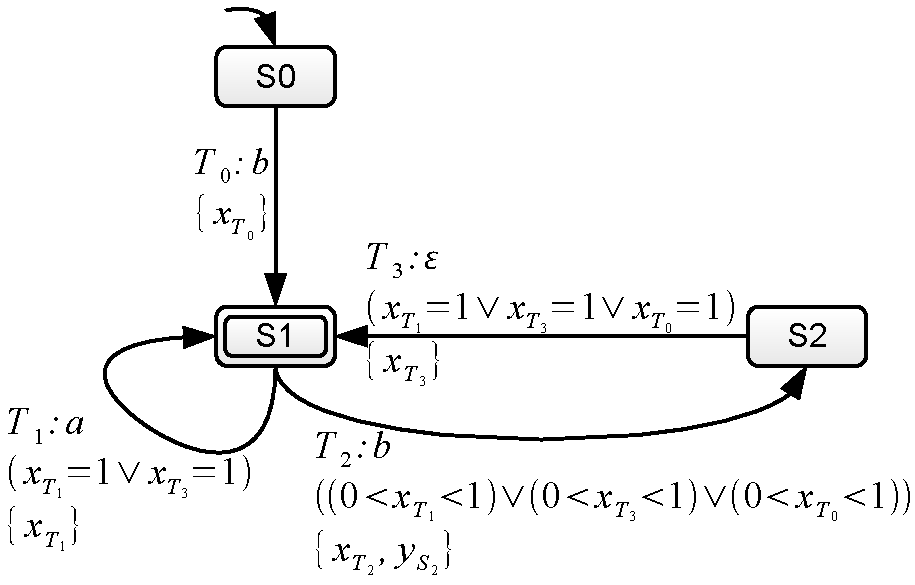
\includegraphics[width=\textwidth]{content/protocol-model/precise-time}
  \caption{A protocol timed automaton $A$ that cannot be expressed equivalently without $\varepsilon$-transitions.}
  \label{fig:precise-time}
\end{figure}

Protocol timed automata are strictly more expressive than (general) timed automata because of their $\varepsilon$-labeled switches. The proof, given on page~\pageref{proof:mi-expressiveness}, is based on the notion of \emph{precise actions} and is the same as Corollary~29 of \cite{BBVD+99}. The idea is that the protocol timed automaton of Figure~\ref{fig:precise-time} cannot be expressed equivalently by a timed automaton without $\varepsilon$-labeled switches.

\subsubsection{Correctness of the mapping}

We now give some results showing that the guards rewritings above are correct with respect to the M-Invoke constraint semantics. Indeed, the correctness of the mapping from timed protocols to protocol timed automata relies on the rewriting to correctly enforce \MInvoke constraints semantics. The following lemma shows that the function $\inhib$ works as expected, i.e., it can inhibit guards when a $\varepsilon$-labeled switch guard is totally satisfied, and allow them when it is not. The proof is given on page~\pageref{proof:inhib}.

\begin{lemma}
Let a protocol timed automaton $A$ and a location $l \in A$ such that there exists a switch $e = (l, g = (x = k) \wedge g', \varepsilon, r, l')$, with
$g' = 
(x_1 \;\#_1\; k_1) \wedge
 \cdots \wedge
 (x_j \;\#_j\; k_j) \wedge
 (x_{j+1} - x_{j+1}' \;\#_{j+1}\; k_{j+1}) \wedge
 \cdots \wedge
 (x_{m} - x_{m}' \;\#_{m}\; k_{m})$ for $m \in \N$ and $j \in \{1, \cdots, m\}$. Then:
\begin{enumerate}

  \item $(\inhib(g) = \mathtt{true}) \Longrightarrow (g' = \mathtt{false})$
  
  \item $(\inhib(g) = \mathtt{false}) \Longrightarrow (g' = \mathtt{true})$

\end{enumerate}
\label{lemma:inhib}
\end{lemma}

Given a location that has several $\varepsilon$-labeled switches, the following lemma checks that only one of them can ever become satisfied, thus disabling and forcing the transition to another location. To do that, we express the following sanity-check type of boolean implication. A proof is given on page~\pageref{proof:permits}.

\begin{lemma}
Let a protocol timed automaton $A$ and a location $l \in A$ such that it offers $n > 0$ $\varepsilon$-labeled switches. For any $i \in \{1, \cdots, n\}$, the guard $\widetilde{g_i}$ of the $i$-th $\varepsilon$-labeled switch is of the form
$$g_i \bigwedge\limits_{1 \leq i \neq j \leq n} \permits(g_j)$$

Let $i \in \{1, \cdots, n \}$ and $j \in \{1, \cdots, n\}$ such that $i \neq j$. Then:
$$
(g_j = \mathtt{true}) \Longrightarrow (\permits(g_j) = \mathtt{false}) \wedge (\permits(g_i) = \mathtt{true})
$$
\label{lemma:permits}
\end{lemma}

This implication expresses the fact that when a $\MInvoke$ guard is satisfied, then its derived $\permits$ constraint is false, and the permits clauses of every other $\MInvoke$ guards are still true. Indeed, if any of the later permits clauses was to be false, then it would mean that its guard would have already been actionable in the past, yet not taken and hence not enforced.\\

The following theorem states that the mapping of a timed protocol to a protocol timed automaton is correct with respect to \MInvoke constraints. The proof is given on page~\pageref{proof:mi-enforcement}.

\begin{theorem}
Let a protocol timed automaton $A$ obtained from a timed protocol $\mathcal{P}$ on which Procedure~\ref{proc:guard-rewrite} has been applied.
Every $\varepsilon$-labeled switch $e = (l, g = (x = k) \wedge g', \varepsilon, r, l')$ of $A$ is taken as soon as its guard $g$ is satisfied.
\label{thm:mi-enforcement}
\end{theorem}

Finally, the following lemma states that protocol timed automata are deterministic. The proof is given on page~\pageref{lemma:pta-determinism}.

\begin{lemma}
Protocol timed automata are deterministic: given a protocol timed automaton $A$ and a timed word $w \in \mathcal{L}(A)$, $w$ has exactly one run over $A$.
\label{lemma:pta-determinism}
\end{lemma}

% ........................................................................... %

\section{Discussion}

% ........................................................................... %

The following discussion aims at first positioning protocol timed automata with respect to event-clock automata as defined in \cite{RALF94}. We then discuss two potential limitations in our model. The first is the absence of support for absolute time constants (e.g., supporting constraints of the form $(x < \mbox{\texttt{2008-05-10:20:00:00}})$). The second one is the assumption that we do not take into account network transport delays and losses. 

% ........................................................................... %

\subsection{Relationship to event-clock automata}

% ........................................................................... %

The class of protocol timed automata can be seen as an extension of event-recording automata \cite{RALF94}. In fact, their design has been made with them in mind. Yet, any protocol timed automaton is not necessarily a event-recording automaton. One straightforward similarity between the two classes is the time domain $\T = \Rpos \cup \{ \perp \}$ and that clocks are assigned and reset in a restricted fashion. There are however several differences:
\begin{itemize}
  
  \item protocol timed automata support $\varepsilon$-labeled switches with clock resets, and
  
  \item some particular switches may reset two clocks (i.e., the ones whose target location offers a $\varepsilon$-labeled switch), and
  
  \item one subset of the clocks assigns them to switches (i.e., $X$), not input symbols, while the complement subset assigns them to locations ($Y$).
  
\end{itemize}

However as we will see in the next chapters, protocol timed automata are fully deterministic, and they have the property that the value of clocks only depends of the input words, despite $\varepsilon$-labeled switches (at first sight, one would think that they necessarily introduce indeterminism).\\

The class of event-recording automata is however a subset of protocol timed automata. Indeed, let us consider an event-recording automaton: it can be translated directly to a protocol timed automaton $A$ as:
\begin{enumerate}
  
  \item there is no $\varepsilon$-labeled switch, and
  
  \item for every input symbol $a$ and any guard clause of the form $(x_a \;\#\; k)$ ($\#$ is any operator and $k$ a constant), it can be rewritten as $(x_{e1} \;\#\; k) \vee \cdots \vee (x_{en} \;\#\; k)$ where $\{ x_{e1}, \cdots, x_{en} \}$ is the set of switches in $A$ where $a$ is the input symbol.
  
\end{enumerate}

\begin{figure}[htbp]
	\centering
  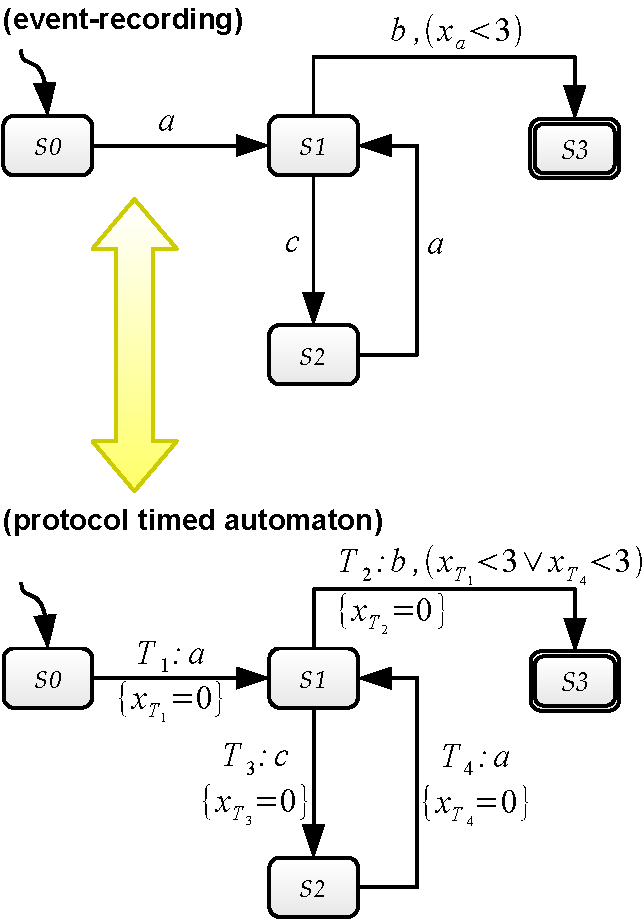
\includegraphics[width=0.7\textwidth]{content/protocol-model/era}
  \caption{A sample event-recording automaton viewed as a protocol timed automaton.}
  \label{fig:era}
\end{figure}

We give an example on Figure~\ref{fig:era} of a event-recording timed automaton encoded as a protocol timed automaton.

% ........................................................................... %

\subsection{Constraints with absolute dates}

% ........................................................................... %

Timed protocol constraints are always expressed relatively to a transition of a given protocol being fired (e.g., $\CInvoke(T_1 < 3h)$). Absolute dates cannot be used in constraints (e.g., $\CInvoke(T_1 < \mbox{'2007-04-19 14:49:00'})$ or $\CInvoke(\mbox{current\_time} < \mbox{'2007-04-19 14:49:00'})$). Such types of constraints can be found in some specifications such as BPEL \cite{WSBPEL2} where both types of \emph{relative} and \emph{absolute} time expressions can be used.\\

Let us briefly investigate the impact of introducing absolute dates into the model by looking at the involved mechanisms at the timed automata level. Allowing a constraint to compare a clock $x$ to a constant $date$ (e.g., $x < \mbox{'2007-04-19 14:49:00'}$) which represents an absolute date requires the following assumptions.
\begin{enumerate}
    \item $x$ is set to a constant $now$ which represents the current date when the automaton execution starts, and
    \item $x$ is always compared to absolute dates, and
    \item $x$ is never reset in the considered automaton.
\end{enumerate}

We claim that making such an extension renders the timed language emptiness checking problem undecidable. The proof can be done by observing that $now$ is actually a variable. In timed automata, the clocks are set to a constant value (usually $0$) when the execution starts. Here, we would have some special clocks that would be initially set to a value which depends on the current time. Hence, the result of checking for the emptiness of such an extended timed automaton would only hold considering the time at which the checking has been performed (i.e., the results holds at time $t$ but may not hold anymore at time $t + \delta$ with any $\delta \in \Rpos$).\\

This limitation of timed protocols in terms of expressiveness is not a penalty as such constructs are of limited use in practice. In the case of BPEL, timers are mainly used for generating timeout exceptions in asynchronous operations (e.g., the \emph{pick} complex activity). They can be also used for a \emph{wait} activity (e.g., put the process in sleep). In our experience, we have never found a need for expressing absolute dates in BPEL processes. Also, \emph{JBoss JBPM} (see \url{http://www.jboss.com/products/jbpm}), a widely used business process management system, offers a workflow language called \emph{jPDL} where time-related constructs are always expressed in a relative manner (i.e., \emph{jPDL} does not allow specifying absolute dates for timers).

% ........................................................................... %

\subsection{Message transport communications}

% ........................................................................... %

Our model is based on the assumption that there are no message transmission delays and losses. This is of course not the case in reality as web services messages are mostly transported over unreliable networks that can have substantial load variations, leading to greatly varying network latencies and even errors. The class of \emph{Robust Timed Automata} \cite{RAPM04} is a possible exploration path for solving those issues. Briefly, a robust timed automaton recognizes timed words with some fuzziness in the event dates as no real world system can be expected to be as precise as timed automata expectations. The classical decidability problems (reachability / emptiness, inclusion) remain unchanged for this class. However, the expressiveness of such automata cannot be compared to the one of timed automata \cite{RAPM04}. That is why we guess that using them as a formal framework for timed protocols probably requires substantial investigations from a theoretical point of view.

% % ........................................................................... %
% 
% \subsection{Inverse mapping: from protocol timed automata back to timed protocols}
% 
% % ........................................................................... %
% 
% Given a protocol timed automaton
% $$A = (L, L^0, L^f, X \cup Y, E, \Sigma)$$
% its corresponding timed protocol
% $$\mathcal{P} = (\mathcal{S}, s_0, \mathcal{F}, \mathtt{M}, \mathcal{X}, \mathcal{C}, \mathcal{R} \subseteq \mathcal{S}^2 \times \mathtt{M} \times \mathcal{C})$$
% can easily be obtained as follows. The construction is relatively easy given the mapping described in Procedure~\ref{proc:tp2pta}, hence we will keep the discussion rather informal.\\
% 
% The mapping functions used in Procedure~\ref{proc:tp2pta} support direct inverse functions. For example the mapping from locations in $A$ to states in $\mathcal{P}$ is given by
% $$ \map_S^{-1}: L \longrightarrow \mathcal{S} $$
% that associates to each location a location in $\mathcal{S}$.\\
% 
% The inverse mapping requires two preliminary steps:
% \begin{enumerate}
%   
%   \item remove the $\permits$ clauses from the guards in $A$, then
%   
%   \item remove the set of clocks $Y$ in $A$ (these clocks are only used in $\permits$ clauses).
%   
% \end{enumerate}
% When this is done, the inverse mapping functions can be applied to infer a timed protocol.\\
% 
% Consider the protocol timed automaton of Figure~\ref{fig:bogus-pta-constraint-fixed}. The first two steps presented below yield the timed automaton of Figure~\ref{fig:bogus-pta-constraint}. Applying inverse functions gives back the timed protocol first introduced on Figure~\ref{fig:pta-protocol}.

% ........................................................................... %

\chapter{Protocol analysis}
\label{chap:protocol-analysis}
% ........................................................................... %

Timed protocols can be used to model the external behaviors of web services interfaces by capturing the messages choreographies as well as the timing constraints that are put on them. We focus now on the analysis of timed protocols given the following two dimensions: compatibility and replaceability. To do that, we introduce for each type a set of analysis flexible classes. By flexible, we mean that those classes cater for more than ``black or white'' compatibility or replaceability cases like it has been traditionally done for hardware and software components. For example one may look for compatibility or replaceability only for a limited subset of a provider or requester protocol specification.\\

This chapter is structured as follows. We first present compatibility then replaceability analysis before turning our attention to a set of timed protocol operators that can be combined to characterize those classes. The approach that is presented here extends the one from \cite{FTBB} with timing constraints being added to the business protocol model.

% ........................................................................... %

\section{Classes of protocol-based analysis}

% ........................................................................... %

We start this chapter by presenting compatibility then replaceability analysis.

% ........................................................................... %

\subsection{Protocol-level compatibility}

% ........................................................................... %

Compatibility analysis is concerned with verifying whether two services can interoperate. It is necessary for both static and dynamic binding, and it also aids in managing evolution as it helps verify that a modified client can still interact with a certain service.\\

More precisely, we identified two compatibility classes.
\begin{enumerate}

	\item Partial compatibility between two protocols $\mathcal{P}_1$ and $\mathcal{P}_2$ implies that at least one conversation can be carried out between two services implementing these protocols.

  \item A protocol $\mathcal{P}_1$ is \emph{fully compatible} with $\mathcal{P}_2$ if $\mathcal{P}_2$ can support all message exchanges that $\mathcal{P}_1$ can generate (the inverse is not necessarily true).

\end{enumerate}\

Ideally, if we have developed a service $S$ characterized by protocol $\mathcal{P}$, at binding time we will want to look for services that have a protocol with which $\mathcal{P}$ is fully compatible, so that every message exchange that our service can generate is understood by our partner.\\

\begin{figure}[thbp]
    \centering
    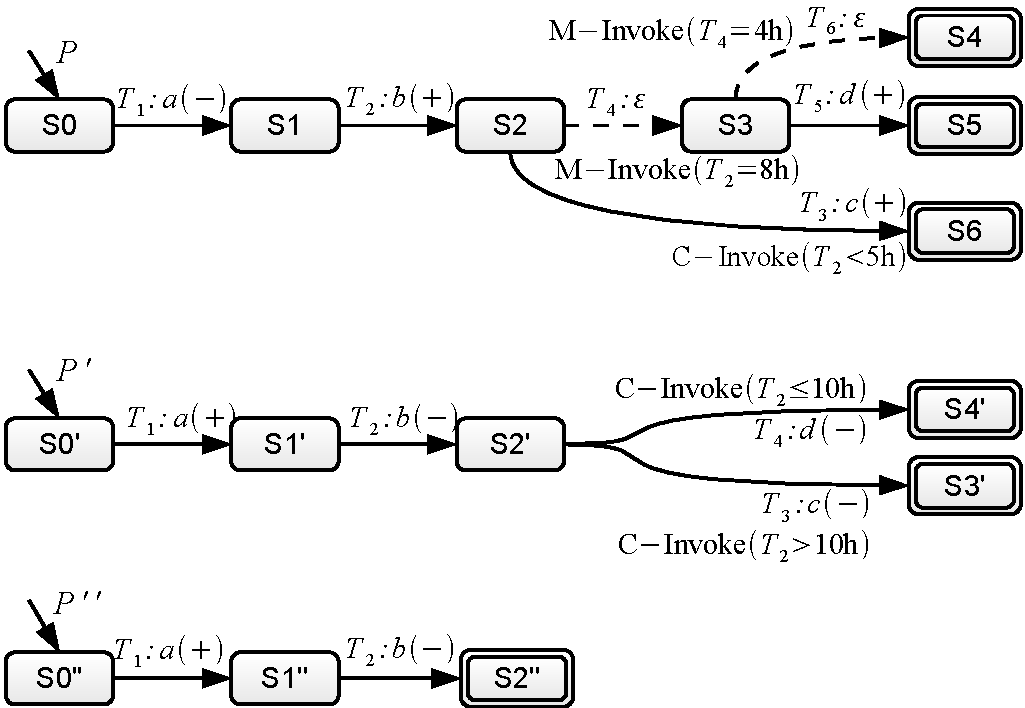
\includegraphics[width=\textwidth]{content/protocol-analysis/analysis}
    \caption{Three protocols for illustrating protocol analysis.}
    \label{fig:analysis}
\end{figure}

We illustrate compatibility analysis with respect to timing constraints and its challenges on the examples below.
Let us consider the protocols $\mathcal{P}$ and $\mathcal{P'}$ depicted on Figure~\ref{fig:analysis}. Without the time constraints, we can observe that $\mathcal{P}$ is fully compatible with $\mathcal{P'}$: $a \cdot b \cdot c$ and
$a \cdot b \cdot d$ are valid interaction traces of the untimed versions of $\mathcal{P}$ and $\mathcal{P'}$. However, due to the \CInvoke constraints specified on transition $T_3$ of each protocol, $\mathcal{P}$ and $\mathcal{P'}$ cannot interact correctly. Indeed, $\mathcal{P}$ supports timed conversations of the form $(a(-), 0) \cdot (b(+), t) \cdot (c(+), t')$ (with $t' < t + 5$), while $\mathcal{P'}$ supports timed conversations of the form $(a(+), 0) \cdot (b(-), t) \cdot (c(-), t')$ (with $t' > t + 10$). Hence, these two protocols cannot interact correctly since $\mathcal{P'}$ will always send a message $c$ later than $\mathcal{P}$ allows it to be received. Therefore, two protocols must agree on the ordering of the exchanged messages as well as on the time constraints to be compatible.\\

Let us now consider the protocols $\mathcal{P}$ and $\mathcal{P''}$ on Figure~\ref{fig:analysis}. When interacting according to the timed interaction trace $(a, 0) \cdot (b, t)$, $\mathcal{P}$ moves to a non-final state $s_2$ while $\mathcal{P''}$ moves to a final state  $s_2''$, ending the conversation from its side. However, due the presence of the implicit transitions $T_4$ and $T_5$, $\mathcal{P}$ is able to terminate correctly its execution by moving automatically to the final state $s_4$: it waits at state $s_2$ for $8$ hours, then moves to $s_3$ where it waits for $4$ hours before finally moving to $s_4$ which is a final state. Therefore, $\mathcal{P}$ and $\mathcal{P''}$ can interact correctly following the interaction trace $(a, 0) \cdot (b, t)$.\\

The last example shows that the implicit transitions have an impact on the identification of the final states, naturally impacting the compatibility analysis. We consider again $\mathcal{P}$ and $\mathcal{P'}$ from Figure~\ref{fig:analysis}.
After exchanging the messages $a$ and $b$, the two protocols move to the states $s_2$ and $s_2'$ respectively. If we consider the explicit operations that are available from these two states, $s_2'$ provides an operation $d(-)$ while $s_2$ does not enable any invocation of a $d$ message receiving operation. As a consequence, focusing the compatibility checking only on these two states is not enough. Indeed, the presence of the implicit transition $T_4$ in $\mathcal{P}$ moves automatically a service conversation to the state $s_3$ after $8$ hours from when $d$ can be received. Hence, $\mathcal{P}$ and $\mathcal{P'}$ can interact correctly by following timed interactions traces of the form $(a, 0) \cdot (b, t) \cdot (c, t')$, with $t + 8 < t' \leq t + 10$ (i.e., if the message $d$ is sent between $8$ and $10$ hours after the message $b$).

% ........................................................................... %

\subsection{Protocol-level replaceability}

% ........................................................................... %

Replaceability analysis identifies whether a service can acts as a substitute of another one, either in general or when interacting with certain requesters. Such an analysis involves finding the set of conversations that both services can support even if they are not equivalent. This is useful, for example, to determine whether a new version of a service (protocol) can support the same conversations as the previous one or whether a newly defined service can support the conversations that a given standard specification mandates.\\

As in the case of compatibility, we identified several replaceability classes.
\begin{enumerate}

	\item \emph{Protocol equivalence} occurs when two protocols support exactly the same conversations.
	
	\item \emph{Protocol subsumption} occurs when a protocol supports at least all of the conversations of another one.
	
	\item \emph{Protocol replaceability w.r.t. a client protocol} occurs when a protocol $\mathcal{P}_1$ can replace a protocol $\mathcal{P}_2$ when interacting with a client protocol $\mathcal{P}_c$ if every valid conversation between $\mathcal{P}_2$ and $\mathcal{P}_c$ is also a valid conversation between $\mathcal{P}_1$ and $\mathcal{P}_c$. This latter definition is helpful in managing evolution, as when we update our service we may want to check that it can still communicate with the same clients it was interacting before.
	
	\item \emph{Protocol replaceability w.r.t. an interaction role} is similar to the previous one. It occurs when a protocol $\mathcal{P}_1$ can replace a protocol $\mathcal{P}_2$ if $\mathcal{P}_1$ behaves like $\mathcal{P}_2$ when $\mathcal{P}_2$ behaves as an interaction role $\mathcal{P}_r$.

\end{enumerate}

For all of the above classes, we can distinguish between full and partial replaceability. Full replaceability is as defined above. Partial replaceability is when there is replaceability but only for some conversations. As an example, we have a partial replaceability with respect to a client protocol when a protocol $\mathcal{P}_1$ can replace another protocol $\mathcal{P}_2$ in at least one conversation that can occur with $\mathcal{P}_c$.\\

To illustrate replaceability, let us consider a protocol $\mathcal{P}_1$ obtained from the protocol $\mathcal{P''}$ on Figure~\ref{fig:analysis} by reversing the polarities of the messages. Such a protocol can be replaced by $\mathcal{P}$ on Figure~\ref{fig:analysis}. Indeed, the only timed conversation supported by  $\mathcal{P}_1$ are of the form $(a(-), 0) \cdot (b(-), t)$ (with $t > 0$) and such  conversations are also supported by  $\mathcal{P}$. The opposite is however not true because for example $\mathcal{P}$ may support some conversations that contain the messages $c$ or $d$, while $\mathcal{P}_1$ does not. Interestingly, we can observe that $\mathcal{P}_1$  can replace $\mathcal{P}$ when interacting with $\mathcal{P''}$: the only timed conversations of $\mathcal{P}$ that are understood by $\mathcal{P''}$ are of the form $(a(-), 0) \cdot (b(-), t)$ (with $t > 0$) and which are also supported by $\mathcal{P}_1$.\\

The next section presents a set of timed protocol operators that can be used to completely characterize the above compatibility and replaceabilty classes.

% ........................................................................... %

\section{Protocol operators}

% ........................................................................... %

We split the set of protocol operators in two categories: \emph{manipulation} and \emph{comparison} operators. The former category allows to compute protocols capturing properties regarding a pair of protocols, for example to compute a protocol that captures all of the common timed conversations of two protocols. The later category allows to compare two protocols for subsumption ($\sqsubseteq$) and equivalence ($\equiv$). We informally describe the protocol manipulation operators below, while their formal semantics are presented in Table~\ref{tab:operators}.

\begin{definition}[Timed protocol operators]
~
\begin{description}

  \item[Parallel composition] ($\compop$) takes two input timed protocols and returns a \emph{timed interaction protocol} that captures the possible interactions between them. A timed interaction protocol has simply no messages polarities. More precisely, the resulting timed interaction protocol describes the set of timed interaction traces of the input protocols.

  \item[Projection] is used to project the polarity of one protocol on the parallel composition of two protocols, and is denoted as $\projop{\mathcal{P}_1}{\mathcal{P}_2}{\mathcal{P}_1}$.

  \item[Intersection] ($\intersop$) takes two input timed protocols and returns one timed protocol that captures the timed conversations that they have in common.

  \item[Difference] ($\diffop$) takes two input timed protocols and returns one that captures the timed conversations that are supported by the first input protocol but not by the second one.
  
  \item[Subsumption] ($\sqsubseteq$) tests whether one protocol supports all of the timed conversations of another protocol (i.e., $\mathcal{P} \sqsubseteq \mathcal{P'}$ if and only if $Tr(\mathcal{P}) \subseteq Tr(\mathcal{P'})$).
  
  \item[Equivalence] ($\equiv$) checks whether two timed protocols support exactly the same set of timed conversations (i.e., $\mathcal{P} \equiv \mathcal{P'}$ if and only if $Tr(\mathcal{P}) = Tr(\mathcal{P'})$. 

\end{description}
\end{definition}

\begin{table}[thbp]
{\footnotesize
\begin{center}
\begin{tabular}{|p{2.5cm}|p{1.2cm}|p{8.3cm}|}
%
\hline
%
\textbf{Operator name} & \textbf{Symbol} &  \textbf{Semantics}\\ \hline
%
Compatible Composition & $\compop$  & $\mathcal{P} = \mathcal{P}_1 \compop \mathcal{P}_2$ is a protocol $\mathcal{P}$ such that
$T \in Tr(\mathcal{P})$ iff  $T$  is an interaction trace of  $\mathcal{P}_1$ and $\mathcal{P}_2$ \\ \hline
%
Intersection  & $\intersop$ & $\mathcal{P} = \mathcal{P}_1 \intersop \mathcal{P}_2$ is a protocol $\mathcal{P}$ such that
$Tr(\mathcal{P}) =  Tr(\mathcal{P}_1) \cap Tr(\mathcal{P}_2)$ \\ \hline
 %
Difference  & $\diffop$ & $\mathcal{P} = \mathcal{P}_1 \diffop \mathcal{P}_2$ is a protocol $\mathcal{P}$ that satisfies the following condition:
$Tr(\mathcal{P}) = Tr(\mathcal{P}_1) \setminus Tr(\mathcal{P}_2) $  \\ \hline
 %
 Projection & $\projop{}{}{}$ &  Let $\mathcal{P} = \mathcal{P}_1 \compop \mathcal{P}_2$. $\projop{\mathcal{P}_1}{\mathcal{P}_2}{\mathcal{P}_i}$, with $i \in \{1, 2\}$,
is the protocol  obtained from $\mathcal{P}_1 \compop \mathcal{P}_2$
by defining  the polarity function of the messages as follows: $Polarity(\projop{\mathcal{P}_1}{\mathcal{P}_2}{\mathcal{P}_i}, m) = Polarity(\mathcal{P}_i, m), \forall m \in \mathtt{M}$ \\ \hline
 %
\end{tabular}
\caption{Protocol manipulation operators semantics.}
\label{tab:operators}
\end{center}
}
\end{table}

\begin{figure}[thbp]
    \centering
    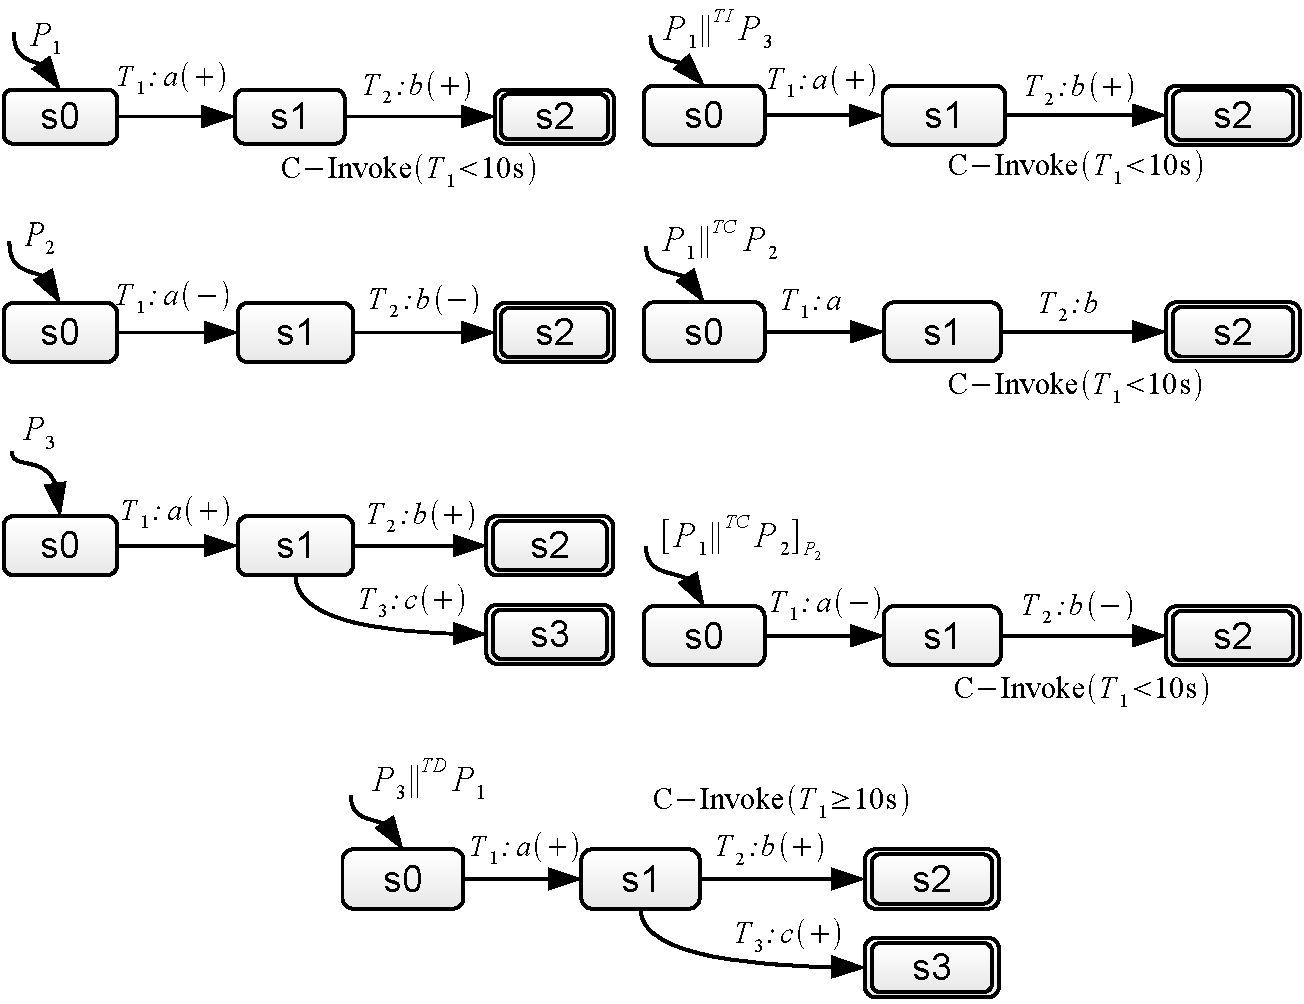
\includegraphics[width=\textwidth]{content/protocol-analysis/operators}
    \caption{Three timed protocols $\mathcal{P}_1, \mathcal{P}_2$ and $\mathcal{P}_3$ and some resulting protocols when using protocol manipulation operators.}
    \label{fig:operators}
\end{figure}

To illustrate these operators, Figure~\ref{fig:operators} shows three simple timed protocols $\mathcal{P}_1$, $\mathcal{P}_2$ and $\mathcal{P}_3$ as well as some results when applying operators on them.
For example, the protocol $\mathcal{P}_1 \intersop \mathcal{P}_3$ captures the timed conversations that are commonly supported by both $\mathcal{P}_1$ and $\mathcal{P}_3$: $\mathcal{P}_1$ does not support receiving a message $c$, hence it does not appear in $\mathcal{P}_1 \intersop \mathcal{P}_3$. Similarly $\mathcal{P}_1$ can only receive a $b$ message within the 10 seconds that follow the reception of a $a$ message. Another example is the protocol $\mathcal{P}_3 \diffop \mathcal{P}_1$ that captures all of the conversations that $\mathcal{P}_3$ supports but that $\mathcal{P}_1$ doesn't support. This is why the \CInvoke constraint of $T_2$ in $\mathcal{P}_3 \diffop \mathcal{P}_1$ is the negation of the one of $T_2$ in $\mathcal{P}_1$ as $\mathcal{P}_3$ does not carry a \CInvoke constraint on its transition $T_2$. Similarly, $\mathcal{P}_3$ supports receiving $c$ messages while $\mathcal{P}_1$ does not. Finally, the protocol $\mathcal{P}_3$ on Figure~\ref{fig:operators} subsumes the protocol $\mathcal{P}_1$.

% ........................................................................... %

\section{Characterizing the compatibility and replaceability classes}

% ........................................................................... %

Based on the operators introduced above, the following lemma gives the necessary and sufficient conditions to identify the compatibility level between two timed protocols.

\begin{lemma}
Let $\mathcal{P}_1$ and $\mathcal{P}_2$ be two timed business protocols.
\begin{enumerate}

    \item $\mathcal{P}_1$ and $\mathcal{P}_2$ are \emph{partially compatible} iff $\mathcal{P}_1 \compop \mathcal{P}_2$ is not an empty protocol (i.e., $Tr(\mathcal{P}_1 \compop \mathcal{P}_2) \neq \emptyset)$).

    \item $\mathcal{P}_1$ and $\mathcal{P}_2$ are \emph{fully compatible} iff $\projop{\mathcal{P}_1}{\mathcal{P}_2}{\mathcal{P}_1} \equiv \mathcal{P}_1$.

\end{enumerate}
\end{lemma}

Indeed, if a timed interaction protocol resulting from a compatible composition of two input protocols is not empty, it means that there is at least one timed interaction trace between the input protocols, and hence these protocols are compatible. Otherwise, the input protocols are not compatible. Regarding the second item of the lemma, the projection $\projop{\mathcal{P}_1}{\mathcal{P}_2}{\mathcal{P}_1}$ describes all the timed conversations of $\mathcal{P}_1$ that are also understood by $\mathcal{P}_2$. As a consequence, if such a set of conversations contains all the ones of $\mathcal{P}_1$, it implies that $\mathcal{P}_1$ is fully compatible with $\mathcal{P}_2$. Otherwise, $\mathcal{P}_1$ is not fully compatible with $\mathcal{P}_2$ since there is at least one timed conversation of $\mathcal{P}_1$ which cannot be understood by $\mathcal{P}_2$.\\

The following lemma characterizes the replaceability levels of two given protocols using the operators introduced in the previous section.

\begin{lemma}
Let $\mathcal{P}_1$, $\mathcal{P}_2$, $\mathcal{P}_C$ and $\mathcal{P}_R$ be three timed business protocols.
\begin{enumerate}

    \item $\mathcal{P}_1$ can \emph{replace} $\mathcal{P}_2$ iff $\mathcal{P}_2 \sqsubseteq \mathcal{P}_1$.

    \item $\mathcal{P}_1$ and $\mathcal{P}_2$ are \emph{equivalent} w.r.t. replaceability iff $\mathcal{P}_1 \equiv \mathcal{P}_2$.

    \item $\mathcal{P}_1$ can replace $\mathcal{P}_2$ w.r.t. a \emph{client protocol} $\mathcal{P}_C$ iff $\projop{\mathcal{P}_C}{\mathcal{P}_2}{\mathcal{P}_2} \sqsubseteq \mathcal{P}_1$ (or equivalently iff
$\mathcal{P}_C \compop (\mathcal{P}_2 \diffop \mathcal{P}_1)$ is an empty protocol).

    \item $\mathcal{P}_1$ can replace $\mathcal{P}_2$ w.r.t. a \emph{role} $\mathcal{P}_R$ iff $(\mathcal{P}_R \intersop \mathcal{P}_2) \sqsubseteq \mathcal{P}_1$.

\end{enumerate}
\end{lemma}

The characterization of the subsumption and equivalence w.r.t. replaceability is immediate. Regarding the third class of replaceability, the lemma defines that if all of the timed conversations of a protocol $\mathcal{P}_1$ that are also understood by a protocol $\mathcal{P}_C$ (given by the projection of $\mathcal{P}_1$ on compatible composition of $\mathcal{P}_1$ and $\mathcal{P}_C$) are compliant with a protocol $\mathcal{P}_2$, then $\mathcal{P}_2$ can replace $\mathcal{P}_1$ when interacting with $\mathcal{P}_C$. Finally, the last item of the lemma defines that if the common timed conversations of $\mathcal{P}_2$ and $\mathcal{P}_R$ (given by the intersection of $\mathcal{P}_2$ and $\mathcal{P}_R$) are compliant with $\mathcal{P}_1$ then $\mathcal{P}_1$ can replace $\mathcal{P}_2$ when  $\mathcal{P}_2$ behave as $\mathcal{P}_R$.\\

\begin{table}[tbhp]
  \footnotesize
  \begin{center}
  \begin{tabular}{|p{0.46\textwidth}|p{0.46\textwidth}|}
    
    \hline
    
    \textbf{Class} & \textbf{Characterization}
    \\ \hline
    
    Partial compatibility of $\mathcal{P}_1$ and $\mathcal{P}_2$ &
    $\mathcal{P}_1 \compop \mathcal{P}_2$ is not \emph{empty}
    \\ \hline
    
    Full compatibility of $\mathcal{P}_1$ and $\mathcal{P}_2$ &
    $\projop{\mathcal{P}_1}{\mathcal{P}_2}{\mathcal{P}_1} \equiv \mathcal{P}_1$
    \\ \hline
    
    Replaceability of $\mathcal{P}_1$ by $\mathcal{P}_2$ &
    $\mathcal{P}_2 \sqsubseteq \mathcal{P}_1$
    \\ \hline
    
    Equivalence of $\mathcal{P}_1$ and $\mathcal{P}_2$ w.r.t. replaceability &
    $\mathcal{P}_1 \equiv \mathcal{P}_2$
    \\ \hline
    
    Replaceability of $\mathcal{P}_2$ by $\mathcal{P}_1$ w.r.t. a client protocol $\mathcal{P}_C$ &
    $\projop{\mathcal{P}_C}{\mathcal{P}_2}{\mathcal{P}_2} \sqsubseteq \mathcal{P}_1$ or equivalently
    $\mathcal{P}_C \compop (\mathcal{P}_2 \diffop \mathcal{P}_1)$ is \emph{empty}
    \\ \hline
    
    Replaceability of $\mathcal{P}_2$ by $\mathcal{P}_1$ w.r.t. a role $\mathcal{P}_R$ &
    $(\mathcal{P}_R \intersop \mathcal{P}_2) \sqsubseteq \mathcal{P}_1$
    \\ \hline
    
  \end{tabular}
  \end{center}
  \caption{Characterization of the compatibility and replaceability classes.}
  \label{tab:classes-characterization}
\end{table}

We have summarized the operators-based characterization of the compatibility and replaceability classes in Table~\ref{tab:classes-characterization}.\\

\begin{figure}[tbhp]
    \centering
    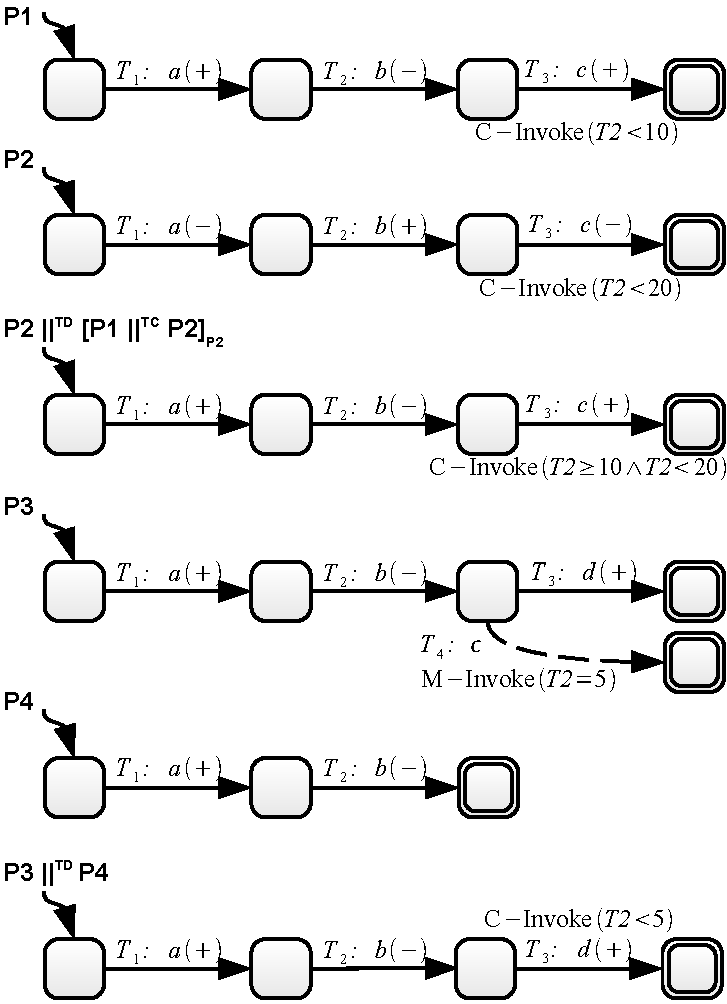
\includegraphics[width=0.8\textwidth]{content/protocol-analysis/compat-and-diff}
    \caption{Compatibility and replaceability analysis.}
    \label{fig:compat-and-diff}
\end{figure}

We give examples of operators-based compatibility and replaceability analysis on Figure~\ref{fig:compat-and-diff}. $\mathcal{P}_1$ and $\mathcal{P}_2$ are only partially compatible, as
$$ \projop{\mathcal{P}_1}{\mathcal{P}_2}{\mathcal{P}_2} \not\equiv \mathcal{P}_2 $$
By using the difference operator to compute $\mathcal{P}_2 \diffop \projop{\mathcal{P}_1}{\mathcal{P}_2}{\mathcal{P}_2}$, we get the set of conversations that are supported by $\mathcal{P}_2$ but not by $\mathcal{P}_1$ which yield to a partial compatibility ($\mathcal{P}_1$ does not support receiving a $c$ message after 10 units of time). $\mathcal{P}_4$ can be replaced by $\mathcal{P}_3$ as it supports all of the conversations that $\mathcal{P}_4$ supports: $\mathcal{P}_3 \sqsubseteq \mathcal{P}_4$. The converse is however not true as illustrated by $\mathcal{P}_3 \diffop \mathcal{P}_4$: $\mathcal{P}_3$ cannot handle $d$ messages.

% ........................................................................... %

\section{Discussion}

% ........................................................................... %

We briefly review the related work and discuss the limitations regarding the message-level matching that is performed in our approach.

% ........................................................................... %

\subsection{Related work}

% ........................................................................... %

\subsubsection{Verification techniques}

% ........................................................................... %

Many works in various fields have applied verification techniques such as checking for liveness, the absence of deadlocks or the conformance against specifications.
%
A substantial amount of work has been done in the field of workflow systems \cite{aalst98application,DMMZ06,BWJ02}.
In the case of web services, timed automata have been used in \cite{KazhamiakinPP06,DCPVC06}. In  \cite{berardi03finite} the introduced WSTL model had been designed with timing constraints as ``first-class citizen''. The analysis techniques presented in this paper did not leverage the timing constraints though, and while this had been mentioned as future work, it hasn't yet been done.\\

BPEL-based web services interactions have been analyzed in \cite{FBS04} by the mean of guarded automata with unbounded message queues where the automata synchronizablility problem is studied in synchronous and asynchronous communications.
Formal verification of service compositions is the target of several works: \cite{RouachedPG06,Bultan03,GLTXH07,FUMK03}.
The same types of verifications can be performed on protocol timed automata using TCTL, an extension of temporal logics for timed automata, and a model checker such as UPPAAL \cite{UPPAAL}.

% ........................................................................... %

\subsubsection{Compatibility and replaceability}

% ........................................................................... %

Software components have some fundamental similarities with web services: they promote good practices such as loose coupling and reuse. Also, they can be remotely accessed over a network. Similar approaches for protocols compatibility and replace-ability exist in the area of component-based systems \cite{Yellin97,CCLF+06}.\\

The importance of being able to check for services compatibility or replace-ability has lead to several research works \cite{MPC-TES01,FUMK-OE05,DBACTH05}. Surprisingly, these approaches do not cater for timing constraints.\\

They also perform ``black or white'' analysis. By contrast, our approach is able to provide a more fine-grained type of analysis by identifying the ``partial cases'' like the partial compatibility or the replace-ability with respect to a client protocol. We believe that this flexibility will significantly prove to be useful in practice, as full compatibility or replace-ability of business protocols can hardly be reached on the Internet which is an open service deployment environment.\\

The notion of process inheritance has been studied in the domain of workflows \cite{aalst03inheritance,Bussler02}. It is similar to protocols replaceability. Different types of inheritance relations are proposed in \cite{aalst03inheritance}. They provide some flexibility much like we did with the different classes of protocol replaceability. However, these approaches do not consider temporal abstractions.

% ........................................................................... %

\subsubsection{Model management}

% ........................................................................... %

The work that has been done in the model management area focuses on manipulating models (e.g., database schemas, XML schemas) and matches between them (e.g., equivalence between 2 database schema) on an equal foot \cite{BMPQ-SGR04}. The matches relationships between 2 models can be used for matching, merging or composition purposes. The models can also be manipulated through various operators like the intersection, the union or the difference.\\

A set of combined static and behavioral matching and merging techniques for statecharts-based specifications have been proposed in \cite{NSEZ-ICSE07}. This work has been done in a similar fashion as the approaches for schema matching (including databases and XML) mentioned in \cite{ERPB-VLDBJ01,BMPQ-SGR04}.\\

The work presented in this thesis shares some analogies with what has been done in this research field. Indeed, timed protocol is a model for which there exist protocol manipulation operators (composition, difference and intersection) as well as comparison operators (subsumption and equivalence).

% ........................................................................... %

\subsection{Message matching}

Our approach is mainly ``syntactic'' in the sense that when considering two messages named $\mathtt{login}$, we assume that both their schema and semantics are identical. This is of course not always the case in reality. As far as the schema is concerned, a better way for comparing two messages in the protocol operators would be to also look at their definitions (e.g., in XML Schema, grabbed from the services WSDL specifications). To do that, we could reuse schema matching algorithms as studied in \cite{ERPB-VLDBJ01,BMPQ-SGR04} or the approach presented in \cite{DongHMNZ04} which is more specific to web services interfaces. In some cases an adapter could be generated at the static interface level (messages schema and operations). \\

Another limit of the way that the messages matching is performed is that 2 messages $\mathtt{login}$ and $\mathtt{logUserIn}$ are considered to be different, although they could have exactly the same schema and/or semantics (or both could be ``close'' enough for easy adaptation). A potential solution would be to integrate the \emph{match} operator presented in \cite{NSEZ-ICSE07} with our compatibility and replaceability analysis techniques as it addresses such type of issues. The operator uses a heuristic that requires human intervention for identifying missing and invalid matches. If such an approach turned out to be useful, the identified message matches and mismatches could then be exploited to generate protocol adapters \cite{BenatallahCGNT05,MBMCC-WWW07}.

% ........................................................................... %

\chapter{Properties of protocol operators}
\label{chap:protocol-operators}
% ........................................................................... %

In the previous chapters, we have both introduced the model of \emph{timed protocols} and presented our approach for analyzing the pairwise compatibility or replaceability of two timed protocol instances. The set of flexible protocol compatibility and replaceability analysis classes that we presented can each be characterized by combining timed protocol operators. Yet, the decidability and closure properties of those operators remain to be studied ($\intersop$, $\compop$, $\diffop$, $\sqsubseteq$ and $\equiv$). To do that, we study those issues on protocol timed automata by reusing and adapting existing work from the theory of timed automata. As we will see, the case of $\intersop$ and $\compop$ is easy while the remaining operators pose more challenges. Indeed, they all rely on the ability to complement protocol timed automata, which is difficult as they have $\varepsilon$-labeled switches that cannot be removed in the general case. One strong theoretical contribution of this work is given here through the closure under complementation of protocol timed automata. This is the first class of timed automata with $\varepsilon$-labeled switches where this is possible.\\

This chapter is divided in two sections. The first one works at the protocol timed automata level and studies the closure of this class under intersection, then complementation. The second section leverages the results on protocol timed automata and translates them to timed protocols, leading to the decidability and closure properties of the timed protocol operators $\intersop$, $\compop$, $\diffop$, $\sqsubseteq$ and $\equiv$.

% ........................................................................... %

\section{Results in protocol timed automata}

% ........................................................................... %

We first study the intersection of protocol timed automata, then complementation. For each operator, the structure of the sections is identical: we give a procedure, an example and a theorem for the closure under the considered operator.

% ........................................................................... %

\subsection{Intersection of protocol timed automata}

% ........................................................................... %

The protocol timed automata intersection procedure extends the classical construction on timed automata \cite{RADLD94}, which in turns already extends the construction on (untimed) automata \cite{Hopcroft79}. We start by giving the procedure followed by an example. Then, we introduce a theorem for the closure of protocol timed automata under intersection.

\begin{procedure}
Given two protocol timed automata $A_1 = (L_1, L^0_1, L^f_1, X_1 \cup Y_1, E_1, \Sigma_1)$ and $A_2 = (L_2, L^0_2, L^f_2, X_2 \cup Y_2, E_2, \Sigma_2)$, the intersection $A_3 = A_1 \cap A_2$ (with $A_3 = (L_3, L^0_3, L^f_3, X_3 \cup Y_3, E_3, \Sigma_3)$) is built through the following steps.
\begin{enumerate}
  
  \item The locations are $L_3 = L_1 \times L_2$, the initial location is $L_3^0 = (L^0_1, L^0_2)$ and the final locations are $L_3^f = \left\lbrace (l_1, l_2) \;|\; l_1 \in L^f_1,\; l_2 \in L^f_2 \right\rbrace$.
  
  \item Two switches $e_1 = (l_1, g_1, a_1, r_1, l_1') \in A_1$ and $e_2 = (l_2, g_2, a_2, r_2, l_2') \in A_2$ are synchronized if and only if $a_1 = a_2 \neq \varepsilon$, producing a new switch $e_1e_2$ which is added to $A_3$: $e_1e_2 = ((l_1, l_2), g_1 \wedge g_2, a_1, \{x_{e_1e_2}\}, (l_1', l_2'))$ (this introduces a new clock $x_{e_1e_2}$ in $A_3$).
  
  \item $\varepsilon$-labeled switches are first added to $A_3$ with their guard being freed of $\permits$ clauses.
  We consider their guards to be disjunction-free (i.e., a $\varepsilon$-labeled witch whose guard is disjunctive is equivalent to several $\varepsilon$-labeled switches with conjunctive guards). 
  For each pair of $\varepsilon$-labeled switches
  $$
  \left\lbrace \begin{array}{l}
  
  e_1 = (l_1, (x_1 = k_1) \wedge g_1, \varepsilon, r_1, l_1') \in A_1 \\
  
  e_2 = (l_2, (x_2 = k_2) \wedge g_2, \varepsilon, r_2, l_2') \in A_2 \\
  
  \end{array} \right.
  $$
  we add the following switches to $E_3$:
  $$
  \left\lbrace \begin{array}{l}
  
  e_1e_\varepsilon = \left( (l_1, l_2), (x_1 = k_1) \wedge g_1 \wedge ((x_2 \neq k_2) \vee \neg g_2), \varepsilon, \{ x_{e_1e_\varepsilon} \}, (l_1', l_2) \right) \\
  
  e_\varepsilon e_2 = \left( (l_1, l_2), (x_2 = k_2) \wedge g_2 \wedge ((x_1 \neq k_1) \vee \neg g_1), \varepsilon, \{ x_{e_\varepsilon e_2} \}, (l_1, l_2') \right) \\
  
  e_1e_2 = \left( (l_1, l_2), (x_1 = k_1) \wedge (x_2 = k_2) \wedge g_1 \wedge g_2 , \varepsilon, \{ x_{e_1e_2} \}, (l_1', l_2') \right) \\
  
  \end{array} \right.
  $$
  
  \item With the set of clocks in $A_3$ being $X \cup Y$ as per definition, make sure that for each location $l$ offering at least one $\varepsilon$-labeled switch, a clock $y_l \in Y$ is reset on all of the incoming switches to $l$.
  
  \item For each location $l \in A_3$, compute the $\permits$ clauses.
  
  \item The guards in $A_3$ need to be rewritten to refer to the clocks of the switches of $A_3$ as they still refere to those of $A_1$ and $A_2$ at this step. A map is maintained between each clock $x_{e}$ of $A_1$ or $A_2$ and the set of clocks $\{ x_{e,e1}, x_{e,e2}, x_{e3,e}, \cdots \}$ that correspond to the switches $\{ (e,e1), (e, e2), \cdots, \}$ that were generated from $e$. Given a guard $g$ of a switch in $A_3$, a clause $(x_e \;\#\; k)$ of $g$ is rewritten as a disjunction $(x_{e,e1} \;\#\; k) \vee (x_{e,e2} \;\#\; k) \vee \cdots$. Diagonal constraint clauses in $g$ are also rewritten in a similar fashion using the mappings of its two clocks.
  
\end{enumerate}
\end{procedure}

\begin{figure}[htbp]
  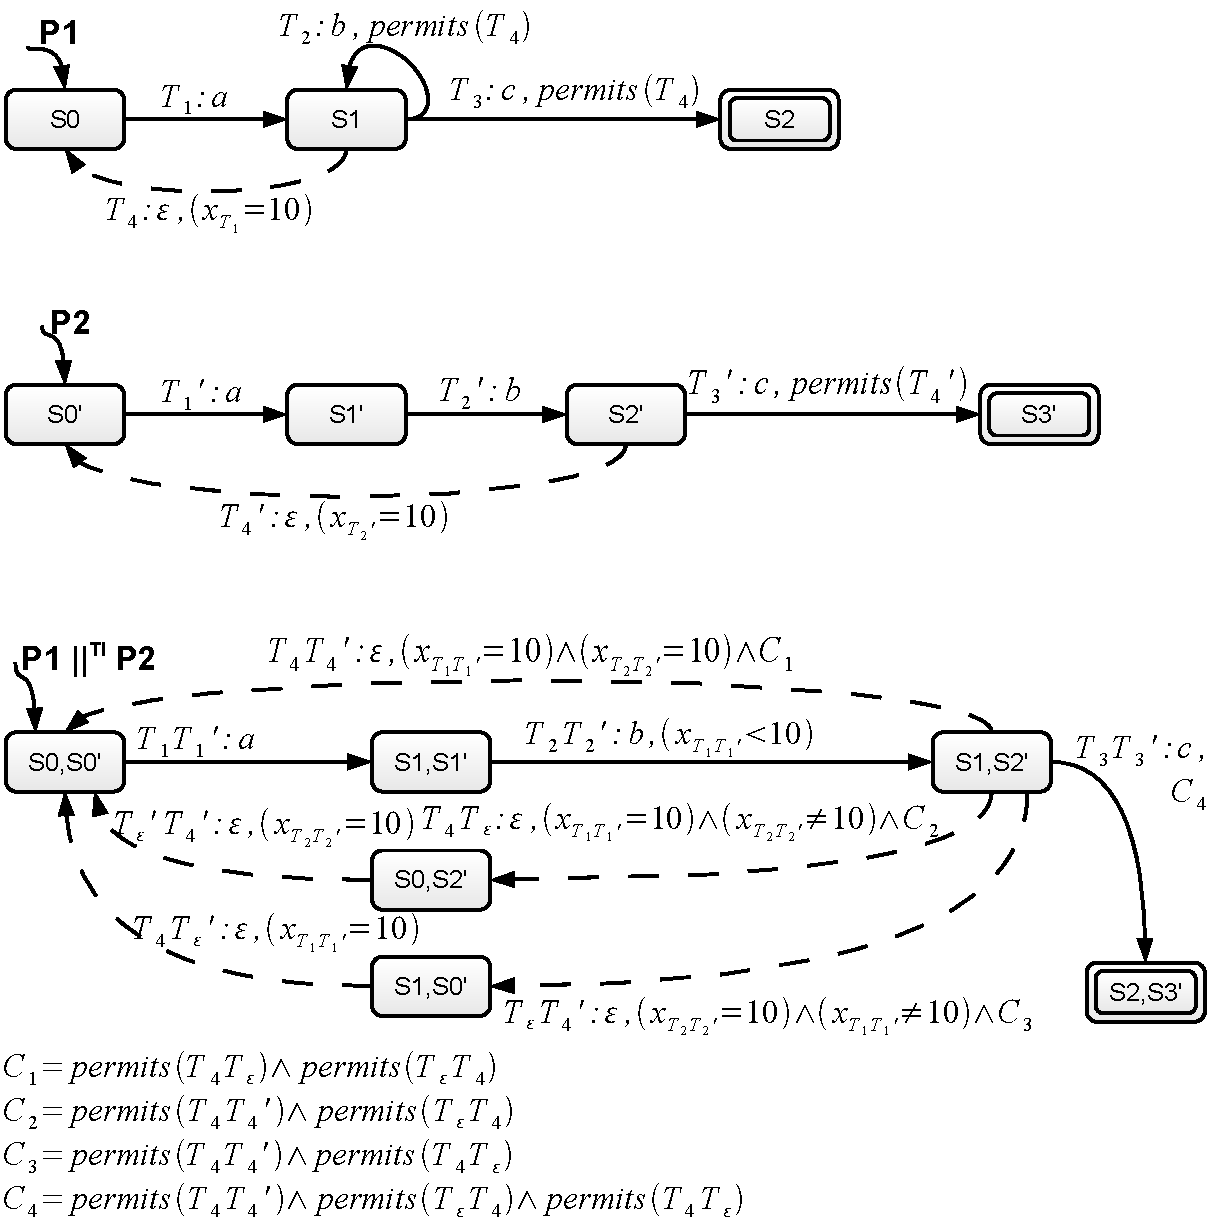
\includegraphics[width=\textwidth]{content/protocol-operators/sample-intersection}
  \caption{Two protocol timed automata $P_1$ and $P_2$ as well as their intersection $P_1 \intersop P_2$.}
  \label{fig:sample-intersection}
\end{figure}

Figure~\ref{fig:sample-intersection} gives an example of two protocol timed automata $P_1$ and $P_2$ as well as their intersection $P_1 \intersop P_2$. We deliberately abused notation for the sake of clarity by referring to transition identifiers in the $\permits$ functions instead of referring to guards.\\

Please note that in this procedure we remove the existing $\permits$ clauses in the guards as new ones are computed.
An extra step when actually implementing this procedure in a programming language would be to prune the locations that are not reachable from the initial location and the \emph{``deadlock''} locations, i.e., the non-final locations $l$ such that they don't provide any outgoing switch. The guards rewriting step is necessary because a switch of one of the input protocol timed automata may yield more than one switch in the resulting one. An example is the $T_4$ switch on $P_1$ from Figure~\ref{fig:sample-intersection} as it generates $T_4T_4'$, $T_4T_\varepsilon$, $T_\varepsilon T_4'$, $T_4T_\varepsilon'$ and $T_\varepsilon' T_4'$ in $P_1 \intersop P_2$. \\

Compared to the classic timed automata intersection procedure, the protocol timed automata intersection has the following differences.
\begin{enumerate}
  
  \item Clocks assignment remains ``under control'' to match the protocol timed automata requirement of having at most two clocks reset per transition. The classical timed automata intersection construction would simply combine the set of clocks from both input timed automata and merge the clocks in the reset sets of each switch. For example on Figure~\ref{fig:sample-intersection}, $T_2T_2'$ would reset the clock assigned to $T_2$ and the one assigned to $T_2'$.
  
  \item \MInvoke semantics are enforced in the intersection by computing new $\permits$ clauses (the $\permits$ clauses of the input timed automata guards are discarded).
  
\end{enumerate}

Protocol timed automata are closed under intersection (e.g., $A_3 = A_1 \cap A_2$ still belongs to the class).

\begin{theorem}
The class of protocol timed automata is closed under intersection.
\label{thm:closure-intersection}
\end{theorem}

The proof of the previous theorem is given on page~\pageref{proof:closure-intersection}.

% ........................................................................... %

\subsection{Complementation of protocol timed automata}

% ........................................................................... %

While protocol timed automata intersection is useful for characterizing timed protocol intersection and parallel composition, the complementation plays a critical role when it comes to characterizing the protocol difference and subsumption operators. Moreover, complementation of timed automata has traditionally been a difficult problem. Indeed, few classes of timed automata are closed under complementation \cite{RAPM04}.\\

We compute the complement of a protocol timed automaton using the following procedure which is derived from the one for deterministic timed automata as given in \cite{RADLD94}, with the difference lying in the presence of $\varepsilon$-transitions.

\begin{procedure}
Given a protocol timed automaton $A$, we denote by $A^*$ its \emph{complete} automaton which is build as follows.
\begin{enumerate}

  \item A location $q$ is added to $A^*$ whose role is to act as a \emph{rejection} location: given any timed word $w$ defined over $\overline{\mathcal{L}(A)}$, the execution of $w$ over $A^*$ goes to the location $q$ as soon as an input symbol yields to a word which is not in $\mathcal{L}(A)$. Hence, any timed word $w$ defined over the alphabet of $A$ has a (unique) execution over $A^*$.

  \item For each location $l$ of $A$ (this includes $q$) and for each word $a$ of the alphabet, a transition
  $$ 
  e = \left( 
    l, \left( g \bigwedge\limits_{1 \leq i \leq n} \permits(g_{\varepsilon i}) \right), a, \{ x_e \}, q
    \right)
  $$ is added where:
  \begin{enumerate}
    \item $g$ is defined as the negation of the disjunctions\footnote{e.g., given 2 $a$-labeled switches with guards $g_1$ and $g_2$, $g = \neg(g_1 \vee g_2)$} of the guards\footnote{For each guard, we do not take into account the clauses that are obtained through the $\permits$ function.} of the other $a$-labeled transitions from $l$, and
    \item each $g_{\varepsilon i} = (x_i = k_i) \wedge g_{\varepsilon i}'$ appears in the guard of the $i$-th $\varepsilon$-labeled switch from $l$, given that $l$ offers $n \geq 0$ of such switches.
  \end{enumerate}

\end{enumerate}
As in \cite{RADLD94}, the complement $\overline{A}$ of $A$ is deduced from $A^*$ by inverting the final and the normal locations due to the fact that every timed word $w \in \mathcal{L}(A)$ has a unique run over $A$.
\end{procedure}

\begin{figure}[htbp]
  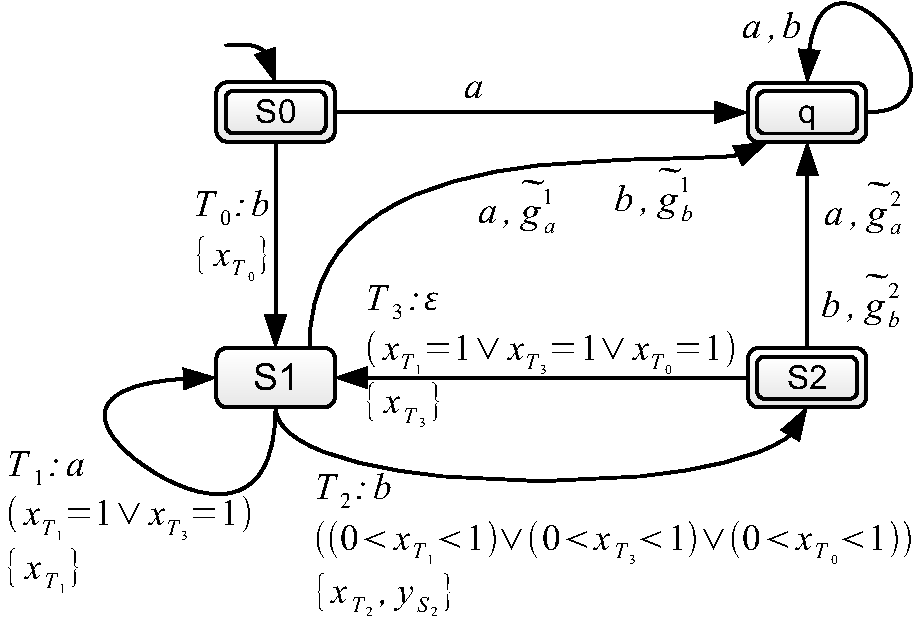
\includegraphics[width=\textwidth]{content/protocol-operators/complement-precise-time}
  \caption{The complement of the protocol timed automaton of Figure~\ref{fig:precise-time} (with drawing shortcuts).}
  \label{fig:complement-precise-time}
\end{figure}

As an example, we give on Figure~\ref{fig:complement-precise-time} the complement of the protocol timed automaton of Figure~\ref{fig:precise-time}. For the sake of clarity, we took some shortcuts in the drawing by combining the switches to $q$ that have been added from the same source location. The added guards are as follows:
\begin{itemize}
  
  \item $\widetilde{g_a^1} = (x_{T_1} \neq 1) \wedge (x_{T_3} \neq 1)$
  
  \item $\widetilde{g_b^1} = (x_{T_1} = 0 \vee x_{T_1} \geq 1) \wedge (x_{T_3} = 0 \vee x_{T_3} \geq 1) \wedge (x_{T_0} = 0 \vee x_{T_0} \geq 1)$
  
  \item $\widetilde{g_a^2} = \widetilde{g_b^2} = $
  
    $\left(
     (x_{T_1} < 1) \vee \left( (x_{T_1} > 1) \wedge (x_{T_1} - y_{S_2} > 1) \right)
    \right)
    \bigwedge$    
    
    $\left(
      (x_{T_3} < 1) \vee \left( (x_{T_3} > 1) \wedge (x_{T_3} - y_{S_2} > 1) \right)
    \right)    
    \bigwedge$
    
    $\left(
      (x_{T_0} < 1) \vee \left( (x_{T_0} > 1) \wedge (x_{T_0} - y_{S_2} > 1) \right)
    \right)$
  
\end{itemize}

As mentioned in the next theorem (a proof is given on page~\pageref{proof:closure-complement}), protocol timed automata are closed under complementation. This is a very interesting result, not only because it allows us to properly implement a timed protocol operator such as the difference, but also because the introduction of $\varepsilon$-labeled switches strictly increases expressiveness over (indeterministic) timed automata. Interestingly, previous results would not have suggested that protocol timed automata would be closed under complementation.

\begin{theorem}
The class of protocol timed automata are closed under complementation.
\label{thm:closure-complement}
\end{theorem}

The proof is given on page~\pageref{proof:closure-complement}.

% ........................................................................... %

\section{Results for timed protocol operators}

% ........................................................................... %

The closure properties of protocol timed automata under intersection and complementation allows to derive the following theoretical results for timed protocol operators.
The result on the intersection and parallel composition operators is straightforward.

\begin{corollary}
Timed protocols are closed under $\intersop$, $\compop$ and $\diffop$.
\end{corollary}

Both $\intersop$ and $\compop$ operators are based on the intersection using a different matching of the messages depending on their polarities:
\begin{itemize}
  
  \item in the case of $\intersop$, two messages match when they have the same name and polarity (e.g., $a(+)$ and $a(+)$)
  
  \item in the case of $\compop$, two messages match when they have the same name but a different polarity (e.g., $a(+)$ and $a(-)$).
  
\end{itemize}

The result on the difference operator derives from the closure of protocol timed automata under both intersection and complementation. Indeed, $\mathcal{P}_1 \diffop \mathcal{P}_2$ is equivalent to $\mathcal{P}_1 \intersop \overline{\mathcal{P}_2}$, hence timed protocol are also closed under difference.

\begin{corollary}
The timed protocol comparison operators $\sqsubseteq$ and $\equiv$ are decidable.
\end{corollary}

This comes from the closure under complementation and intersection as well as from the decidability of the reachability problem \cite{RADLD94}. Checking if $L(A_1) \subseteq L(A_2)$ is equivalent to checking whether $L(A_1 \cap \overline{A_2}) = \emptyset$ or not. A technique for checking emptiness of protocol timed automata using the UPPAAL model checker is discussed in the appendix at page~\pageref{chap:uppaal-pta}.

% ........................................................................... %

% ........................................................................... %

% ........................................................................... %

\part{Applications and perspectives}

% ........................................................................... %

\chapter{The ServiceMosaic Protocols project}
\label{chap:protocols-project}
% ........................................................................... %

This chapter presents the implementation of the contributions contained in this thesis work. We first present \emph{ServiceMosaic}, the umbrella project in which this work has been made. We then focus on the components that we have implemented for modeling and analyzing timed business protocols.

% ........................................................................... %

\section{ServiceMosaic}

% ........................................................................... %

This section presents the ServiceMosaic project. We first give an outlook of the general project architecture, then provide some technical details regarding how the various projects that compose ServiceMosaic are made.

% ........................................................................... %

\subsection{Project overview}

% ........................................................................... %

ServiceMosaic\footnote{See \url{http://servicemosaic.isima.fr/}} is an international project for research in the context of web services. It currently acts as a bridge between several research groups:
\begin{itemize}

	\item the SOC Group at the University of New South Wales, Sydney, Australia
	
	\item the APIS Research Group at Universit\'e Blaise Pascal, Clermont-Ferrand, France
	
	\item the BD-RCR Group at Universit\'e Claude Bernard, Lyon, France
	
	\item the group of Fabio Casati at the University of Trento, Italy.

\end{itemize}

\begin{figure}[tbhp]
    \centering
    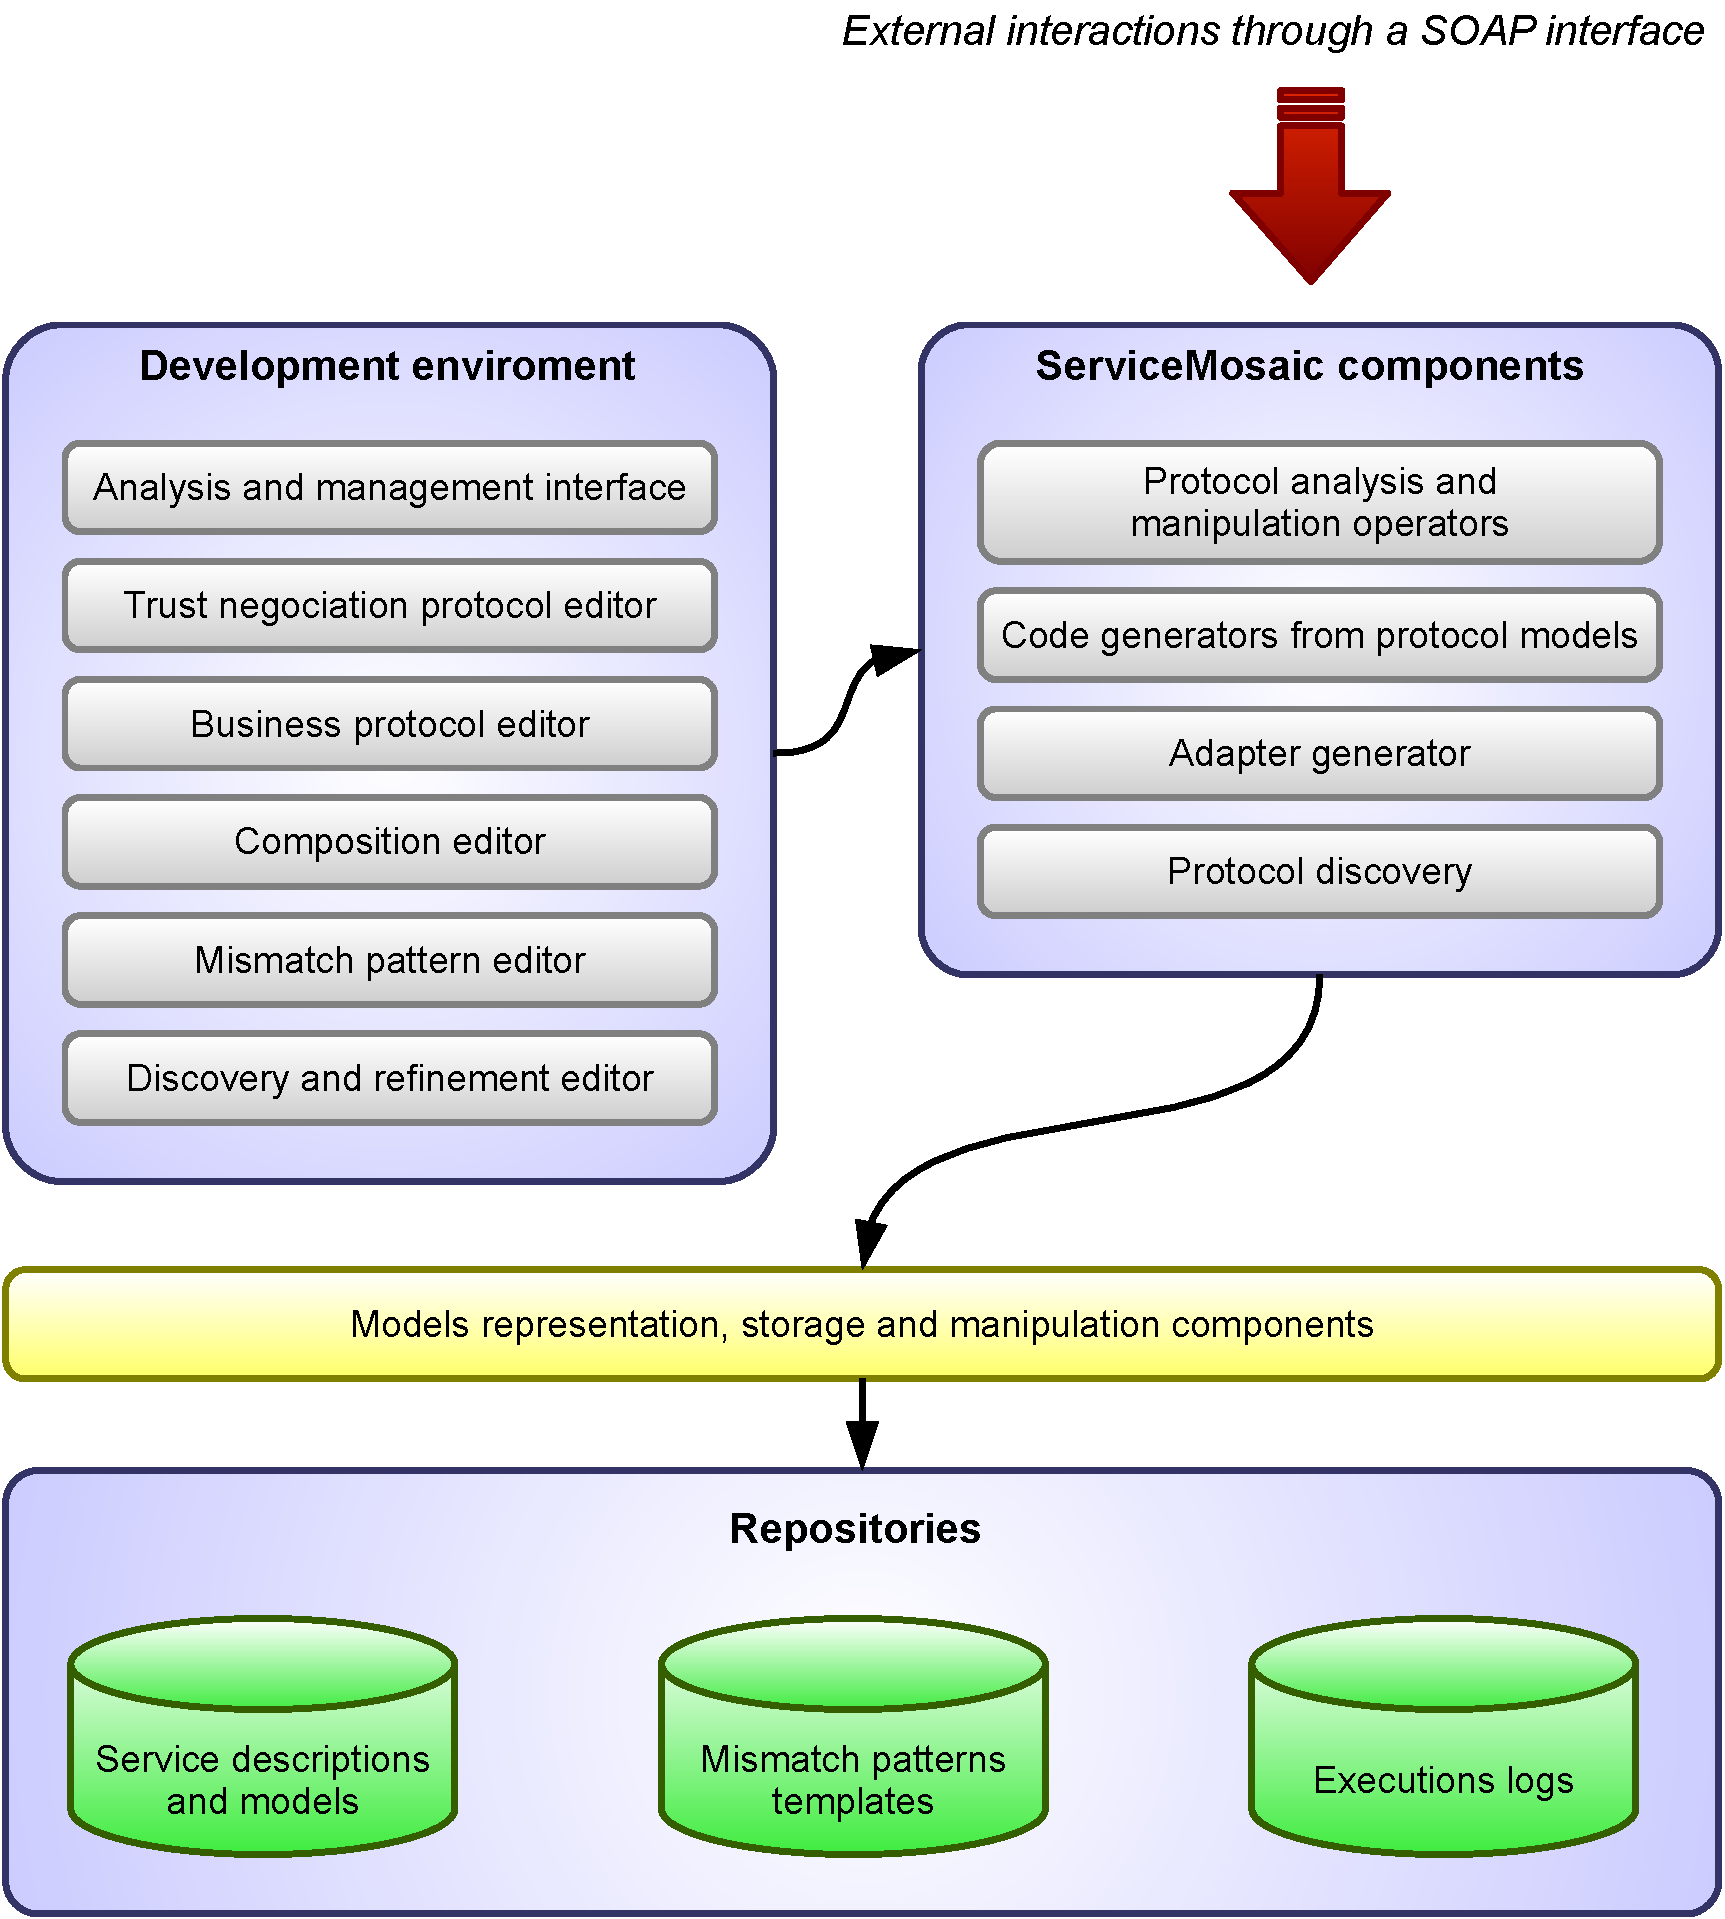
\includegraphics[width=\textwidth]{content/protocols-project/servicemosaic-architecture}
    \caption{Architecture overview of the ServiceMosaic platform.}
    \label{fig:servicemosaic-architecture}
\end{figure}

ServiceMosaic is a CASE platform for supporting the service development life-cycle that includes facilities for modeling, analyzing, discovering and adapting web service models \cite{BCTPM06-SM,NezhadSBCPT07}. The architecture, depicted on Figure~\ref{fig:servicemosaic-architecture}, comprises the following components.
\begin{description}
  
  \item[Models and manipulation components] support representing, storing an manipulating service descriptions and protocols. We provide basic manipulation operations of model elements such as protocols as core libraries that shield higher-level components from the details of their physical representations (e.g., plain files, XML, relational databases and so on).
  
  \item[Analysis and management components] include operators for protocol compatibility and replaceability analysis \cite{FTBB}, a code generator that produces BPEL skeletons from protocols \cite{BBFC04}, a code generator that produces BPEL templates for implementing the adapters \cite{BenatallahCGNT05,NezhadBMCC07}, and protocol discovery from service execution logs \cite{Motahari-NezhadSBC07}.
  
  \item[The development environment] provides visual exploration for modifying, analyzing and managing model elements. For example, it offers editors for business protocols, trust negotiation protocols \cite{SkogsrudBCD04,SkogsrudBC03} and orchestration models.
  
\end{description}

Finally, the ServiceMosaic components can be accessed through a set of programmatic SOAP web service interfaces. Each service is a simple thin wrapper on top of the components application programming interfaces.

% ........................................................................... %

\subsection{Technical overview}

% ........................................................................... %

The tools that we develop use the Java\tm platform version 5\footnote{See \url{http://java.sun.com/j2se/1.5.0/}}. Most developments are being made using the Java\tm programming language, but given the recent interest in dynamic languages that run on the Java\tm platform (e.g., Groovy, Ruby, Python, etc), we are allowing their use where useful. Indeed, the language facilities that are provided by some of those languages (e.g., functional programming inspired constructs such as closures\footnote{Martin Fowler gives a good concise presentation of closures at \url{http://martinfowler.com/bliki/Closure.html}}) allow for writing code that is arguably more concise and easier to read and maintain.\\

For every project, the development approach is the following:
\begin{enumerate}
  
  \item develop functionalities as standalone, reusable libraries that can be used in console, desktop, web or service-based tools, and
  
  \item expose the functionalities in development tools as plug-ins for the Eclipse platform\footnote{See \url{http://www.eclipse.org/}}.
  
\end{enumerate}

The choice of Eclipse as a development tools platform is justified by the following reasons. First of all, it is an open-source platform whose goal is to explicitly integrate tools from various vendors inside the same environment. As such, it provides several APIs and frameworks for building applications that can seamlessly integrate with third-party ones. The benefits for a research project are numerous.
\begin{enumerate}
  
  \item The implementation work can be focused on the sole contribution of each work, not on less critical details such as providing common dialog boxes, a preferences support framework, or integrated user assistance.
  
  \item The integration with new developments from inside the ServiceMosaic project or third-parties is vastly facilitated since a common foundation is being used. In most cases, the plug-ins that bring the contributions can simply be assembled inside an Eclipse-based environment without any modification having to be made.
  
  \item The Eclipse ecosystem is broad with a mixture of open-source and commercial offerings (see \url{http://www.eclipse.org/membership/exploreMembership.php}). As such, it is a positive factor for facilitating the dissemination of the work that we conduct.
  
\end{enumerate}

\begin{figure}[tbhp]
    \centering
    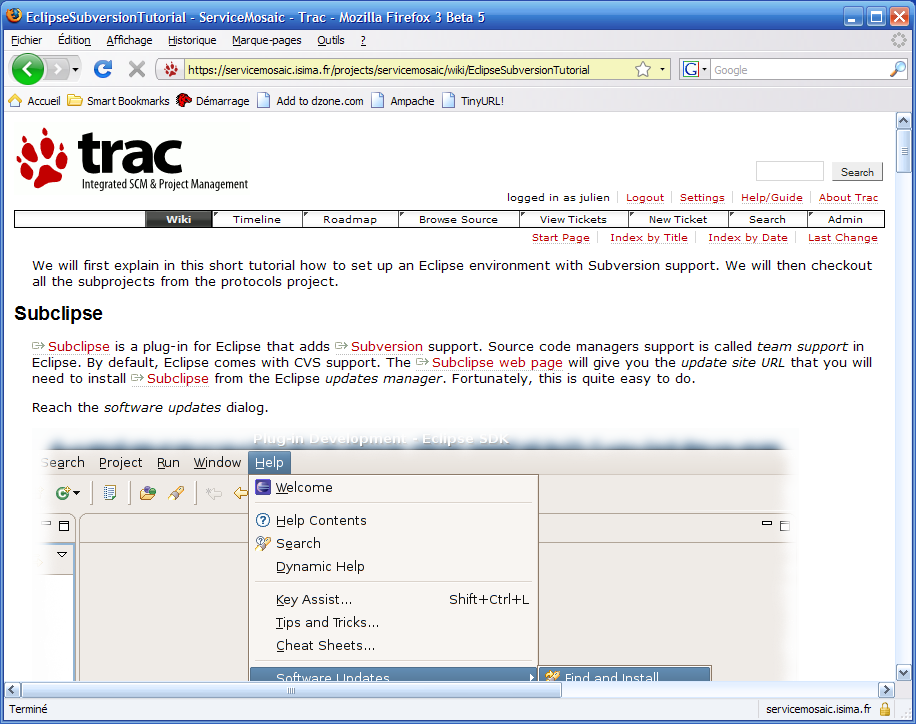
\includegraphics[width=\textwidth]{content/protocols-project/trac-wiki}
    \caption{Trac wiki view.}
    \label{fig:trac-wiki}
\end{figure}

\begin{figure}[tbhp]
    \centering
    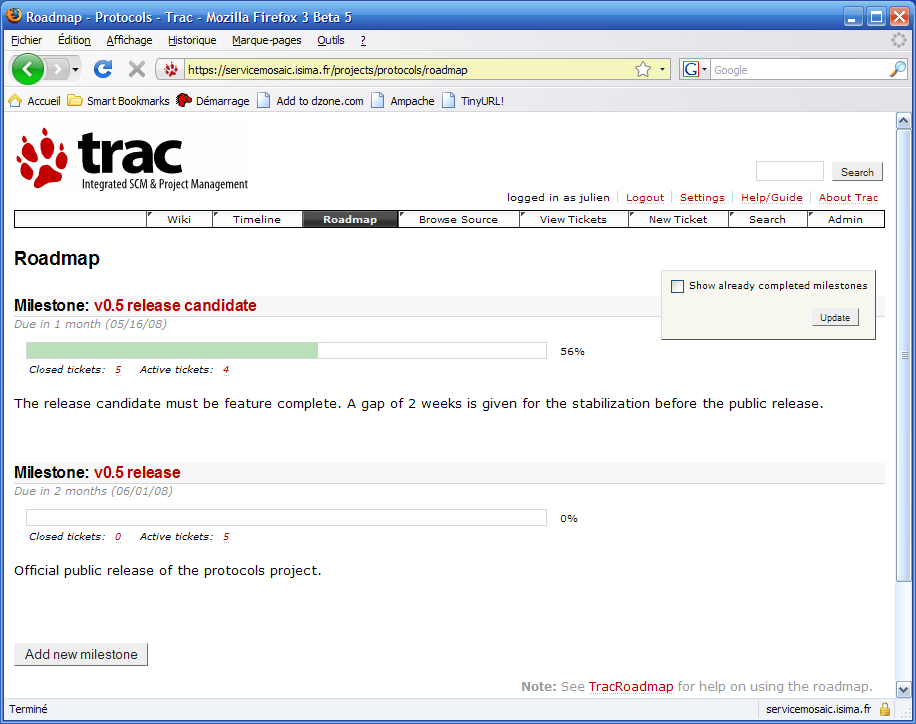
\includegraphics[width=\textwidth]{content/protocols-project/trac-roadmap}
    \caption{Trac roadmap view.}
    \label{fig:trac-roadmap}
\end{figure}

The platform being developed across different institutions around the world, we have deployed a server at \url{http://servicemosaic.isima.fr/} with collaborative services:
\begin{itemize}
  
  \item the source code management and versioning is done using Subversion (see \url{http://subversion.tigris.org/}), allowing for distributed, concurrent modifications and sharing of the source code bases
  
  \item each project has an instance of Trac (see \url{http://trac.edgewall.org/}), a web-based application for managing projects that offers a wiki (see Figure~\ref{fig:trac-wiki}), a source code browser (integrated with Subversion, see Figure~\ref{fig:trac-svn}), a roadmap (see Figure~\ref{fig:trac-roadmap}) and an issues manager (defects, tasks, enhancements, see Figure~\ref{fig:trac-issues}).
  
  \item mailing-lists and public / private download areas are available
  
  \item a JavaEE 5 compliant application server\footnote{In our case, we chose to run Glassfish from Sun Microsystems: \url{http://glassfish.org/}.} is available for the deployment of server-side applications, including web applications and web services.
  
\end{itemize}

\begin{figure}[tbhp]
    \centering
    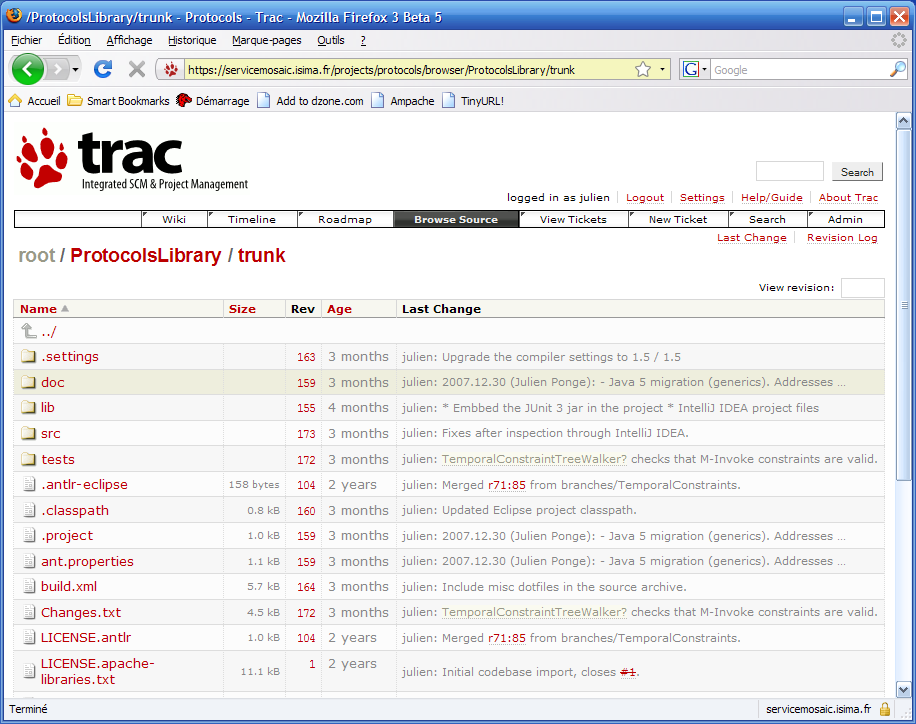
\includegraphics[width=\textwidth]{content/protocols-project/trac-svn}
    \caption{Trac source browser view.}
    \label{fig:trac-svn}
\end{figure}

\begin{figure}[tbhp]
    \centering
    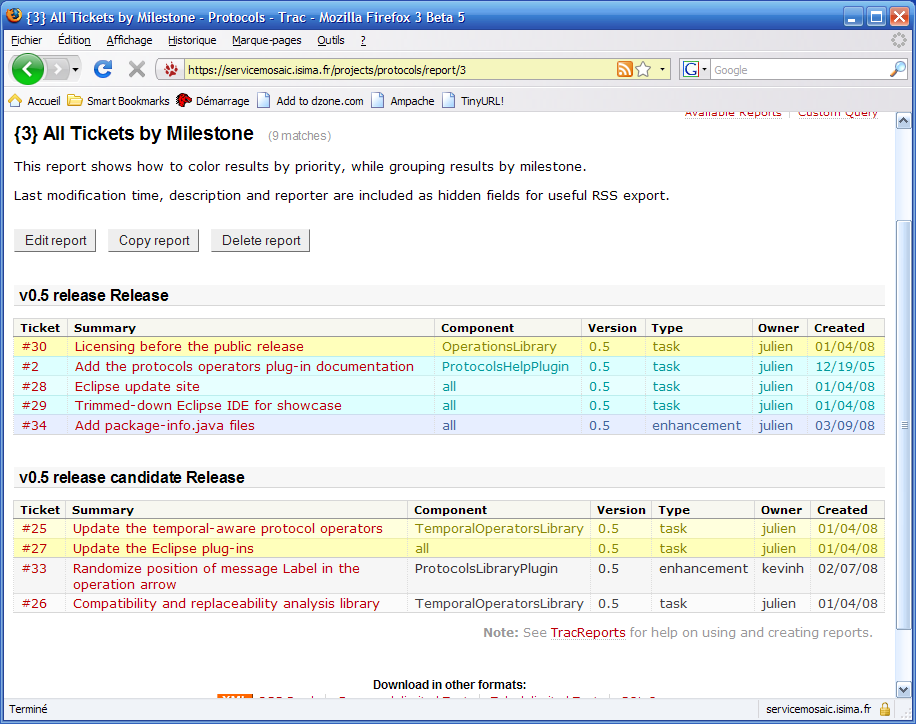
\includegraphics[width=\textwidth]{content/protocols-project/trac-issues}
    \caption{Trac issues management view.}
    \label{fig:trac-issues}
\end{figure}

A number of projects implemented as part of the ServiceMosaic platform are set to be progressively released to the public over time.

% ........................................................................... %

\section{Prototype: the ServiceMosaic Protocols project}

% ........................................................................... %

\begin{figure}[tbhp]
    \centering
    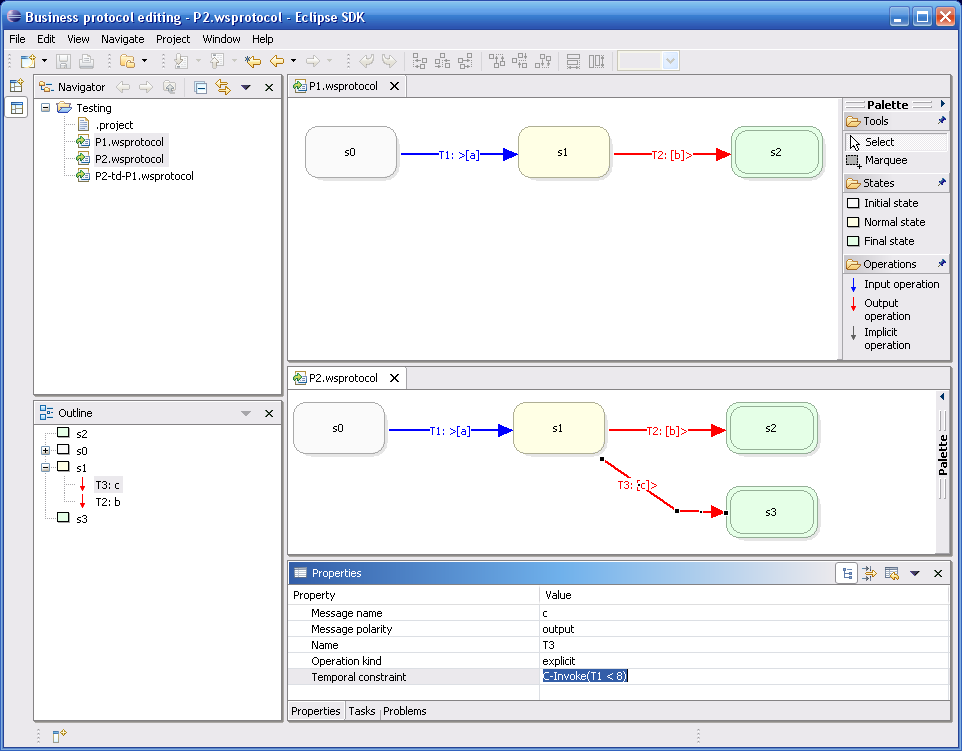
\includegraphics[width=\textwidth]{content/protocols-project/proto-screenshot}
    \caption{Screenshot of the ServiceMosaic Protocols prototype.}
    \label{fig:proto-screenshot}
\end{figure}

The work presented in this thesis has been implemented as part of a subproject of ServiceMosaic called \emph{ServiceMosaic Protocols}. It groups the libraries and development tools that are related to business protocol modeling, analysis and management. Figure~\ref{fig:proto-screenshot} shows a screenshot of the prototype development environment which is based on the Eclipse platform. It features two business protocol being edited, including timing constraints.

% ........................................................................... %

\subsection{Components}

% ........................................................................... %

\begin{figure}[tbhp]
    \centering
    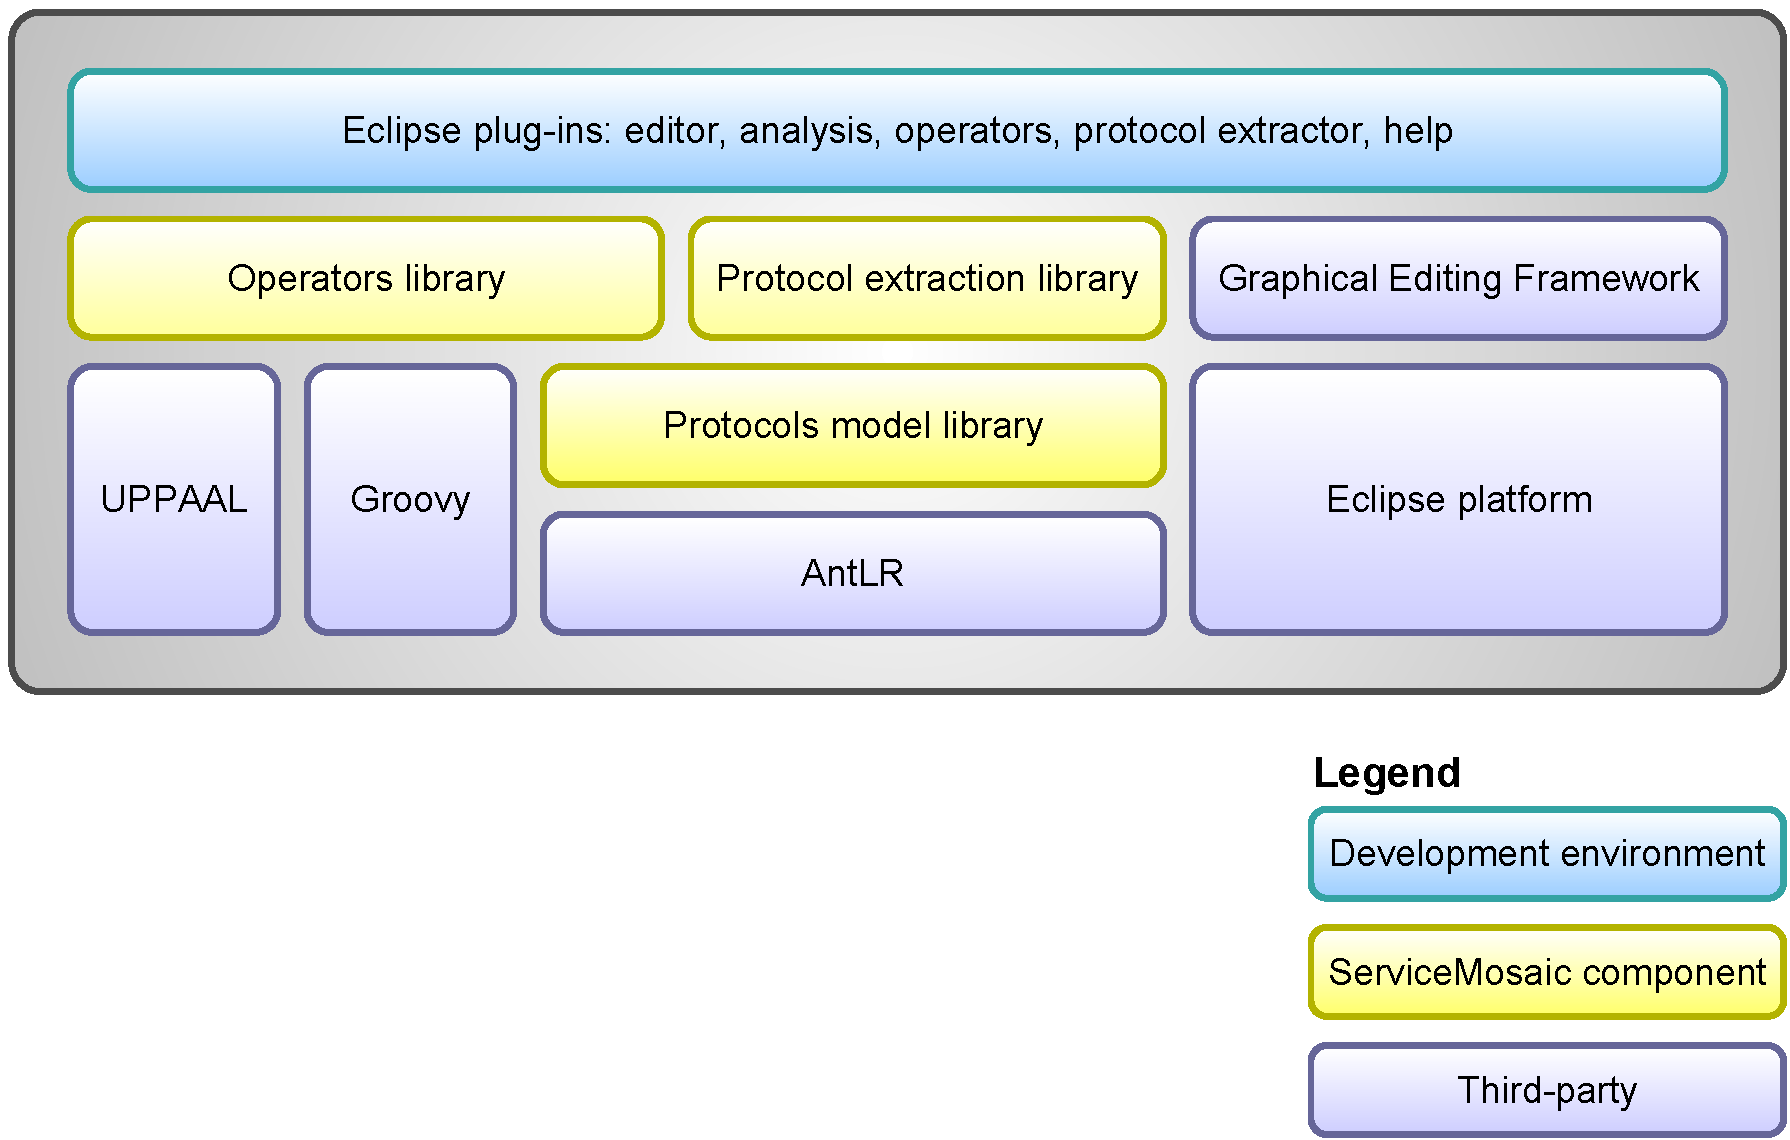
\includegraphics[width=\textwidth]{content/protocols-project/protocols-proto-layers}
    \caption{Architecture of the ServiceMosaic Protocols prototype.}
    \label{fig:protocols-proto-layers}
\end{figure}

The following components have been developed as part of the ServiceMosaic Protocols project, as depicted on Figure~\ref{fig:protocols-proto-layers}.
\begin{description}
  
  \item[A business protocols model library] has been developed. It contains an object-oriented model for representing and manipulating business protocols. While abstracting from the physical representation of protocols (e.g, files, databases, ...), it contains a simple XML persistence class that allows protocols to be stored and read from various XML sources (e.g., files, XML databases, network interface, ...). Temporal constraints are explicitly supported by the library. They are stored as plain strings in the model that are attached to the transitions of a protocol. However, a complete object model is part of the library for manipulating temporal constraints (e.g., programmatically constructing an in-memory constraint, computing the conjunction of two constraints, renaming variables, computing the negation of a constraint, ...). We use a parser written using AntLR\footnote{AntLR is actively developed at \url{http://www.antlr.org/}.} \cite{ParrQ95} for obtaining the object model that corresponds to a constraint in a plain string and vice-versa. As such, the protocol model library is self-contained.
  
  \item[A protocol manipulation and comparison operators library] has been developed using the Groovy language  \cite{Groovy07}. It implements the complete range of business protocol operators (i.e., $\intersop$, $\compop$, $\diffop$, $\sqsubseteq$, $\equiv$). The operators can be used ``as-is'', or a facade class can be used for directly assessing compatibility or replaceability between two protocols. In fact, the facade class does nothing but invokes the manipulation and comparison operators as described in Table~\ref{tab:classes-characterization}. Emptiness checking is required by some operators. It is done using the UPPAAL model checker using the technique that is presented from page~\pageref{chap:uppaal-pta}.
  
  \item[A set of Eclipse plug-ins] have been developed, based on the libraries mentioned above and the Eclipse platform. The business protocol editor is based on a set of customized SWT/JFace figures (e.g., the shape of states in a protocol) and the Eclipse Graphical Editing Framework (see \url{http://www.eclipse.org/gef/}). It can take advantage of WSDL documents for ensuring that only valid messages are being put into protocols by designers. The analysis components provide a visual interface for either invoking the manipulation and comparison operators, or directly checking for compatibility and replaceabilty of protocols. An embedded help support is available for providing assistance.
  
\end{description}

The figure also depicts a \emph{protocol extraction} component. This companion component having been developed by an engineering intern of the APIS Research Group\footnote{See \url{http://apis.isima.fr/}.}, and since it is still very experimental at this stage, it will be presented separately in the following section.\\

To make the libraries easier to use, we adopted the use of \emph{fluent interfaces} \cite{FowlerFI05}. Briefly, such ``fluent'' interfaces tend to use techniques such as making method calls chainable. This arguably makes the code sometimes easier to read, and in many cases, fluent interfaces can be enough for making an \emph{internal domain-specific language} \cite{FreemanP06,FowlerDSL04}. \\

The components developed in this project have served as the basis of many other ServiceMosaic projects. For example, the protocols model library serves as the standard ServiceMosaic library for developing components that manipulate protocols. Also, the protocol editor has been used in derivative works such as the protocol discovery and refinement tool \cite{Motahari-NezhadSBC07}.\\

The ServiceMosaic Protocols project are staged to be released in 2008 under the terms of the \emph{GNU Lesser General Public License version 3}\footnote{See \url{http://www.gnu.org/licenses/lgpl.html}.}, a moderate open-source license that facilitates dissemination of the work while enforcing modifications of the code to be released under the same licensing conditions.

% ........................................................................... %

\subsection{Protocol extraction}

% ........................................................................... %

We now outline a \emph{protocol extraction operator}, developed externally as part of the ServiceMosaic project, that takes a BPEL process as input and outputs a \emph{multi-party protocol}, which is basically an extension of a timed protocol where a message is also tagged with the \emph{partner link} of the service which is sending or receiving the message.
Hence, a multi-party business protocol captures the global message \emph{choreography} of a BPEL process.\\

To extract the multi-party protocol we proceed as follows.
First, we identify \emph{protocol extraction patterns} for each type of  basic and complex BPEL activity. The extraction starts from the beginning of the process and goes through each activity to apply the protocol extraction patterns as such they are recognized. When a complex activity is encountered (e.g., \emph{if}, \emph{switch}, \emph{while}, \emph{pick}, ...), it is recursively processed on each of its complex activities until basic activities are reached. Hence, the obtained protocol fragments are assembled by inverse recursion. For instance, if a \emph{if} activity comprises one \emph{invoke} on each alternative branch, then a protocol fragment is derived from each \emph{invoke}, then they are combined as different branches from the current state in the extraction process.\\

\begin{figure}[tbhp]
    \centering
    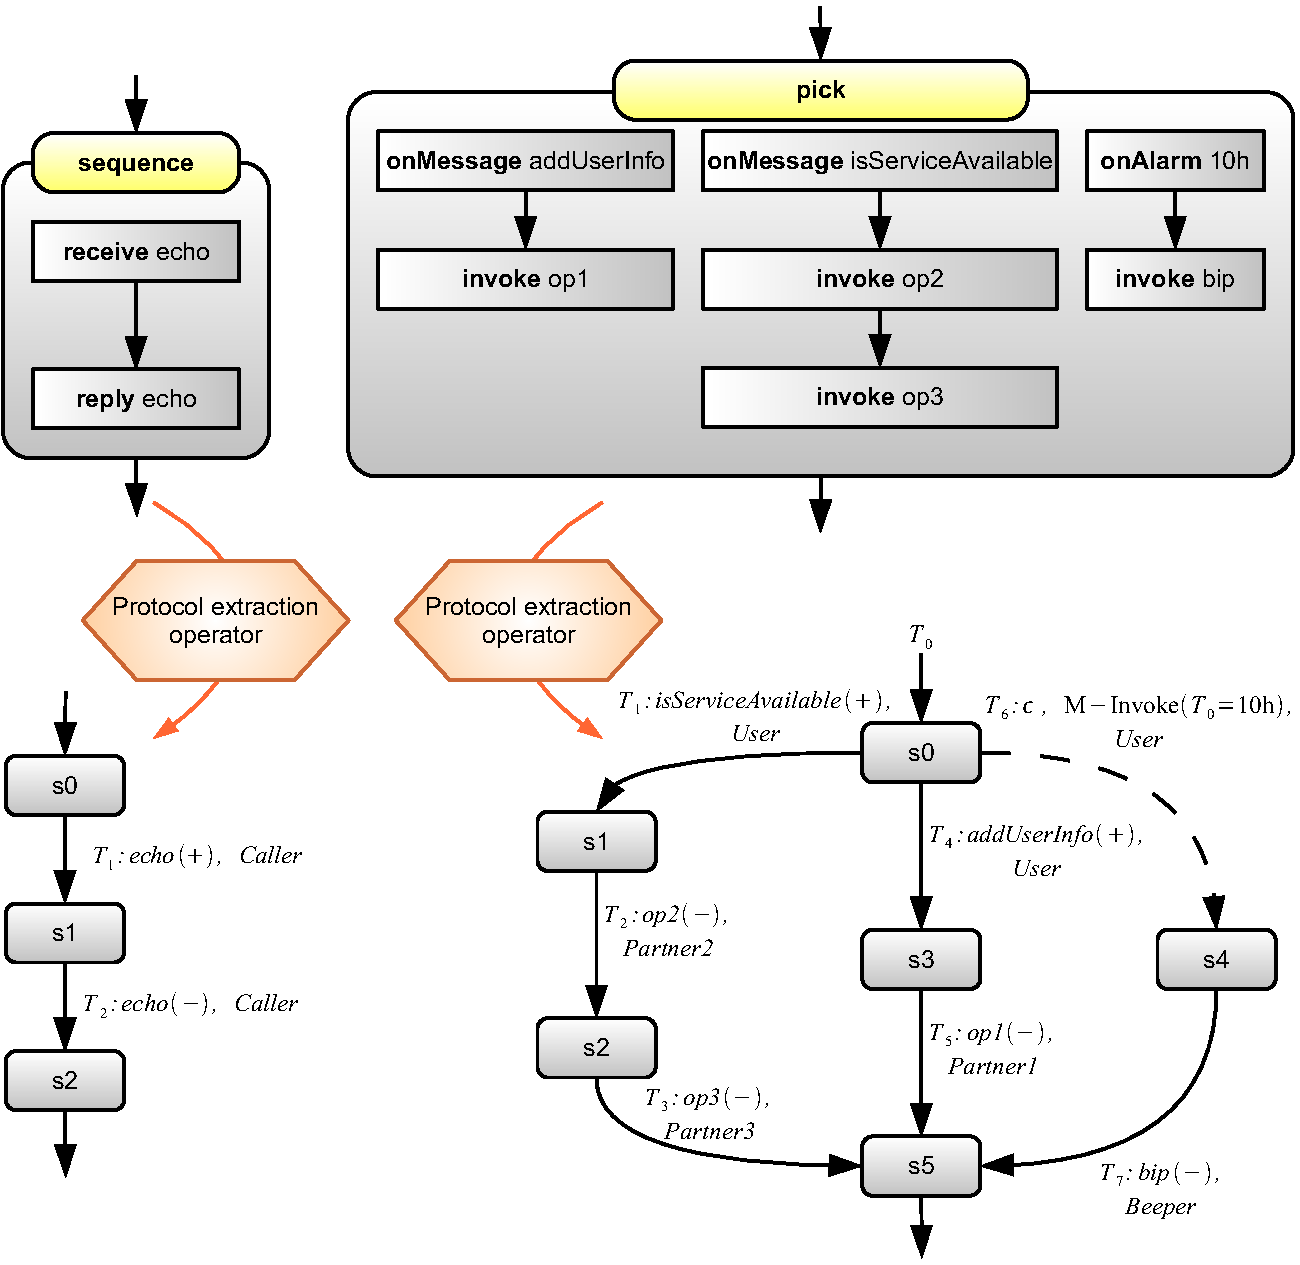
\includegraphics[width=\textwidth]{content/protocols-project/bpel2protocol}
    \caption{Extraction of multi-party protocols fragments from BPEL.}
    \label{fig:bpel2protocol}
\end{figure}

We give two examples of BPEL patterns extractions on Figure~\ref{fig:bpel2protocol}. The first example shows a simple \emph{sequence} activity that consists of a \emph{receive} activity followed by a \emph{reply}. What is done by the sequence is simply the echo-ing of a message. This is translated using two transitions (one for each message). Because a multi-party protocol is extracted, each transition is also tagged with the partner link (e.g. \emph{Caller}) and the BPEL activity (e.g. \emph{reply}).\\

The second example shows a \emph{pick} complex activity involving two message handlers and an alarm handler. Each message or alarm handler leads to a branch for the message choreography that corresponds to its activities. For example on the \emph{addUserInfo} message handler, there is a $op1$ invocation on the \emph{Partner1} partner link. The \emph{onAlarm} handler leads to an implicit transition featuring a \MInvoke constraint. Temporal informations can be extracted from either \emph{onAlarm} handlers or \emph{wait} activities. Finally, all branches join in the state $s_5$ which corresponds to the end of the \emph{pick} activity.\\

Note that this transformation is not reversible. When generating a protocol, we only care about possible ordering of messages and not about the many details prescribed by a BPEL process (such as why -- based on which condition -- a certain path is chosen). Nevertheless, we had developed developed techniques for generating service implementation templates in BPEL from protocols definitions \cite{KBBB+04}.\\

The protocol which is followed by the process while interacting with a given service (identified by its BPEL \emph{partner link}) can be obtained as follows. The idea is to perform a special form of filtering on the multi-party protocol. In a similar fashion as \emph{projection} for timed automata \cite{RAPM04}, we replace the messages with $\varepsilon$ on the transitions that are not associated with the partner link of the service that we are interested in. Also, each temporal constraint that refers to a transition which is not from the target partner link is removed. Indeed, they do not make sense in the protocol that we want to obtain since they refer to events that are not ``seen'' by the orchestrated service. Finally, the service protocol is obtained by removing the $\varepsilon$ transitions using standard techniques on automata \cite{Hopcroft79}. This is possible only because if we mapped to timed automata, there would be no guard nor clock resets on these transitions \cite{VDPG97}.\\

In our experiments, we have found out that the protocol extraction operator works well for a large majority of BPEL processes. As mentioned previously, this protocol extraction operator is absolutely not part of this thesis work contributions. It will require further investigations, including formalization, a proper theoretical study and implementation work.

% ........................................................................... %


\chapter{Protocol analysis at work}
\label{chap:sample-usecase}
% ........................................................................... %

We now show how the prototype and protocol analysis approach can be used to facilitate service development on the following scenario. The scope of applications of protocol analysis goes however beyond just this example as we will see in the next chapter.
%
We assume here that a developer is defining a BPEL process, related to the handling of a purchase order, and that the process invokes several services during its execution. The tool will assist the developer in checking if the selected services have a protocol which is fully or partially compatible with the defined BPEL process, will identify which conversations can and cannot be carried out, and will also tackle the case of non compatibility by supporting the development of protocol adapters.

% ........................................................................... %

\section{BPEL process outline}

% ........................................................................... %

\begin{figure}[tbhp]
    \centering
    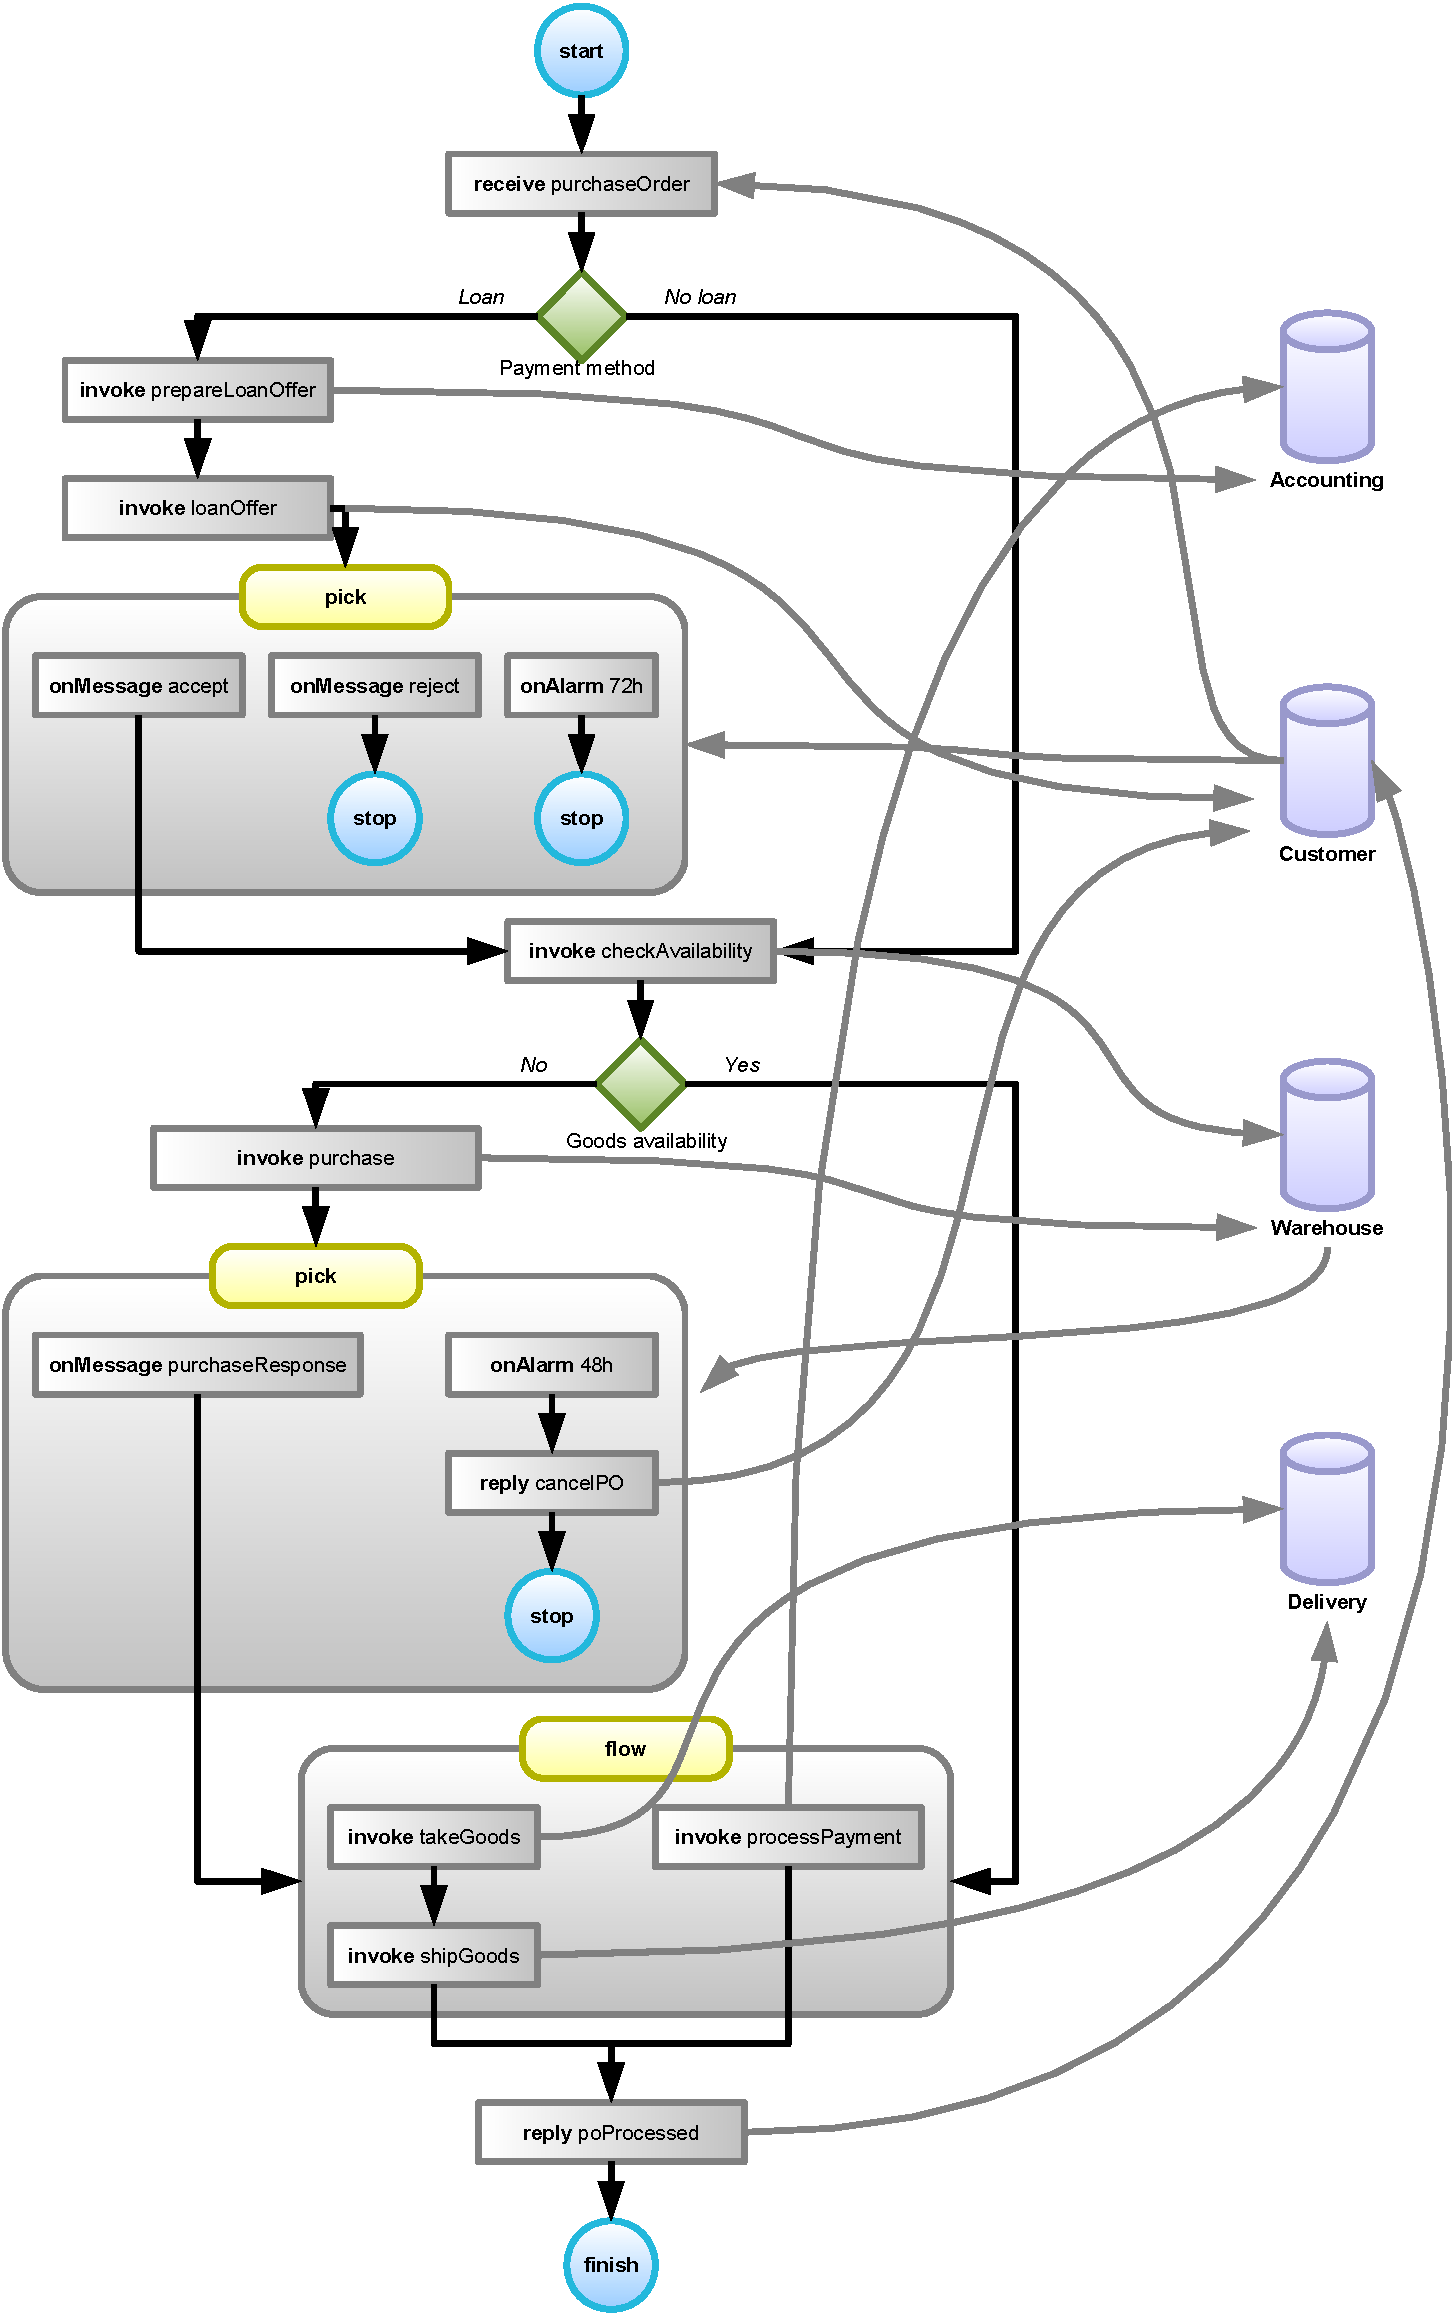
\includegraphics[height=\textheight]{content/sample-usecase/bpel-process}
    \caption{Simplified view of a BPEL process that handles purchase orders.}
    \label{fig:bpel-process}
\end{figure}

Consider the BPEL process depicted on Figure~\ref{fig:bpel-process}. It orchestrates four web services to process a purchase order. For the sake of clarity, we have removed the \emph{assign} BPEL instructions from the process diagram, normally required to prepare and reuse the messages exchanged with the involved web services. The first part of the process handles the payment options. If the customer asks for a loan, then the process will make an offer using the \emph{accounting} web service. The customer can then accept or reject it. The asynchronous \emph{pick} BPEL construction defines an alarm that will be fired after 72 hours to discard the process instance if the customer does not reply in time to the loan offer. The second part checks for the ordered goods availability with the warehouse web service. If some goods are not available, they will be ordered. In order to match quality of service requirements, the purchase is  canceled if the warehouse does not manage to purchase the missing goods within 48 hours. The third an last part of the process handles the payment and prepares the goods delivery. Finally, the customer is notified that the purchase has successfully completed.

% ........................................................................... %

\section{Business protocols extraction}

% ........................................................................... %

\begin{figure}[tbhp]
    \centering
    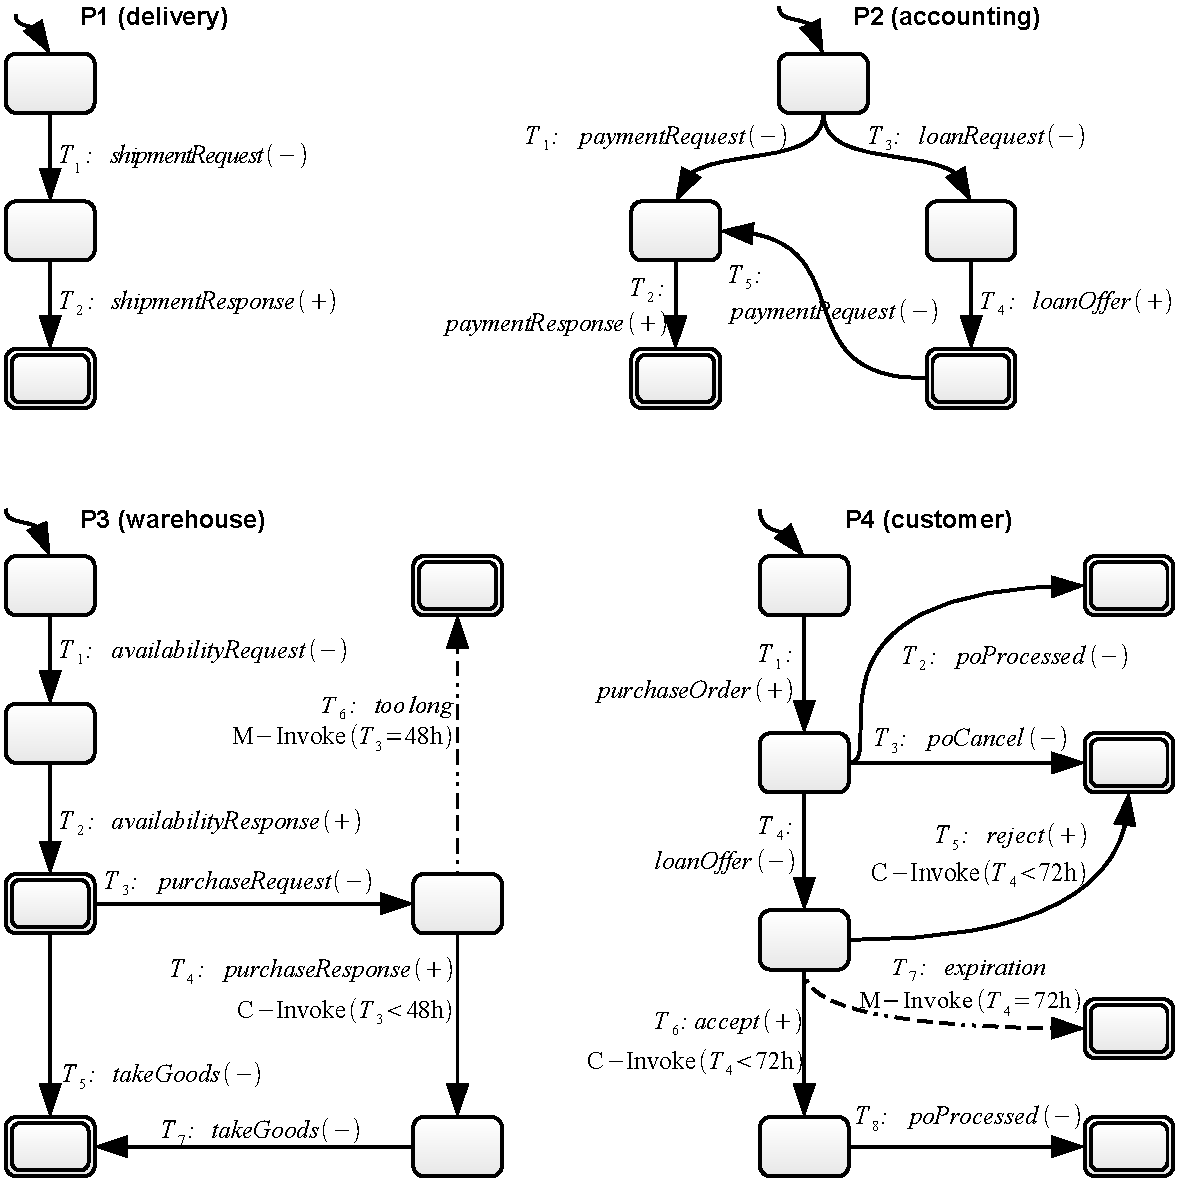
\includegraphics[width=\textwidth]{content/sample-usecase/bpel-protocols}
    \caption{Timed protocols extracted from the BPEL process of Figure~\ref{fig:bpel-process}.}
    \label{fig:bpel-protocols}
\end{figure}

Based on this BPEL process definition, we extract the timed protocols that the process supports when interacting with its partner services.
To do this, we use our multi-party protocol BPEL extractor, and we then obtain the protocol governing the interaction of the process with each of the partner services by filtering the multi-party protocol based on each service partner link.
The resulting protocols are shown in Figure~\ref{fig:bpel-protocols}.
Figure~\ref{fig:bpel-complete-warehouse} shows instead the protocol of the warehouse service we are planning to use as one of the services invoked by our process.

\begin{figure}[tbhp]
    \centering
    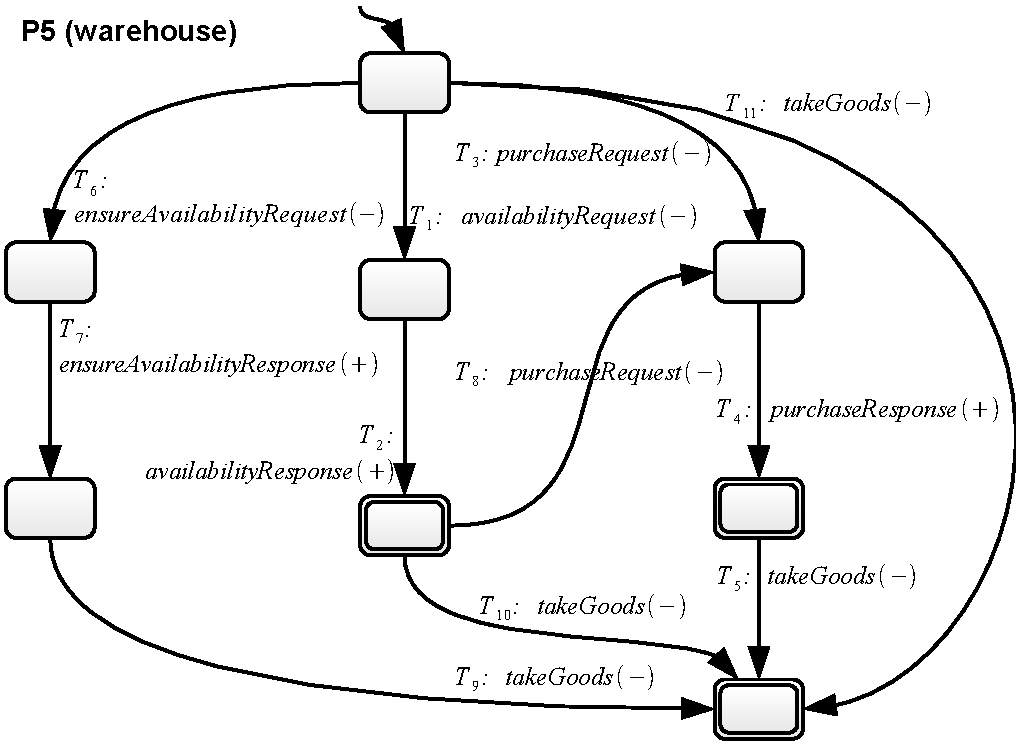
\includegraphics[width=\textwidth]{content/sample-usecase/bpel-warehouse-protocol}
    \caption{The complete warehouse service protocol.}
    \label{fig:bpel-complete-warehouse}
\end{figure}

% ........................................................................... %

\section{Protocol analysis}

% ........................................................................... %

\begin{figure}[tbhp]
    \centering
    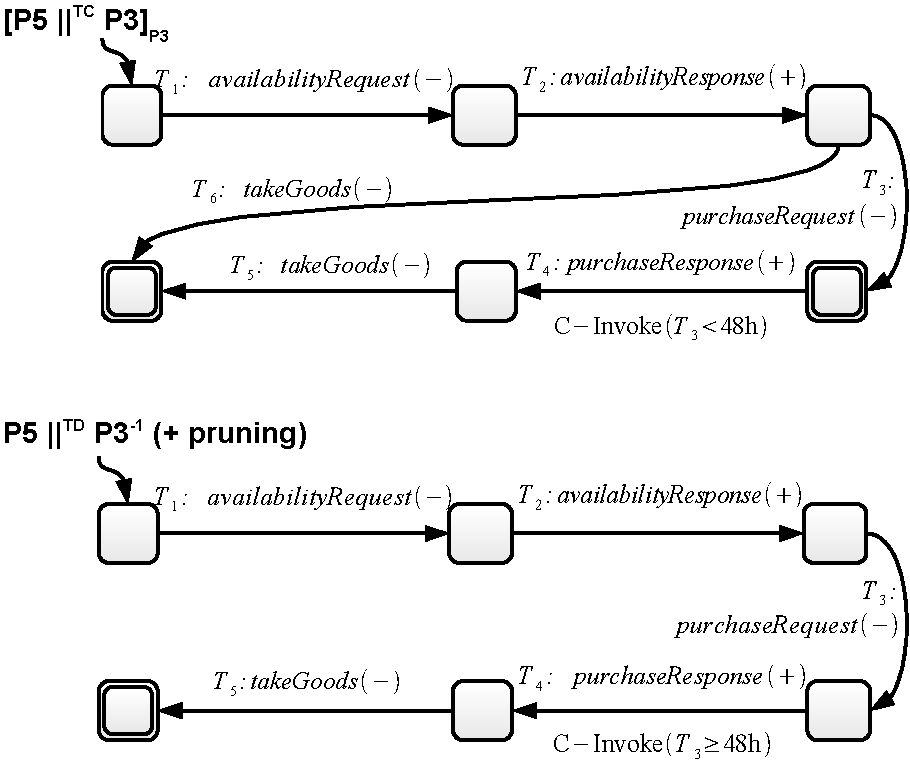
\includegraphics[width=\textwidth]{content/sample-usecase/bpel-warehouse-protocol-diff}
    \caption{Analysis of the common and differing conversations supported by $P_3$ and $P_5$.}
    \label{fig:bpel-warehouse-diff}
\end{figure}

We next apply the protocol analysis operators to assess compatibility between the protocols supported by our process and the protocols of the services we plan to use. For this, we assume that either the protocol or BPEL definition (from which we extract the protocol) of these services is available.
Figure~\ref{fig:bpel-warehouse-diff}) shows the results of this analysis for the warehouse service. In particular,
the compatible composition operator $P_5 \intersop P_3$ gives the set of the conversations that can occur between protocols $P_3$ and $P_5$.
Ideally, we would want this set to be equal to the conversations supported by $P_3$, which means that $P_5$ is fully compatible with $P_3$.\\

However, in our example, we do not have such luck. In fact we see that the conversations supported by the compatible composition are a subset of those supported by $P_3$.
The Figure further shows the conversations that are supported by the process but not by our partner service $P_5$ (which is empty in case of full compatibility), as well as the conversations that the partner supports but that the process does not support. The first of these two combined protocol is obtained by computing the inverse $P_3'$ of $P_3$ and then the difference $P_3^{-1} \diffop P_5$. The latter is instead computed as  $P_5 \diffop P_3^{-1}$. As we will examine later, all these combined protocols will become helpful in examining if and which changes need to be made to the process.\\

In particular, while the first combined protocol of  Figure~\ref{fig:bpel-warehouse-diff} (compatible composition) tells us what we can do, the second one denotes what our process is prevented from doing when using this partner (hence we call these \emph{prevented interactions}), while the third one denotes conversations that the partner would support, but we are not leveraging due to how we implemented the process. We call these \emph{neglected interactions}.\\

It is interesting to note that no compatibility problem would have been spotted in the case of business protocols without timing constraints \cite{FTBB}. Indeed, the untimed version of $P_5$ would have supported all of the conversations of the untimed version of $P_3$.

% ........................................................................... %

\section{Managing partial replaceability scenarios}

% ........................................................................... %

By looking at the three combined protocols, the developer can assess if the selected service is a good fit or not, and how to handle situations of partial replaceability or of no replaceability.
In general, this depends on the specific business purpose of the process. For example, the service I am planning to invoke may not support a $cancelPO$  operation, but I may be willing to take the risk and use it anyways even if cancellations are not allowed, for example because it offers cheaper rates.
Or, conversely, the selected service supports several forms of payments (accessed via different protocols) but my process can only support one of them, and we may be fine with it as for example our company only issues payments via credit card and not via bank transfers.\\

Alternatively, we can modify the process definition to adapt it to the service we are using, either to:
\begin{enumerate}
  
  \item ensure that our process does not generate conversations our partner cannot understand, or
  
  \item leverage conversations supported by our selected services (e.g., extend our process to support bank transfers).
  
\end{enumerate}

As another example, in our process, we can remove the \emph{onAlarm 48h} handler of the second \emph{pick} complex activity, so that the process will wait for the $purchaseResponse$ message to arrive, thereby removing the problematic temporal constraints in the extracted expected warehouse protocol. However, the process may find itself being put on hold indefinitely if a problem occurs on the warehouse service and it does not send a $purchaseResponse$ message back.\\

Another solution is to generate a protocol adapter \cite{BenatallahCGNT05} to reconcile the differences.
It can be done with the ServiceMosaic tools using an aspect-oriented framework \cite{KongdenfhaSBC06} where adapters are plugged through \emph{advices} written in BPEL. The adapter is be developed as follows. The \emph{pointcut} is triggered when a $purchaseRequest$ message is received. The advice is a BPEL process where an alarm starts counting from the reception of the $purchaseRequest$ message. If the service does not send a $purchaseResponse$ withing the next 48 hours, then the adapter drops it when the warehouse service sends it afterwards. The BPEL engine will have already woken up the process instance by then, and taken action by replying to the client partner link with a $cancelPO$ message.\\

Finally, it should be noted that for most BPEL engines, a message is simply dropped when it cannot be dispatched to any process instance for which it is waiting. An exception is then usually raised and logged inside the BPEL engine. In this example the adapter would be useful for diminishing the number of internally-thrown exceptions (raising exceptions has a significant performance cost). The choice of developing this adapter should be balanced in light of its development cost compared to the (limited) benefits, as BPEL engines can provide a form of ``implicit'' adapter in very specific mismatches cases such as this one.

% ........................................................................... %


\chapter{Conclusion and perspectives}
\label{chap:conclusion}
% ........................................................................... %

We conclude this document by summarizing the contributions. We then provide research and application perspectives beyond this work. Finally, we recall the publications on which this work is based.

% ........................................................................... %

\section{Summary}

% ........................................................................... %

This work has revisited, formalized and further extended the concepts presented in \cite{FTBB,BBFC04,BCT-CAISE03,KBBB+04} by providing an extended model for web services business protocols that supports timing abstractions. The level of abstraction that drove the design of this model was developed on the grounds of a study of real-world scenarios related to web services. The model can be leveraged for fine-grained protocol compatibility and replaceability analysis based on a set of protocol manipulation and comparison operators. We showed that the decision problems surrounding their implementation are decidable, thanks to the mapping and the identification of a novel class of timed automata which is closed under complementation and for which the language inclusion problem is decidable, all of this despite the major issue of having $\varepsilon$-labeled switches with clocks resets. Another issue was with the mapping from timed protocols to timed automata itself, as \MInvoke constraints are not easy to represent and enforce in timed automata. We also presented our initial prototype as part of the ServiceMosaic project and gave an application case study.\\

We believe that modeling and analysis techniques with formal foundations such as the ones that we have presented will help at transforming the development and the maintenance of web services based applications from an ``art'', requiring a substantial amount of manual interventions, to a model-driven process that is automated to a large extent.

% ........................................................................... %

\section{Perspectives beyond protocol analysis}

% ........................................................................... %

The concepts and techniques presented in this thesis focused on both a model for describing service protocols that includes timing constraints, and on compatibility / replaceability analysis between two such protocol instances. While already being innovative by themselves, we believe that those contributions can play a significant role when leveraged in the following contexts.

\paragraph{Protocol discovery and querying.}
It would be interesting to have protocol repositories as part of service-oriented infrastructures. Such repositories would contain timed protocols for each referenced service. They could either be based on existing repository infrastructures (e.g., UDDI and ebXML), or be standalone (e.g., given a service, point to its WSDL and timed protocol). Users and applications could then leverage them by performing queries based on protocols. Given a protocol, a repository could be queried for services whose protocols would be compatible (or replaceable).

There are several challenges linked to this type of application. The first one is to provide a large-scale, efficient physical representation for timed protocols (e.g., XML files, relational databases or XML databases). The second one is to provide an efficient indexing technique for retrieval based on compatibility and replaceability. While the timed protocol operators allow to assess either compatibility or replaceabilty between two protocols, it is clearly not advisable to take the input protocol from a query and test each protocol from the repository.

Some exploratory work has begun in the APIS Research Group, Clermont-Ferrand. The first results show promising outcomes in terms of compatibility and replaceability based services retrieval.

\paragraph{Web services testing.}
Providing automated testing at different levels (e.g., unit-testing or functional testing) is critical in today applications. This is becoming even more true in the case of service-oriented computing, as often one has no control on the services it uses. A service may respect a given protocol today, and an upgrade performed tomorrow may introduce a small change that breaks some of its clients. Worse, the changes can happen without any notification having been sent, as a service may not know all of its requesters. Both the model of timed protocols and compatibility/replaceability analysis have a significant role to play for improving web services testing practices. Indeed, protocol-based analysis can be used to detect incompatible protocol updates, while the model by itself can be used for generating conversations in the test cases.

Providing the basic infrastructure for running tests is not a big concern as extending existing tools is relatively easy (e.g., JUnit and TestNG are common testing frameworks\footnote{See \url{http://junit.org/} and \url{http://testng.org/}.}). The bigger challenges reside in generating test cases for a given service. Ideally, the set of generated test cases would provide full test coverage in a minimal number of cases. There are two research problems here:
\begin{enumerate}
  
  \item generating conversations that would each form the skeleton of a test case, and
  
  \item inject both meaningful and erroneous data in messages.
  
\end{enumerate}
In terms of conversations generation, one promising technique would be to start from timed protocols and reuse work on automated tests generation in timed automata \cite{NielsenS03,NielsenS01}.

\paragraph{Runtime stateful support.}
There is today little support in existing tools and frameworks for stateful web services. In many cases, support for stateful interactions has to be implemented manually. This means that developers need to cater with correlation and state management instead of ``just'' creating their service interfaces.

We propose to leverage the timed protocols model to facilitate the creation of stateful web services. The core idea is to keep service interfaces development simple by taking out such cross-cutting concerns out of the actual implementation code. The framework would be based on:
\begin{enumerate}
  
  \item a correlation component that intercepts messages to correlate them with service requester instances, and
  
  \item a conversation controller that checks if the intercepted message does not violate the service protocol, and
  
  \item a dispatcher that forwards messages to the actual service implementation with correlation and state information having been attached transparently to the message context.
  
\end{enumerate}

\paragraph{Timed protocol discovery and adaptation techniques.}
Existing work in ServiceMosaic projects tackled the two different problems of protocol discovery and adaptation \cite{Motahari-NezhadSBC07,BenatallahCGNT05,MBMCC-WWW07}. The protocol model being used was the untimed one from \cite{FTBB}. As such, a natural perspective is to extend it for timed protocols.

\paragraph{``Agile'' composition.}
Today, developing an application by composing existing services (e.g., in BPEL) is arguably a very static process. We envision ``agile'' frameworks based on some of the components above for facilitating the development and the maintenance of service-based compositions. In this perspective, timed protocols play a critical role (both the model and compatibility / replaceability analysis). The following frameworks would be part of this.
\begin{itemize}
  
  \item A development framework that would support the development of a composition using BPEL. It would allow developing the composition without specifying some or all of the services to be involved. Then, it would be able to query a protocols repository for compatible services, meaning that it would allow for \emph{rapid prototyping} by testing different combinations of services. Also, the framework would deal with the assembly details so that developers can almost ``drag and drop'' services in BPEL processes. Finally, it would also assist in developing adapters when services protocols would not be completely compatible with the BPEL process. Conversely, it would assist in adapting the BPEL process itself if the developer does not want to create adapters.
  
  \item A runtime framework would assist when changes get necessary. Indeed, a given service may have to be replaced, either because of unavailability or simply because the composition developers have a compelling reason to do so. In this regard, we can note that having test cases and running them periodically could be useful for rapidly spotting composition breakages. The framework would query a repository for replaceability to find a new service. Again, it would assist in developing adapters or changing the BPEL process definition so as to respect business protocols. In particular, such a framework would make it easier to cope with failures by reducing replacement costs and delays.
  
\end{itemize}

% ........................................................................... %

\section{Publications}

% ........................................................................... %

Parts and preliminary versions of this work have been published.

We started in \cite{BCPT05a,BBFC+05b} with a simple extension of business protocols that featured only \MInvoke constraints. We had introduced protocol operator algorithms tailored for the model, but it suffered from  expressiveness problems. While many \CInvoke constraints could be encoded using \MInvoke-based constructions, many complex ones could not. Also, the \MInvoke constraints always referred to the last action, which is a strong limitation by itself. Finally, the model suffered a states explosion problem when encoding \CInvoke constraints using \MInvoke primitives. The timed protocol model presented here subsumes this initial work.

The model evolved up to a new model presented in \cite{PongeBCT07} which features complex \CInvoke and \MInvoke constraints. It also introduces the reuse of the framework of timed automata for deriving the timed protocol operator properties. The model presented in this thesis contains a few tweaks that make it more expressive with respect to the \MInvoke constraints.

The approach has been presented as part of the larger ServiceMosaic project in \cite{BCTPM06-SM}. A demonstration featuring the ServiceMosaic tools was given in \cite{NezhadSBCPT07}.

\subsubsection{International refereed conferences}
\begin{itemize}

	\item Julien Ponge, Farouk Toumani, Boualem Benatallah and Fabio Casati. \textbf{Fine-grained Compatibility and Replaceability Analysis of Timed Web Service Protocols}. \emph{In the 26th International Conference on Conceptual Modeling (ER).} Auckland, New Zealand. November 2007.
	
	\item Boualem Benatallah, Fabio Casati, Julien Ponge and Farouk Toumani. \textbf{On Temporal Abstractions of Web Services Protocols}. \emph{Proceedings of CAiSE Forum 2005.} Porto, Portugal. June 2005.

\end{itemize}

\subsubsection{National refereed conferences}
\begin{itemize}

	\item Boualem Benatallah, Fabio Casati, Julien Ponge, Farouk Toumani. \textbf{Compatibility and replaceability analysis for timed web service protocols}. \emph{In BDA 2005}. Saint-Malo, France. October 2005.

\end{itemize}

\subsubsection{Refereed journals}
\begin{itemize}
    
    \item Julien Ponge, Boualem Benatallah, Fabio Casati and Farouk Toumani. \textbf{Analysis and Applications of Timed Service Protocols}. To appear in ACM Transactions on Software Engineering and Methodology (TOSEM).

	\item Boualem Benatallah, Fabio Casati, Farouk Toumani, Julien Ponge and Hamid Reza Motahari Nezhad. \textbf{Service Mosaic: A Model-Driven Framework for Web Services Life-Cycle Management}. \emph{IEEE Internet Computing, vol. 10, no. 4, pp. 55-63}. July/August 2006.

\end{itemize}

\subsubsection{Refereed workshops and demonstrations}
\begin{itemize}

	\item Hamid Motahari, Regis Saint-Paul, Boualem Benatallah, Fabio Casati, Julien Ponge and Farouk Toumani. \textbf{ServiceMosaic: Interactive Analysis and Manipulations of Service Conversations}. \emph{In International Conference on Data Engineering (ICDE'07).} Istanbul, Turkey. April 2007.
	
	\item Julien Ponge, \textbf{A New Model For Web Services Timed Business Protocols}. \emph{Atelier ``Conception des systemes d'information et services Web''- Conf\'erence INFORSID. Hammamet}. Tunisia, May 2006.
	
	\item Julien Ponge, \textbf{Modeling and Analysing Web Services Protocols}. \emph{In IBM PhD Student Symposium at ICSOC 2005}. Amsterdam, The Netherlands, December 2005.

\end{itemize}

% ........................................................................... %

% ........................................................................... %


% ........................................................................... %

\bibliographystyle{plainnat}
\bibliography{biblio}

\appendix

\part{Appendix}

% ........................................................................... %

\chapter{Proofs}
\label{chap:proofs}

% ........................................................................... %

\section{Proof of Theorem~\ref{thm:mi-expressiveness}}
\label{proof:mi-expressiveness}

% ........................................................................... %

\begin{proof}
%
We need to show that $\varepsilon$-transitions in protocol timed automata cannot always be removed, i.e., there are protocol timed automata for which there doesn't exist equivalent automata without $\varepsilon$-transitions. To do that, we exhibit the protocol timed automaton $A$ depicted on Figure~\ref{fig:precise-time} and use the notions of \emph{precise time} and \emph{precise actions} that were introduced in the Theorem~24 of \cite{BBVD+99} as a tool to identify timed languages that can only be recognized by timed automata featuring $\varepsilon$-transitions. The proof is virtually the same as the one of Corollary~29 in \cite{BBVD+99}.

It is easy to check that $A$ is a protocol timed automaton. $A$ presents 2 $\varepsilon$-transitions lying on directed cycles, hence we don't know if they can be removed using the techniques presented in Section~8 in \cite{BBVD+99}.

Let us now suppose that $\mathcal{L}(A)$ can be recognized by a timed automaton $A'$ without any $\varepsilon$-transition. Note that $A'$ is free of diagonal constraints (e.g., constraints of the form $x - y \;\#\; c$). $A'$ can be rendered disjunction-free without any loss of generality (see \cite{BBVD+99} for techniques and discussion). In order to leverage the Theorem~24 of \cite{BBVD+99}, we define $C_{\mbox{max}} = 1$ (no constant in the guards of $A$ is larger than $1$). Let also $\delta > 0$. $A$ can recognize timed words of the form
$$
  (b, \delta_1) \cdot (b, \delta_2) \cdots (b, \delta_{d - 1}) \cdot (a, d) \cdot (a, d + 1) \cdots
$$
where $d \in \N$, $d \geq C_{\mbox{max}}$ and $\delta_i \in (i-1, i) \setminus \delta \N$ for all $0 < i < d$. Let $P$ a path of $A'$ that accepts such a timed word. Given that the $a$-labeled events occur at integer times, their occurrences should be \emph{precise} in $P$. Also, $d \geq C_{\mbox{max}}$, hence from Theorem~24 of \cite{BBVD+99}, there exist some occurrence of $b$ that should be precise in $P$ which is not possible as $\delta_i \not\in \delta \N$ for any $0 < i < d$. Consequently,  $\mathcal{L}(A)$ cannot be recognized by a timed automaton without $\varepsilon$-transitions.
%
\end{proof}

% ........................................................................... %

\section{Proof of Lemma~\ref{lemma:inhib}}

% ........................................................................... %

\begin{proof}
$\inhib(g) =
    (x_1 - x \;\mathtt{not}(\#_1)\; k_1 - k) \vee 
    \cdots \vee 
    (x_j - x \;\mathtt{not}(\#_j)\; k_j - k) \vee
    (x_{j+1} - x_{j+1}' \;\mathtt{not}(\#_{j+1})\; k_{j+1}) \vee
    \cdots \vee 
    (x_{m} - x_{m}' \;\mathtt{not}(\#_{m})\; k_{m})$

For every $i \in \{1, \cdots, j \}$, note that $(x_i - x \;\mathtt{not}(\#_i)\; k_i - k)$ continuously evaluates to either $\mathtt{true}$ or $\mathtt{false}$ while the current location is $l$. Also, note that when $(x = k)$ is satisfied,
$$(x_i - x \;\mathtt{not}(\#_i)\; k_i - k) = (x_i \;\mathtt{not}(\#_i)\; k_i)$$
which is the exact negation of the clause $(x_i \;\#_i\; k_i) \in g'$.

For every $i \in \{j+1, \cdots, m\}$, $(x_{i} - x_{i}' \;\mathtt{not}(\#_{i})\; k_{i})$ is the negation of the clause $(x_{i} - x_{i}' \;\#_{i}\; k_{i}) \in g'$.

Consequently, when any clause of $g'$ is $\mathtt{false}$, $\inhib(g) = \mathtt{true}$ and, conversely, when every clause of $g'$ is $\mathtt{true}$ then $\inhib(g) = \mathtt{false}$.
\label{proof:inhib}
\end{proof}

% ........................................................................... %

\section{Proof of Lemma~\ref{lemma:permits}}

% ........................................................................... %

\begin{proof}
Let us check the implication.
$$
(g_j = \mathtt{false}) \bigvee (\permits(g_j) = \mathtt{false}) \wedge (\permits(g_i) = \mathtt{true}) = \mathtt{true}
$$
is equivalent to
$$
(\permits(g_j) = \mathtt{true}) \bigvee (\permits(g_j) = \mathtt{false}) \wedge (\permits(g_i) = \mathtt{true}) = \mathtt{true}
$$
which reduces to
$$
\underbrace{(\permits(g_j) = \mathtt{true})}_{\mathtt{false} \mbox{ \tiny{as} } g_j = \mathtt{true}} \bigvee \underbrace{(\permits(g_i) = \mathtt{true}) = \mathtt{true}}_{\permits(g_i) = \mathtt{true}}
$$
and the implication is verified. Indeed, $\permits(g_i) = \mathtt{true}$, else this would mean that the switch whose guard is $\widetilde{g_i}$ had already been activated.
\label{proof:permits}
\end{proof}

% ........................................................................... %

\section{Proof of Theorem~\ref{thm:mi-enforcement}}

% ........................................................................... %

\begin{proof}
Let us compute the cases where $\inhib(g)$ evaluates to $\mathtt{false}$. We assume that $y \in Y$ is the clock that is reset on every switch whose target location is $l$. We compute and expand the negation:
\begin{align*}
    \neg\permits(g) & = (x > k) \\
    & \wedge ((x \leq k) \vee (x - y \leq k)) \\
    & \wedge ((x \leq k) \vee (x - y > k) \vee \neg\inhib(g)) \\
    & \wedge ((x \neq k) \vee \neg\inhib(g)) \\  
   \intertext{we make a first development:}
    & = ((x = k) \vee (x \geq k) \wedge (x - y \leq k)) \\
    & \wedge ((x < k) \vee (x \neq k) \wedge (x - y > k) \\
    & \vee (x \neq k) \wedge \neg\inhib(g) \\
    & \vee (x \leq k) \wedge \neg\inhib(g) \\
    & \vee (x - y > k) \wedge \neg\inhib(g) \\
    & \vee \neg\inhib(g)) \\
    \intertext{and a second one:}
    & = (x = k) \wedge \neg\inhib(g) \\
    & \vee (x = k) \wedge (x - y > k) \wedge \neg\inhib(g) && \text{\texttt{false}} \\
    & \vee (x > k) \wedge (x - y \leq k) \wedge \neg\inhib(g) \\
    & \vee (x = k) \wedge (x - y \leq k) \wedge \neg\inhib(g) \\
    & \vee (x \geq k) \wedge (x - y \leq k) \wedge \neg\inhib(g) \\
    \intertext{by reducing the last 3 disjunctions:}
    \neg\permits(g) & = (x = k) \wedge \neg\inhib(g) \\
    & \vee (x \geq k) \wedge (x - y \leq k) \wedge \neg\inhib(g) \\
    & = (x \geq k) \wedge (x - y \leq k) \wedge \neg\inhib(g) && \text{(1)}
\end{align*}
(1): $((x = k) = \mathtt{true}) \Longrightarrow ((x - y \leq k) = \mathtt{true})$.

This means that $\permits(g)$ disables switches when:
\begin{enumerate}
  
  \item $(x = k)$ is satisfied as well as $g'$, resulting in the $\varepsilon$-labeled switch whose guard is $g$ to be enabled, or
  
  \item $l$ was entered before $(x = k)$ was satisfied, $g'$ was satisfied when $(x = k)$ was, and the current clocks valuation satisfies $(x \geq k)$, forcing the $\varepsilon$-labeled switch to be taken.
  
\end{enumerate}
\label{proof:mi-enforcement}
\end{proof}

% ........................................................................... %

\section{Proof of Lemma \ref{lemma:pta-determinism}}
\label{proof:pta-determinism}

% ........................................................................... %

\begin{proof}
Let us consider a location $l$ that offers several switches, including $n > 0$ $\varepsilon$-labeled ones. By considering two switches from $l$, three cases are possible.
\begin{enumerate}

	\item The switches have both labels that are not $\varepsilon$. By definition their guards are disjoint.
	
	\item One switch $e_i$ ($i \in \{1, \cdots, n\}$) has $\varepsilon$ as its label with a guard
	$$(g_i \bigwedge\limits_{1 \leq j \neq i \leq n} \permits(g_j))$$
	and the other switch has a label that is not $\varepsilon$ and a guard
	$$(g \bigwedge\limits_{1 \leq j \leq n} \permits(g_j))$$
	The product of the guards contains a sub-clause $(g_i \wedge \permits(g_i))$ which is false: the guards are disjoint.
	
	\item The two switches have $\varepsilon$ as their label. The product of their guards will make a sub-clause of the following form to appear:
	$$(x_i = k_i) \wedge g_i' \wedge \permits(g_j) \wedge (x_j = k_j) \wedge g_j' \wedge \permits(g_i)$$
	($i$ and $j$ belong to $\{1, \cdots, n\}$ with $i \neq j$). As $\permits(g_j) \wedge g_j'$ is false, the guards are disjoint.

\end{enumerate}
\end{proof}

% ........................................................................... %

\section{Proof of Theorem~\ref{thm:closure-intersection}}

% ........................................................................... %

\begin{proof}
The proposed constructions yields a timed automaton that qualifies as a protocol timed automaton with respect to Definition~\ref{def:pta}. Let us have a look at the specificities of protocol timed automata that required an extension of the construction compared to regular timed automata \cite{RADLD94}.

The introduction of $\varepsilon$-labeled switches in the resulting automaton preserves determinism. Indeed, given a pair of those switches, the step 3 of the construction makes sure that either both switches are triggered at the same time, or one will be triggered before the other one. Without the addition of a third $\varepsilon$-labeled switch that corresponds to both being triggered at the same time, and without the addition of inequality clauses in the original switches, there could be indeterminism, thus effectively breaking closure under intersection.

Finally, the guards rewriting step keeps them sound with respect to their original clocks. Indeed, consider any clock $x_e$ from either of the input automata and its mapped clocks set $\{ x_{e,e1}, x_{e,e2}, \cdots, x_{e,en} \}$ ($n > 0$) in the resulting automaton. Then per construction:
\begin{itemize}
  
  \item $x_e$ is reset implies that for any $i \in \{1, 2, \cdots, n\}$, $x_{e,ei}$ is also reset, and
  
  \item $i \in \{1, 2, \cdots, n\}$, $x_{e,ei}$ is reset implies that $x_e$ is also reset.
  
\end{itemize}
Consequently, the guard of both the input and resulting automata exhibit the same behaviors since the clocks that they refer to have synchronous resets.
\label{proof:closure-intersection}
\end{proof}

% ........................................................................... %

\section{Proof of Theorem~\ref{thm:closure-complement}}

% ........................................................................... %

\begin{proof}
The construction of $A^*$ adds one location $q$ to $A$ as well as one new switch per symbol of the alphabet and per location of $A$ plus $q$. We first show that the construction preserves determinism, and that given an input symbol, it can be recognized for any clocks valuation when the current location doesn't have any $\varepsilon$-labeled switch.

As every new switch guard is defined as the negation of the disjunctions of the guards of the switches from the same label, the intersection of the guards of every switch on the same label for a location $l$ is necessarily false, meaning that those guards are disjoint. In the case where a location $l$ does not offer any $\varepsilon$-labeled switch, it is also easy to check that the disjunction of the guards of the switches having the same label from $l$ is true as in \cite{RADLD94}.

Let us now consider a location $l$ having $n > 0$ $\varepsilon$-labeled switches $g_{\varepsilon i}$ ($1 \leq i \leq n$). We also consider any symbol $a$ of the alphabet and the $m > 0$ guards of the $a$-labeled switches from $l$: $\{g_1, \cdots, g_m \}$ (again, given $1 \leq j \leq m$, $g_j$ is considered without its $\permits$ function clauses). Let us compute the disjunction of the $a$-labeled switches guards:
$$
  \left( g_1 \bigwedge\limits_{1 \leq i \leq n} \permits(g_{\varepsilon i}) \right)
  \bigvee \cdots \bigvee
  \left( g_m \bigwedge\limits_{1 \leq i \leq n} \permits(g_{\varepsilon m}) \right)
$$
By construction there exists $j \in \{1, \cdots, m\}$ such that $g_j = \neg \left( \bigvee\limits_{1 \leq k \neq j \leq m} g_k \right)$, hence the previous disjunction reduces to:
$$ \bigwedge\limits_{1 \leq i \leq n} \permits(g_{\varepsilon i}) $$
which means that $a$ is recognized from $l$ under \MInvoke semantics. However, $\overline{A}$ must also recognize $a$ when this expression evaluates to false, which is clearly not possible from $l$. 

Let $v$ be a clocks valuation such that $a$ is to be recognized and
$$ v \models \left( \bigwedge\limits_{1 \leq i \leq n} \permits(g_{\varepsilon i}) = \mathtt{false} \right)$$
We can make the following remarks:
\begin{enumerate}
  
  \item the current location is not $l$ anymore as a $\varepsilon$-labeled switch has been taken for the first clock valuation that stopped satisfying the previous expression, and
  
  \item the current location change through the $\varepsilon$-labeled switch was instantaneous.
  
\end{enumerate}
Let us call the current location $l'$. By construction, it offers $a$-labeled switches. From the remarks above, the guard of every switch satisfies 
$$ \neg \left( \bigwedge\limits_{1 \leq i \leq n} \permits(g_{\varepsilon i}) \right)$$
for the clocks valuation $v$.

Consequently, $a$ can always be recognized from $l$ and the locations available through its $\varepsilon$-labeled switches:
$$
  \left( \bigwedge\limits_{1 \leq i \leq n} \permits(g_{\varepsilon i}) \right)
  \bigvee
  \neg \left( \bigwedge\limits_{1 \leq i \leq n} \permits(g_{\varepsilon i}) \right)
  = \mathtt{true}
$$
\label{proof:closure-complement}
\end{proof}

% ........................................................................... %
% ........................................................................... %

\chapter{Semantics of protocol timed automata}
\label{chap:pta-semantics}

% ........................................................................... %

The semantics of protocol timed automata over an infinite labeled transition system $\mathcal{S}_A$ are borrowed from those of event-clock automata \cite{RALF94}, another class of timed automata defined over $\T = \Rpos \cup \{ \perp \}$.

\begin{definition}[Protocol timed automata semantics]
The semantic of a protocol timed automaton $A = (L, L^0, L^f, X \cup Y, E, \Sigma)$ is given by the (infinite) LTS $\mathcal{S}_A = (S, s_0, \rightarrow, \Sigma)$ where:
\begin{itemize}

    \item $S = L \times \T^X$ is the set of states $(l, v)$ (also called \emph{configurations}) comprising each a location and a clocks valuation,

    \item $s_0 = (l_0, v_0)$ with $l_0 \in L^0$ and $v_0(x) = \perp$ $\forall x \in X$,

    \item $\rightarrow$ is the transition relation:
    \begin{itemize}

        \item action transitions: $(l, v) \stackrel{a}{\longrightarrow} (l', v')$ if and only if there exists
        $e = (l, g, a, r, l') \in E$ such that $v \models g$, $v' = [r \leftarrow 0]v$ 

        \item time transitions: $\stackrel{d}{\longrightarrow} (l, v')$ for $d \in \Rpos$ if $\forall x \in X$:
        \begin{itemize}
          \item if $v(x) \neq \perp$ then $v'(x) = v(x) + d$, else
          \item if $v(x) = \perp$ then $v'(x) = \perp$.
        \end{itemize}

    \end{itemize}

\end{itemize}
\end{definition}

A timed word $w$ is recognized by a protocol timed automaton $A$ if there exists a run over $\mathcal{S}_A$: $(l_0, v_0) \stackrel{d_0}{\longrightarrow} (l_0, v_1) \stackrel{a}{\longrightarrow} (l_1, v_1) \stackrel{\cdots}{\longrightarrow} \cdots \stackrel{\cdots}{\longrightarrow} (l_n, v_n)$ such that $l_n \in L^F$.\\

Reachability analysis is the key to most of the analysis techniques on timed automata. The formal grounds for this reside in the ability to group ``similar'' configurations that each comprise the current location and a clocks valuation. Those groups, called regions, are built using an equivalence relation between the configurations that represent the states of the (infinite) labeled transition system associated to a timed automaton \cite{RADLD94}. We adapt an equivalence relation for protocol timed automata.\\

We define an equivalence relation between the states of $\mathcal{S}_A$, denoted as $\cong$. We denote the integer part of a real-valued number $r \in \Rpos$ as $\lfloor r \rfloor$ and its fractional part as $\{ r \}$ (e.g., $\lfloor 2.55 \rfloor = 2$ and $\{ 2.55 \} = 0.55$).

\begin{definition}
Two configurations $(l, v)$ and $(l', v')$ are \emph{equivalent}, denoted as $(l, v) \cong (l', v')$ if $l = l'$ and:
\begin{enumerate}
  
  \item $\forall x \in X$:
  \begin{itemize}
    \item if $v(x) = \perp$ then $v'(x) = \perp$, else
    \item $\lfloor v(x) \rfloor = \lfloor v'(x) \rfloor$ or both $v(x) > c_x$ and $v'(x) > c_x$
  \end{itemize}
  
   \item $\forall x,y \in X$ such as $v(x) \leq c_x$ and $v(y) \leq c_y$, then $\{v(x)\} \leq \{v(y)\}$ if and only if $\{v'(x)\} \leq \{v'(y)\}$

  \item $\forall x \in X$ such as $v(x) \leq c_x$, $\{v(x)\} = 0$ if and only if $\{v(x)\} = 0$.
  
\end{enumerate}
\end{definition}

% ........................................................................... %

\chapter{An overview of UPPAAL}
\label{chap:uppaal}

% ........................................................................... %

We present here the model used in UPPAAL which is based on timed automata. Then, we present the query language of UPPAAL before finishing with the tools that it provides.

% ........................................................................... %

\section{UPPAAL model and query language}

% ........................................................................... %

UPPAAL uses an hybrid extension of timed automata as a model and a subset of TCTL as a query language to express properties. Briefly, an hybrid system \cite{alur97symbolic} features both continuous (e.g., variables in $\R$) and discrete behavior (e.g., variables in $\N$). This allows mixing discrete variables such as booleans or integers with clocks in the models that are processed by UPPAAL. Those discrete variables can be used in guards, invariants and be reset on switches just like a clock would be. Actually, a timed automaton can be viewed as a linear hybrid automaton whose continuous variables evolve at a constant rate \cite{alur97symbolic}. Further pointers on hybrid automata can be found in \cite{Miller00, HYTECH, ACHH93}. \\

\begin{figure}[htbp]
    \centering
    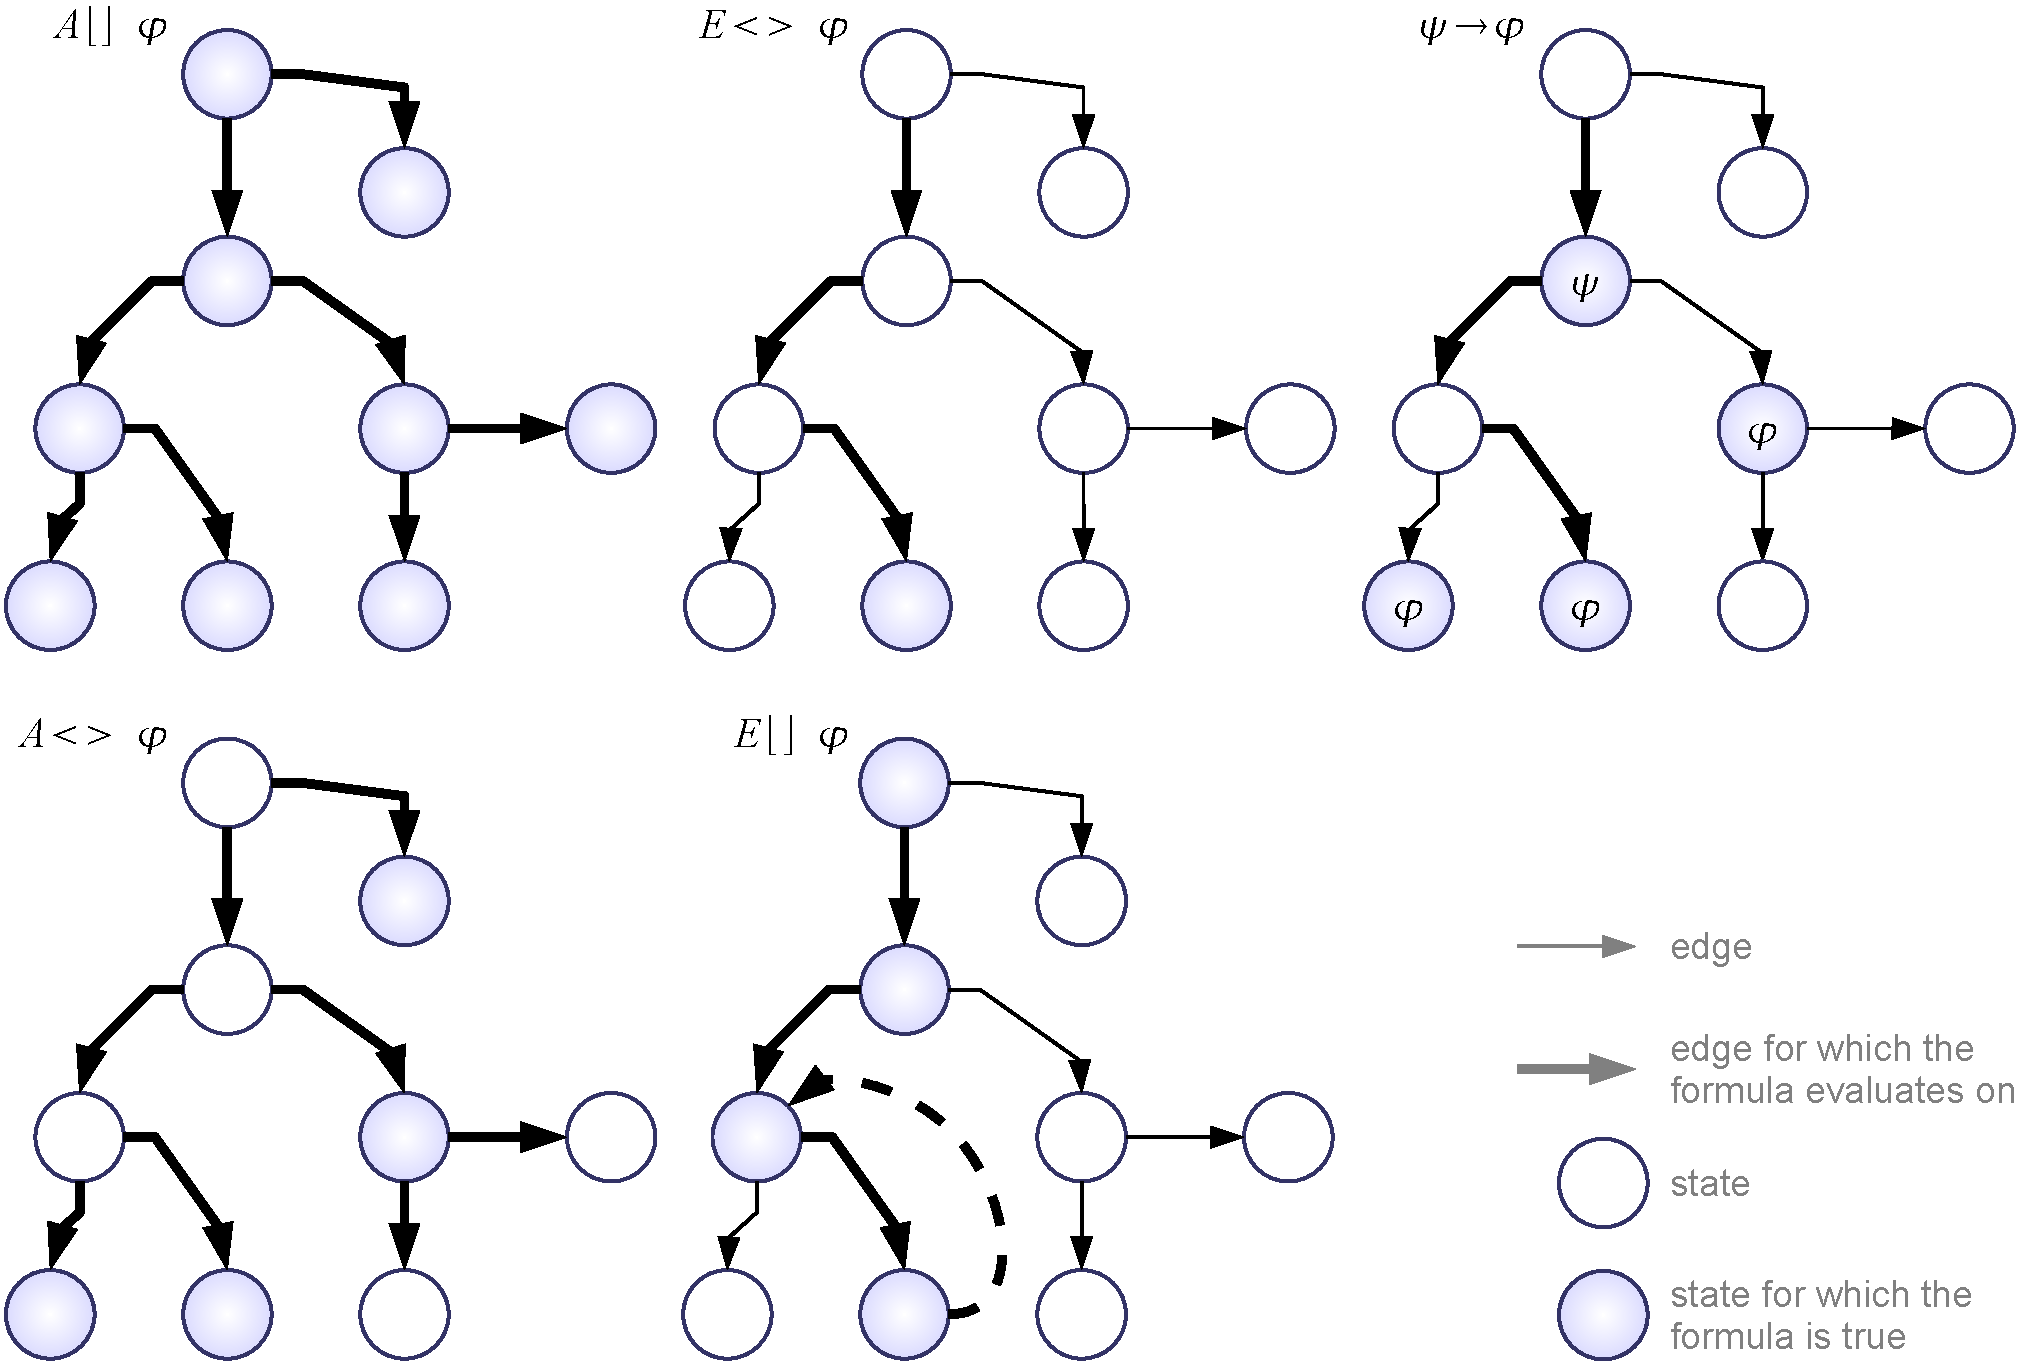
\includegraphics[width=\textwidth]{content/timed-automata/uppaal-path-formulae}
    \begin{flushright}
    	\textit{(source: \cite{UPPAAL})}
    \end{flushright}
    \caption{The path formulae that UPPAAL supports.}
    \label{fig:uppaal-path-formulae}
\end{figure}

We summarize here the types of formula that can be defined for queries in UPPAAL as detailed in \cite{UPPAAL}. We will use Figure~\ref{fig:uppaal-path-formulae} to illustrate them. To begin with, we need \emph{state formula}. Such a formula can be made from clock constraints (e.g., $(x < 3.75) \wedge (y \geq 5)$) and tests that check if a system is in a given location or not (e.g., $P.l$ is true when the system $P$ is currently in the $l$ location). By combining them using boolean conjunctions and disjunctions, it is possible to define complex state formulae such as $\varphi = (x < 3.75) \wedge (y \geq 5) \wedge P.l$. There is also a special state formula $\mathtt{deadlock}$ that is true when neither the current extended state $(l, v)$ offers an outgoing action transition nor there exists a time successor $(l, v')$ that does so. Using state formulae as a basis, the path formulae that can be expressed have been summarized in Table~\ref{tab:uppaal-path-formulae}.\\

\begin{table}[htbp]
\footnotesize
\centering
\begin{tabular}{|p{3cm}|p{7cm}|p{2cm}|}
  
  \hline
  
  \textit{Formula} &
  \textit{Semantic} &
  \textit{Analysis} \\
  
  \hline
  
  $E\Diamond \varphi$ &
  There exists a path to a state $(l, v)$ that verifies $\varphi$. &
  Reachability \\
  
  \hline
  
  $A\Box \varphi$ &
  Every reachable state $(l, v)$ satisfies $\varphi$. &
  Safety \\
  
  \hline
  
  $E\Box \varphi$ &
  There exists a path to a state $(l, v)$ with no outgoing transition that satisfies $\varphi$, or there exists an infinite path where $\varphi$ is satisfied by all states at some point. &
  Safety \\
  
  \hline
  
  $A\Diamond \varphi$ &
  For every possible path, there exists a state $(l, v)$ such that $\varphi$ is satisfied. &
  Liveness \\
  
  \hline
  
  $\varphi \rightarrow \psi$, or equivalently $A\Box (\varphi \Rightarrow A\Diamond \psi)$ &
  Given a state $(l_1, v_1)$ satisfying $\varphi$, every path starting from it contains a state $(l_2, v_2)$ such that $\psi$ is satisfied. &
  Liveness \\
  
  \hline
  
\end{tabular}
\caption{Semantics of the path formulae supported by UPPAAL (a subset of TCTL).}
\label{tab:uppaal-path-formulae}
\end{table}

Going back to the examples of verifications that we expressed as \emph{property 1} and \emph{property 2} on Figure~\ref{fig:light-verification-inclusion}, the properties can be checked by UPPAAL using the following formulae:
\begin{itemize}
  
  \item \emph{property 1}: $E\Diamond (\mathsf{Model.off \wedge x = 10})$ (the location $\mathsf{Model.off}$ is reachable while the clock $x$ has a valuation of 10)
  
  \item \emph{property 2}: $E\Diamond (\mathsf{Model.off \wedge x = 1})$ (there is a path to a state in the LTS of $\mathsf{Model}$ such that the current location is $\mathsf{Model.off}$ and the current valuation of the clock $x$ is 1).
  
\end{itemize}
UPPAAL evaluates the first property to \texttt{true} and the second one to \texttt{false}. Please note that ``undesirable'' properties (i.e., the ones that should normally evaluate to \texttt{false}) are expressed \emph{positively} in UPPAAL (as opposed to \emph{negatively} using a boolean negation operator).\\

UPPAAL supports a subset of TCTL. which provides more path formulae. Also, TCTL allows nested path formulae, something that UPPAAL does not support.

% ........................................................................... %

\section{UPPAAL tools}

% ........................................................................... %

\begin{figure}[htbp]
    \centering
    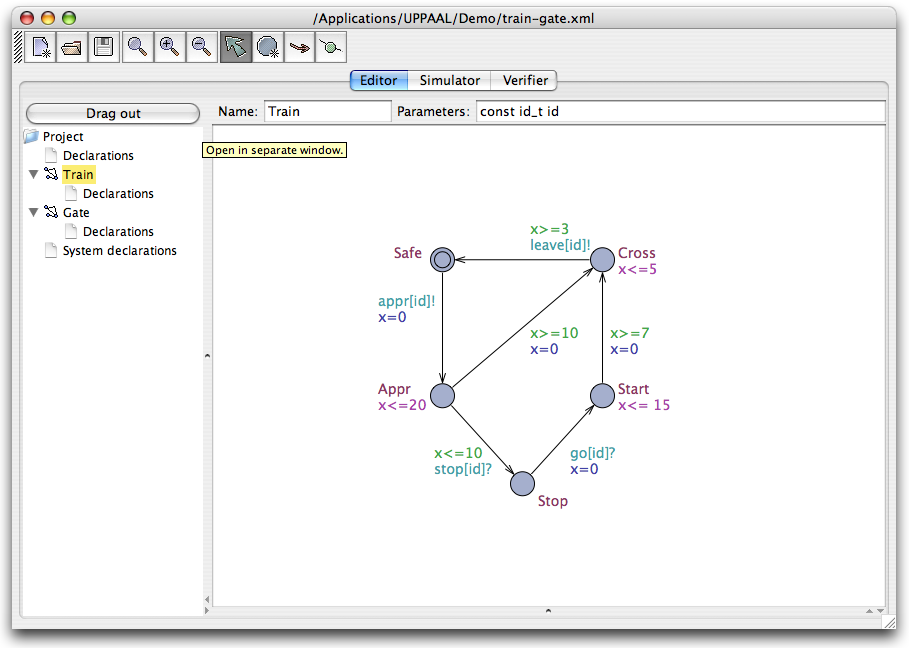
\includegraphics[width=\textwidth]{content/timed-automata/uppaal-1}
    \caption{UPPAAL: modeling environment.}
    \label{fig:uppaal-1}
\end{figure}

UPPAAL comprises two main components:
\begin{enumerate}
  
  \item a command-line model checker called \emph{verifyta}, written in C and ported to Unix variants (Linux, *BSD), Windows and Mac OS X, and
  
  \item a graphical user interface (GUI) written in Java.
  
\end{enumerate}
The UPPAAL GUI (see Figure~\ref{fig:uppaal-1}) is a comprehensive environment for modeling, simulating and verifying systems represented as timed automata. The editor allows to define a set of (usually interacting) systems (e.g., the gate, barrier controller and train systems of the examples found in \cite{RADLD94} or the light controller of Figure~\ref{fig:light-verification-inclusion}).\\

\begin{figure}[htbp]
    \centering
    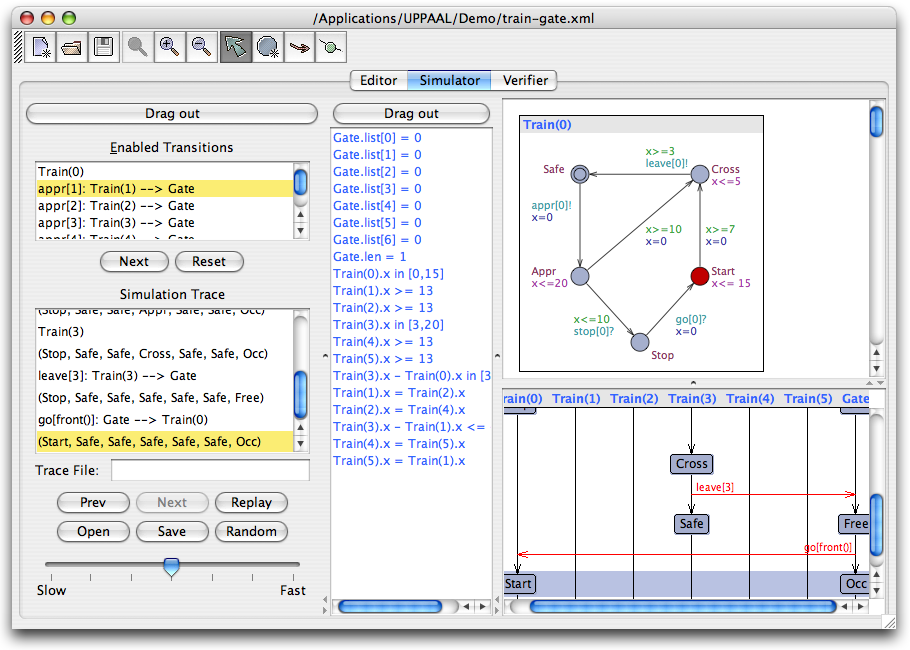
\includegraphics[width=\textwidth]{content/timed-automata/uppaal-2}
    \caption{UPPAAL: simulation environment.}
    \label{fig:uppaal-2}
\end{figure}

The simulator component (see Figure~\ref{fig:uppaal-2}) allows users to simulate the execution of the systems to see which switches are taken, what are the clocks valuation ranges at each step and so on. The simulation can be run automatically by the tool: when several switches can be enabled from a given location, the next switch is selected randomly. Otherwise, the user can select which switch should be taken next at each step. In the later case, the simulator acts as a kind of step-by-step debugger as found for traditional programming using languages such as C/C++ or Java.\\

\begin{figure}[htbp]
    \centering
    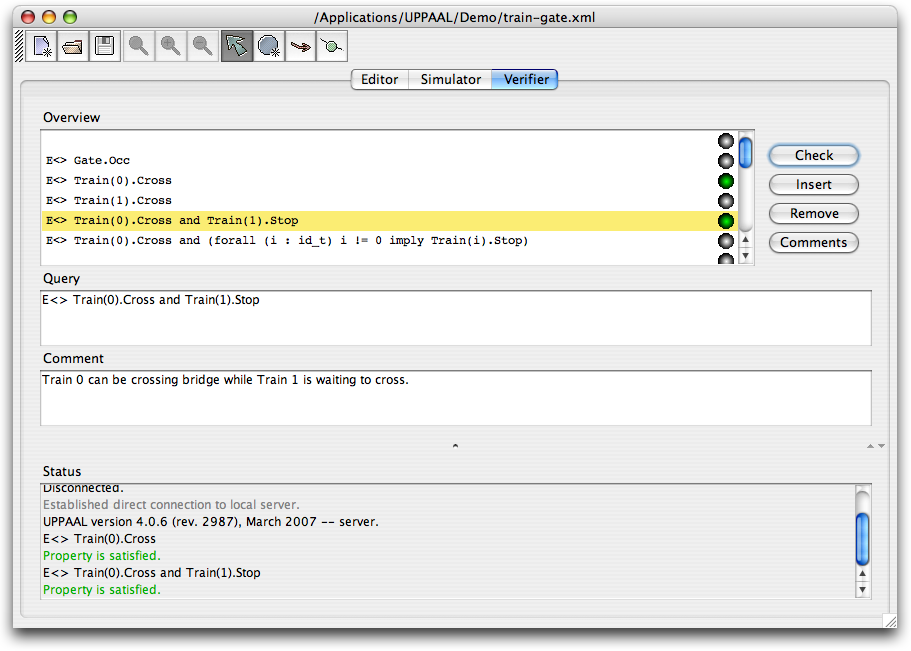
\includegraphics[width=\textwidth]{content/timed-automata/uppaal-3}
    \caption{UPPAAL: verification environment.}
    \label{fig:uppaal-3}
\end{figure}

Finally, the verification component (see Figure~\ref{fig:uppaal-3}) allows to perform model checking tasks by encoding requests in (timed) temporal logics. In fact, this component is directly using the command-line \emph{verifyta} tool to perform the verifications.

% ........................................................................... %

\chapter{UPPAAL and protocol timed automata}
\label{chap:uppaal-pta}

% ........................................................................... %

As we will see hereafter, checking emptiness on protocol timed automata with UPPAAL is not straightforward. We first explain the issues in converting a protocol timed automaton into an automaton that UPPAAL can process. We then propose a procedure for performing a semantic-preserving conversion. Finally, we illustrate it on the protocol $P_2'$ of Figure~\ref{fig:uppaal-pta}.\\

% ........................................................................... %

\section{Conversion issues}

% ........................................................................... %

We use UPPAAL for verifying whether a timed protocol is empty or not, i.e., whether it supports at least a conversation or not. To do that, we consider each final location of a protocol timed automaton and leverage UPPAAL to verify if it can be reached from its initial location or not (i.e., there exists a timed word whose execution over the protocol timed automaton ends in the considered final location). The language that is recognized by a protocol timed automaton is not empty as long as one final location can be reached.\\

This checking is however not straightforward. Indeed, a protocol timed automaton cannot be directly given to UPPAAL:
\begin{enumerate}
  
  \item clocks in UPPAAL are defined over $\Rpos$ whereas protocol timed automata are defined over $\Rpos \cup \{ \perp \}$, and
  
  \item in protocol timed automata, the clocks are initially set to $\perp$ and keep this value until they have been reset for the first time while in classical timed automata (and hence for UPPAAL) they start from 0 and immediately start their progression, and
  
  \item UPPAAL expects the guards to be conjunctions of atomic clock constraints (e.g., $x \:\#\; k$) and diagonal constraints (e.g., $x - y \;\#\; k$).
  
\end{enumerate}

% ........................................................................... %

\section{Conversion technique}

% ........................................................................... %

These differences can be overcome as UPPAAL does not work on \emph{strict} timed automata, but rather uses an hybrid model where non-clock variables can be defined, reset on switches and used in guards \cite{UPPAAL}. We propose the following procedure for checking protocol timed automata emptiness using UPPAAL. It has been implemented as part of the ServiceMosaic Protocols project presented earlier.

\begin{procedure}
Let us consider a protocol timed automaton $A$. The first step is to generate a UPPAAL model \texttt{Process} as follows.
\begin{enumerate}

	\item Remove the disjunctions in the guards of $A$:
	\begin{enumerate}
		\item obtain the abstract syntax tree (AST) of each constraint, then
		\item use an AST visitor \cite{Gamma95}: for each disjunction node, split into two switches (the disjunction node is replaced by the left-hand node in one switch guard, and by the right-hand node in the other switch guard)
		\item repeat until no AST contains a disjunction.
	\end{enumerate}
	
	\item Assign a unique boolean variable $b_x$ (initially set to \texttt{false}) to each switch that is set to \texttt{true} in the switch reset. This encodes $\perp$.
	
	\item Using an AST visitor, for each constraint clause $(x \;\#\; k)$ where $k \neq \perp$, rewrite as $(x \;\#\; k) \wedge (b_x = \mathtt{true})$ (note that it does not make sense to write a diagonal constraint comparing to $\perp$). When $k = \perp$, rewrite it as $(x \;\#\; k) \wedge (b_x = \mathtt{false})$.

\end{enumerate}

Finally, to check for emptiness: for each final location $l$, the corresponding TCTL property to be passed to UPPAAL is \texttt{E<> Process.l} and the procedure stops at the first final location $l$ such that the property is met, else the the timed language is empty.
\label{proc:emptiness}
\end{procedure}

We can point out the following remarks.
\begin{itemize}
  \item A procedure can be derived from this one to verify event-recording timed automata using UPPAAL.
  \item The procedure generates an automaton which is not a protocol timed automaton.
  \item Removing disjunctions from guards had already been discussed in \cite{BBVD+99} -- in fact the technique is the same.
\end{itemize}

% ........................................................................... %

\section{Sample conversion and emptiness checking}

% ........................................................................... %

\begin{figure}[htbp]
  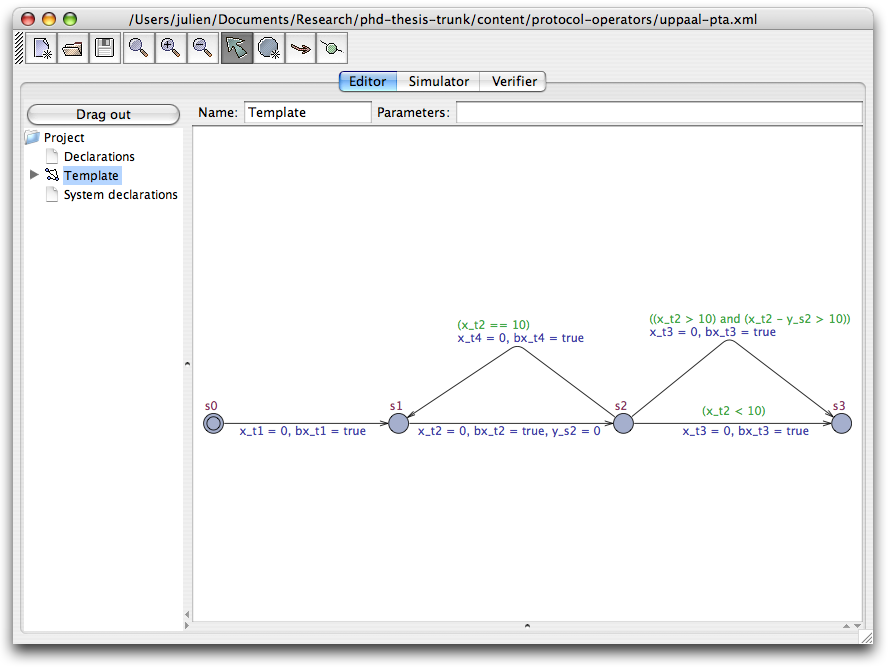
\includegraphics[width=\textwidth]{content/protocol-operators/uppaal-pta-1}
  \vspace{-0.5cm}
  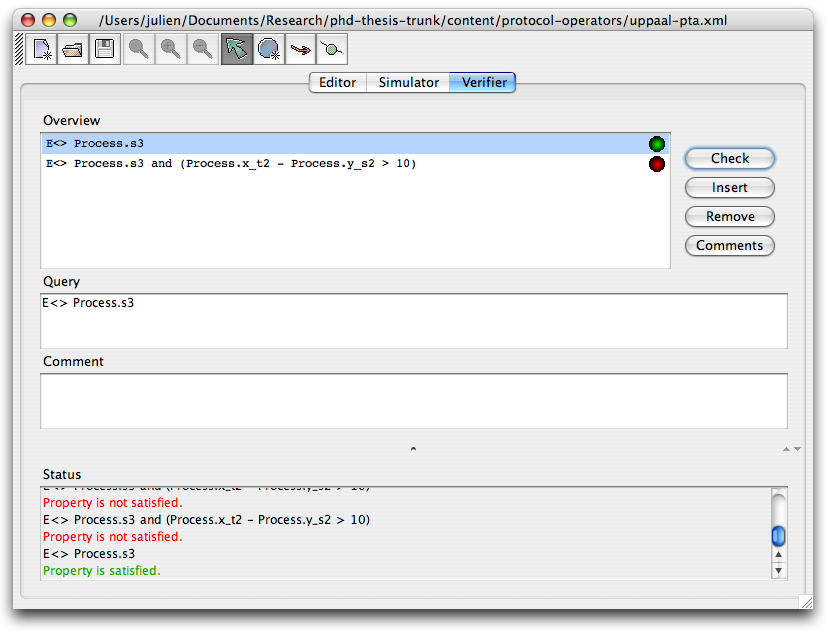
\includegraphics[width=\textwidth]{content/protocol-operators/uppaal-pta-2}
  \caption{Emptiness checking of protocol timed automata with UPPAAL.}
  \label{fig:uppaal-pta}
\end{figure}

Let us consider the protocol timed automaton $P_2$ of Figure~\ref{fig:sample-intersection}. The conversion to a UPPAAL automaton is illustrated on Figure~\ref{fig:uppaal-pta} along with the emptiness checking. As we can see, the conversion involves adding an extra switch between $S_2'$ and $S_3'$ as the permits clause is disjunctive and UPPAAL forbids disjunctions in guards.\\

The emptiness checking is performed using the following query:
$$ E\Diamond\; \mathtt{Process.s3} $$
On the figure, we have also added another query:
$$ E\Diamond\; \mathtt{Process.s3} \;\mathtt{and}\; (\mathtt{Process.x\_t2} - \mathtt{Process.y\_s2} > 10)$$
that checks that the $\varepsilon$-labeled switch is enforced. Indeed, due to the configuration of this automaton, the added switch with a guard \texttt{((x\_t2 > 10) and (x\_t2 - y\_s2 > 10))} cannot be taken under \MInvoke semantics.\\

Here is the corresponding UPPAAL automaton XML file:
{
  \footnotesize
  \verbatiminput{content/protocol-operators/uppaal-pta.xml}
}

Here is also the UPPAAL queries file:
{
  \footnotesize
  \verbatiminput{content/protocol-operators/uppaal-pta.q}
}

% ........................................................................... %

\backmatter

\cleardoublepage
% ........................................................................... %

\thispagestyle{plain}

~\vfill

\begin{footnotesize}

\noindent
\textbf{Notice regarding the production of this document}\\

\noindent
This document was produced with a \LaTeX-based tools chain and the \textsf{memoir} class by Peter Wilson which is available from CTAN at \url{http://www.ctan.org/tex-archive/macros/latex/contrib/memoir/}.\\

\noindent
Screen captures of various softwares appear in several places of this document. Those images were captured by the author for the sole purpose of illustration.\\

\noindent
The figures were produced using the \textsf{OpenOffice.org Draw} software which is available from \url{http://www.openoffice.org/}. Some graphic elements used in the figures originate from the \textsf{Crystal Project} and the \textsf{Tango Desktop Project}. They are used in due respect to their (permissive) licenses agreements. Refer to \url{http://everaldo.com/crystal/} and \url{http://tango.freedesktop.org/Tango_Desktop_Project} for more informations.

\end{footnotesize}

\vfill

% ........................................................................... %

% ........................................................................... %

\end{document}

% ........................................................................... %

